\documentclass[letterpaper,12pt]{report}
\usepackage[utf8]{inputenc} \usepackage[top=2.cm, bottom=2cm, left=2cm, right=2cm]{geometry} 
\usepackage{mathrsfs} 
\usepackage{palatino} 
\usepackage[font=it]{caption}
\usepackage{graphicx,amsmath,amssymb,rotating,booktabs,url,color,enumitem}	\DeclareUrlCommand\url{\def\UrlLeft{<}\def\UrlRight{>}\urlstyle{tt}}  
\usepackage{upgreek}

\usepackage[style=/home/filip/d/biblatex-phys/phys, articletitle=true, biblabel=enumerate, chaptertitle=true, pageranges=true, 
			sorting=none, isbn=false, url=false, doi=false, eprint=false, hyperref=true, firstinits   = true]{biblatex}
\addbibresource{fdphd.bib}

\newcommand{\E}{\mathbf{E}}
\newcommand{\D}{\mathbf{\tilde{D}}}
\newcommand{\Dsd}{\mathbf{D}}
\newcommand{\B}{\mathbf{B}}
\newcommand{\HH}{\mathbf{\tilde{H}}}
\newcommand{\HHsd}{\mathbf{H}}
\newcommand{\epsrl}{\varepsilon_r}
\newcommand{\murl}{\mu_r}
%\newcommand{\epsrl}{\varepsilon^{\rm(Loc)}_r}
%\newcommand{\murl}{\mu^{\rm(Loc)}_r}
\newcommand{\Neff}{N_{\text{eff} }}
\newcommand{\Zeff}{Z_{\text{eff} }}
\newcommand{\eeff}{\varepsilon_{\text{eff} }}
\newcommand{\meff}{\mu_{\text{eff} }}
\newcommand{\ii}{{\mathrm i}}
\newcommand{\rr}{{\mathbf{r}}}
\newcommand{\brho}{\boldsymbol{\rho}}
\newcommand{\kk}{{\mathbf{k}}}
\newcommand{\KK}{{\mathbf{K}}}
\newcommand{\epsr}{{\varepsilon_r}}

\newcommand{\add}[1]{\color{blue}#1\color{black}{}}
\newcommand{\rmv}[1]{\color{grey}\ensuremath{\vdash}#1\ensuremath{\dashv}\color{black}{}}
\newcommand{\mdf}[1]{{\color{red}#1}}
\newcommand{\coloruse}{\marginpar{\scriptsize
\add%
{added}\\ \mdf%
{modified}\\ \rmv%
{deleted} }}



\begin{document}
\begin{center}
	\Large{\textbf{
Czech Technical University in Prague\\
Faculty of Nuclear Sciences and Physical Engineering\\ 
%Department of Physical Electronics\\
}}
 \vspace{3cm}


\includegraphics[width=5cm]{img/LogoCVUT}
\vspace{2cm}

\huge{\textbf{\scshape Dissertation thesis}}\\
\vspace{5mm}
{\LARGE\textbf{Metamaterials for the terahertz spectral range\\}}
\end{center}

\date{ } 			


 \vfill
\begin{minipage}{.99\textwidth}
\Large{\textbf{Prague 2016}} \hfill \Large{\textbf{Filip Dominec}}
\end{minipage}


\thispagestyle{empty} \newpage \setcounter{page}{1}

% --------------------------------------------------------------------------------
\chapter*{Bibliografický záznam}
 %\begin{tabular}{rl}
 %Author: 	&\textbf{Filip Dominec}\\
 %Advisor: 	&\textbf{Mgr. Filip Kadlec, Dr.}\\
 %Consultant: 	&\textbf{Doc. Ing. Ivan Richter, Dr.}\\ 
 %Year:		&\textbf{2015}\\
 %\end{tabular}

\bgroup \def\arraystretch{1.5}
\noindent\begin{tabular}{p{.25\linewidth}p{.7\linewidth}}
	Autor:				&\textbf{Ing. Filip Dominec} \\ 
					~	&České vysoké učení technické v Praze\\ 
					~	&Fakulta jaderná a fyzikálně inženýrská\\  
					~	&Katedra fyzikální elektroniky\\
Název práce:			&\textbf{Metamateriály pro terahertzovou spektrální oblast} \\
Studijní program:		&\textbf{Aplikace přírodních věd} \\
Studijní obor:			&\textbf{Fyzikální inženýrství} \\
Školitel:				&\textbf{Mgr. Filip Kadlec, Dr.} \\
					~	&Fyzikální ústav\\ 
					~	&Akademie věd České republiky\\  %Na Slovance 2,  182 21 Praha 8, Czech Republic 
Školitel specialista:	&\textbf{Doc. Ing. Ivan Richter, Dr.} \\
					~	&České vysoké učení technické v Praze\\ 
					~	&Fakulta jaderná a fyzikálně inženýrská\\  
					~	&Katedra fyzikální elektroniky\\
Akademický rok:			&\textbf{2015/16} \\			%% TODO is this the correct format?
Počet stran:			&\textbf{\pageref{enddocument}} \\  %% TODO shall give the overall page number or just that of the authored text?
Klíčová slova			&\textbf{metamateriály, fotonické krystaly, terahertzová technologie, elektrodynamické simulace, homogenizace efektivních prostředí} \\
\end{tabular}
\egroup

\thispagestyle{empty} \newpage

% --------------------------------------------------------------------------------
\chapter*{Bibliographic entry}
\bgroup \def\arraystretch{1.5}
\noindent\begin{tabular}{p{.25\linewidth}p{.7\linewidth}}
Author:					&\textbf{Ing. Filip Dominec} \\
					~	&Czech Technical University in Prague\\
					~	&Faculty of Nuclear Sciences and Physical Engineering\\ 
					~	&Department of Physical Electronics\\
Title of Dissertation:	&\textbf{Metamaterials for the terahertz spectral range} \\
Degree Programme:		&\textbf{Application of natural sciences} \\
Field of Study:			&\textbf{Physical engineering} \\
Supervisor:				&\textbf{Mgr. Filip Kadlec, Dr.} \\
					~	&Institute of Physics\\ 
					~	&Academy of Sciences of the Czech Republic\\  %Na Slovance 2,  182 21 Praha 8, Czech Republic 
Supervisor specialist:	&\textbf{Doc. Ing. Ivan Richter, Dr.} \\
					~	&Czech Technical University in Prague\\ 
					~	&Faculty of Nuclear Sciences and Physical Engineering\\  
					~	&Department of Physical Electronics\\
Academic Year:			&\textbf{2015/16} \\
Number of Pages:		&\textbf{\pageref{enddocument}} \\
Keywords				&\textbf{metamaterials, photonic crystals, terahertz technology, computational electrodynamics, homogenization of effective media} \\
\end{tabular}
\egroup
\thispagestyle{empty} \newpage

% --------------------------------------------------------------------------------
%\vspace{30mm}
%\textbf{\huge{Abstrakt} }
%\vspace{-5mm}

%\begingroup \renewcommand{\newpage}{}
\vspace{-20mm}
\chapter*{Abstrakt}
\noindent ~
% TODO přeložit
Při interakci elektromagnetických vln s periodickými strukturami lze pozorovat neobvyklé jevy, jako je záporný index lomu, fotonický zakázaný pás nebo silná prostorová disperze. Tyto struktury mohou být navrženy tak, aby se chovaly žádoucím způsobem, a označují se buďto jako metamateriály nebo jako fotonické krystaly. Část z jejich navrhovaných využití je v technice terahertzových vln, kde můžou překlenout po\-měr\-ně slabé možnosti klasických součástek.  

Teoretický základ práce vychází z elektrodynamiky prostředí s klasickou frekvenční disperzí, která je dále zobecněna na prostředí s prostorovou disperzí a na Blochovu-Floquetovu teorii vln v periodických strukturách. Závěr teoretické části se pokouší vyjasnit pojmy používané v literatuře a ukázat, že myšlenky metamateriálů i fotonických krystalů jsou ve skutečnosti starší, než se často uvádí.

Obecná teorie je doplněna příklady terahertzového chování různorodých periodických struktur, které bylo vypočteno metodou konečných diferencí v časové doméně (FDTD). V některých případech byly její výsledky podloženy jinými simulačními algoritmy nebo měřeními pomocí terahertzové spektroskopie v časové doméně.

Srovnání  různých struktur si klade za cíl srozumitelnou formou prezentovat a vy\-svět\-lit nej\-pod\-stat\-něj\-ší principy. Podobné srov\-nání zřejmě v dosavadní literatuře chy\-bě\-lo. Klíčové vý\-sledky spočí\-vají v popisu přechodu mezi režimy metamateriálu a fotonického krystalu v periodickém poli dielektrických tyčinek a v důkazech toho, že k popisu chování řady uvedených struktur je zcela nezbytné uvažovat prostorovou dispersi. V neposlední řadě práce dokládá možnosti simulačních skriptů, které autor vyvinul a uveřejnil na internetu s úmyslem podpořit další výzkum v této oblasti. 

\vspace{0mm}
%\chapter*{Abstract} 
{\let\clearpage\relax\chapter*{Abstract}}
\noindent
Unusual phenomena such as negative index of refraction, photonic band gaps, or strong spatial dispersion are observed when electromagnetic waves interact with periodic structures. These can be designed to manipulate the wave in an advantageous way, and are known either as metamaterials or photonic crystals. Part of their proposed applications are for the terahertz technology, where they may address relatively poor performance of classical components.

The theoretical background is derived from the electrodynamics of media with classical dispersion, which is later generalized to spatially dispersive media and to the Bloch-Floquet theory of waves in periodic structures. The end of the theoretical part attempts to clarify the terminology used in the literature, and to show that the concepts of metamaterials and photonic crystals are in fact older than is sometimes assumed.

The general theory is complemented with examples of the behaviour of diverse periodic structures in the terahertz range, which was numerically simulated by the finite-difference time-domain method. In some cases, the results of this simulation method were supported by other simulation algorithms or by the experimental measurement by the terahertz time-domain spectroscopy. 

The comparison of different structures encompassed in this thesis attempts to present and explain most relevant principles in a didactic way. Arguably, such a comparison was missing in the previous literature.
The key results are in the description of the transition between metamaterial and photonic crystal regimes in a periodic array of dielectric rods, and in the demonstration of the fact that considering spatial dispersion is essential for the description of the behaviour of many periodic structures.
Last but not least, the thesis demonstrates the capabilities of the simulation environment which the author developed and completely published online to stimulate further research in this field. 

% TODO Z abstraktu musí být zřejmé, co je cílem předložené práce a jakých vědeckých výsledků doktorand osobně dosáhl.
%% + attention was focused to the parts of different topics, where the author's work could contribute with new knowledge
%\endgroup

\thispagestyle{empty} \newpage
% --------------------------------------------------------------------------------
\chapter*{Acknowledgements}
Preparation of this thesis was not without difficulties. However, it appears that overcoming such difficulties is essential to gain some sort of valuable knowledge that can not be conveyed through textbooks, and of experience that can not be gained through straightforward and focused work only.  At the first place I wish to express thanks to my advisor, Dr. Filip Kadlec, and all other people who helped this project to be finished, namely Dr. Christelle Kadlec and doc. Petr Ku\v{z}el  from the Institute of Physics, and doc. Ivan Richter from the Faculty of Nuclear Engineering and Physical sciences, Czech Technical University. 

Discussions with doc. Lukáš Jelínek and prof. Jan Macháč convinced me about the value in proper handling of the theoretical background, which later proved essential for explaining the results of the thesis. During my stay in France in 2013, the collaboration with Dr. Mathias Vanwolleghem not only greatly contributed to my experience with the numerical simulations, but was also very inspiring. 

Almost surprisingly, all my scientific aspirations found a permanent and selfless support of my wife and all family members, who always had patience with my focusing on abstract problems instead of the more practical aims and with my stubborn attitude towards some of their good advices.

The numerical results presented in the thesis could be hardly obtained without the work of hundreds of volunteers contributing to the open-source scientific software: Most of the plots were made using the Matplotlib library \cite{hunter2007} and computations were based on MEEP \cite{oskooi2010meep} and MPB programs \cite{johnson2001mpb}. 

This work was financially supported by the Czech Science Foundation under Grant No. 14-25639S.

\thispagestyle{empty} \newpage

\tableofcontents
\chapter{Theory}



\add{The theoretical chapter starts with a brief review of \textit{electrodynamics of continuous media}. In its customary form without account for spatial dispersion, this topic is treated in every related textbook, so classical linear electrodynamics is introduced in a minimalistic manner.
%, avoiding many relevant topics such as  TODO, which are not essential for the description of metamaterials.  
This serves as a basis for transforming into the so-called Landau-Lifshitz formulation of electrodynamics for spatially-dispersive media, which is elaborated more in detail.}

\section{Electrodynamics of continuous media} 
\subsection{Electromagnetic wave in vacuum} % FIXME
\paragraph{Maxwell equations}  %{{{
In the realm of classical physics, the electromagnetic phenomena are governed by the \textit{Maxwell equations} in the following form.
We assume here that no free charges and no sources of currents are present: 
\begin{equation} \nabla \cdot  \D = 0, \label{eq_me1}\end{equation}  
\begin{equation} \nabla \cdot  \B = 0, \label{eq_me2}\end{equation}  
\begin{equation} \nabla \times \E = -\frac{\partial \B} {\partial t}, \label{eq_me3}\end{equation}  
\begin{equation} \nabla \times \HH =  \frac{\partial \D} {\partial t}, \label{eq_me4}\end{equation}  
where the $\E$ and $\HH$ are the electric and magnetic vector fields, and $\D$ and $\B$ are the electric and magnetic displacements,
 respectively. These two pairs of field and displacement are related in a similar way as a force is related to the deformation. %% TODO Simovski2007 regards the current J as force, and E as the deformation!
 The \textit{constitutive relations} depend on the properties of the medium the wave propagates in, and in vacuum they take the simplest possible form:
\begin{equation}		\D = \varepsilon_0	\E, \quad\quad\quad						\B = \mu_0			\HH,				 \label{eq_ce}\end{equation}
the $\varepsilon_0 = 8.85\cdot10^{-12}$ F/m being the \textit{vacuum permittivity} and $\mu_0 = 1.25\cdot10^{-6}$ H/m being the \textit{vacuum permeability}. 
Pages \pageref{starttext}--\pageref{endtext} of this thesis will be concerned with computation, interpretation, and experimental verification of the Eq. (\ref{eq_me1}--\ref{eq_me4}) solutions for specific choices of constitutive equations.
\label{starttext}
%}}}
\paragraph{Wave equation in vacuum} %{{{
The pair of first-order differential equations (\ref{eq_me3}, \ref{eq_me4}) can be converted to a single second-order differential equation. To this end, we apply an extra curl operator $\nabla\times$ from the left, and substituting from one equation into the another, we accumulate two curl operators on the left hand side and two derivatives on the right hand side: 
\begin{equation} \nabla\times (\nabla\times \E) = \nabla\times \left(- \frac{\partial \B} {\partial t}\right) = -\mu_0 \frac{\partial}{\partial t} \left(\nabla\times \HH\right) 
= -\mu_0 \frac{\partial^{2} \D}{\partial t^{2}} = -\mu_0 \varepsilon_0 \frac{\partial^{2} \E}{\partial t^{2}}.  \label{eq_elim}\end{equation}
Using the vector calculus identity
\begin{equation} \nabla\times (\nabla\times \E) \equiv \nabla (\nabla \cdot \E) - \nabla^2 \E, \label{eq_rotrot}\end{equation}
we obtain the \textit{wave equation} for the electric field in vacuum: 
\begin{equation}  \nabla (\nabla \cdot \E) - \nabla^2 \E = -\mu_0 \varepsilon_0 \frac{\partial^{2} \E}{\partial t^{2}}.  \label{eq_wave}\end{equation}
%Note this holds for each component of electric field independently. -- NOT: the divergence is not independent of other components
Starting with Eq. (\ref{eq_me4}) instead of (\ref{eq_me3}), the same result could also be easily obtained for the magnetic field $\HH$.
%}}}
\paragraph{Plane wave and sign convention} %{{{
The solutions of the linear wave equation (\ref{eq_wave}) can be decomposed as a sum of \textit{harmonic plane waves}, where \textit{harmonic} means that the amplitude depends on the time $t$ as a harmonic function (e.g. $\sin(t)$). As a \textit{plane wave} we denote such a spatial shape of the fields, that is a function of a single  scalar parameter $\kk\cdot\rr$. Assuming the wave propagates with nonzero velocity, also the spatial dependence on  $\kk\cdot\rr$ must be harmonic, and therefore 

Any other complicated shape of the fields can be decomposed into a linear superposition of more such waves and treated separately \cite{jackson1962book}. 

%Linear electrodynamics is often treated with the 
The electromagnetic field will described as a complex exponential, i.e. as a superposition of two waves differing by a mere quarter-period phase shift, one defining the real part, one the imaginary part of the field. In comparison with the intuitive description of a plane wave in terms of a cosine (or sine) function, the complex notation formally simplifies some mathematical operations, e.g. it allows to easily identify the \textit{phase of a wave as} the exponent (divided by $1/\ii$). 

%% ---- "ENGINEERING" in favor of +iwt , and then perhaps using eps = (eps' - i eps''), or getting along with all-negative eps''
%% https://www.comsol.com/support/knowledgebase/1009/    
%% http://www.tpdsci.com/tpc/RISignDv.php
%% Panofsky & Phillips 1962, p 200 ??
%% ---- "OPTICS" in favor of -iwt, then using the simpler eps = (eps' + i eps'')
 

%% TODO add figure: plane wave
Without loss of generality, we define the electric field as a function of time $t$ and position in space $\rr$, corresponding to a plane wave in the complex notation:
\begin{equation} \E(t, \rr) := \E_0\, e^{\ii\omega t - \ii\kk\cdot\rr} \label{eq_pw}\end{equation}
The plane wave is fully characterised by its \textit{amplitude vector} $\E_0$, \textit{angular frequency} $\omega$ and \textit{wave vector} $\kk$. Note that no restrictions were put to the amplitude vector $\E_0$ so far, thus Eq. (\ref{eq_pw}) can describe both \textit{transverse} wave of any polarization, with $\E_0 \perp \kk$, and \textit{longitudinal wave} with $\E_0 || \kk$.

An important note shall be made on the sign convention for the complex wave. 
We use the `engineering' convention of time dependence: $e^{+\ii \omega t}$, but this is only due to the author's feeling that it is more natural when the wave phase grows in time. 
It is used in  roughly a half of the literature 
(e.g. \cite[p. 9]{engheta2006book}
\cite[pp. 21, 99]{krowne2007book}
\cite[chap. 1-4, 6, 9, 10]{eleftheriades2005book})
.  In the remaining half,
(e.g. \cite[chap. 5, 7, 8]{eleftheriades2005book}),
\cite{jackson1962book}, 
\cite{veselago1968},
\cite{born1999book}, \cite[p. 5]{noginov2011book}), 
the opposite, `optical', convention is used with time dependence of $e^{-\ii \omega t}$. 
The choice of $e^{+\ii\omega t}$ or $e^{-\ii\omega t}$ determines the sign of imaginary part in virtually all complex quantities discussed in this thesis, but with correct interpretation it makes no difference in the physical conclusions as it is only a formal simplification.
In the real world, observable fields do not have any imaginary component so the real part of the result has to be taken. 

In the $e^{+\ii\omega t}$ convention, many parameters of a passive (lossy) system are restricted to have \textit{negative imaginary part}.  An additional complication arises from that a part of the authors using $e^{+\ii\omega t}$ convention wish to represent the imaginary part as \textit{positive}, and they define complex quantities as, e.g., $\varepsilon = \varepsilon' - \ii \varepsilon''$, % TODO verify if this is e.g. "Wallen2011-Anti-resonant response of ..."
thus in their case $\varepsilon''\equiv -\text{Im}(\varepsilon)$. Thorough the thesis, we however represent the real and imaginary parts naturally as $\varepsilon := \varepsilon' + \ii \varepsilon'' $.
%}}}
\paragraph{Dispersion relations in vacuum} %{{{
Only some combinations of ($\E_0, \omega, \kk$) provide a physical solution of the wave equation (\ref{eq_wave}). In vacuum, the allowed solutions can be obtained by first substituting the differential operators by their equivalents for a particular plane wave: %TODO explain
\begin{equation} \nabla \rightarrow -\ii\kk, \quad\quad\quad 
\frac{\partial} {\partial t} \rightarrow \ii\omega, \label{eq_difftok}\end{equation}
so the wave equation (\ref{eq_wave}) can be modified the following way:
$$					\nabla (\nabla \cdot \E) - \nabla^2 \E				  =	-\mu_0 \varepsilon_0 \frac{\partial^{2} \E}{\partial t^{2}},  $$
$$				 -\ii\kk (-\ii\kk \cdot \E)  - (-\ii\kk \cdot -\ii\kk) \E = -\mu_0 \varepsilon_0 (\ii\omega)^2 \E, $$
\begin{equation}   - \kk (\kk \cdot \E)      +          k^2 \E            = +\mu_0 \varepsilon_0 \omega^{2} \E.  \label{eq_wavek}\end{equation}
The solutions of this wave equation for a harmonic plane wave divide into two groups: % TODO add reference that there is no other oslutino
\begin{enumerate}
 \item{\textit{Transverse electromagnetic waves}, with the electric field and wave vector being perpendicular, i.e. $(\kk \cdot \E) = 0$. Therefore, the \textit{dispersion relation} for a transverse plane wave in vacuum is linear:
\begin{equation} k~= \sqrt{\mu_0 \varepsilon_0}\; \omega = \frac{\omega}{c}, \label{eq_dispeq_vac}\end{equation}
where we defined the \textit{speed of light} $c := \frac{1}{\sqrt{\mu_0 \varepsilon_0}}$.
} 
 \item{\textit{Longitudinal electromagnetic waves}, with $\kk\,|| \pm \E$, require the right side of Eq. \ref{eq_wavek} to be zero. In vacuum, there is no such a solution, except for a homogeneous static electric field ($k = 0, \omega = 0$), but they may exist in a dispersive medium.} 
 \end{enumerate}
\begin{figure} \caption{Dispersion curve of a transverse electromagnetic wave in vacuum} \centering 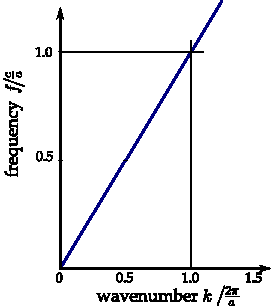
\includegraphics[width=6cm]{img/dispersion_curve_vacuum.pdf} \end{figure}
%}}}

\subsection{Local response of media to the electromagnetic field} \label{loc_response_of_media}
\paragraph{Local response definition} \label{subsection_local_resp} %{{{
In the whole chapter, we expect the medium properties to be time-invariant, linear, and homogeneous (i.e. independent of time, field amplitude and position in space, respectively). 
In this section, we focus on the special case when the medium response in point $\rr$ is not influenced by the electric field in any other point $\brho \neq \rr$. The medium is then said to be \textit{local}. 
For most media found in nature, this approximation is very close to reality and thus numerous electrodynamics textbooks tend to omit the nonlocal effects. 
However using this local theory to a wave propagating through periodic structures has a priori no justification and may lead to completely wrong results. The local theory presented here will serve as a basis for the nonlocal theory developed in following chapters.
% Applying the more familiar local electrodynamics to these structures is a mistake common to many papers. While the local theory is mathematically consistent, it predicts unusual spectral shapes and does not allow their further physical interpretation.

When an electric field $\E$ is applied, the medium responds by a change of the electric displacement $\D$ in a way that is characteristic for it. 
The immediate response of vacuum from the right side of the constitutive equations (\ref{eq_ce}) remains unchanged, but the response of the matter adds a new term called \textit{electric polarisation}. The polarisation is not instantaneous, so it is generally expressed as a convolution of the \textit{electric susceptibility} $\chi_e^{\rm(Loc)}$ with the values of electric field in the previous time $\tau$:
\begin{equation} \D(t,\rr) = \varepsilon_0 \E(t,\rr) + \varepsilon_0 \int_{-\infty}^{t}\chi_e^{\rm(Loc)}(t-\tau)\, \E(\tau,\rr)\,\mbox{d}\tau. \label{eq_loc_chi_convol}\end{equation}
Assume that a harmonic plane wave propagates through the medium, so $\E(t, \rr) := \E_0 \, e^{\ii\omega t - \ii\kk\cdot\rr}$, as given by Eq. (\ref{eq_pw}). This can be inserted in the above equation:
\begin{equation} \D(t,\rr) = \varepsilon_0 \E_0 \, e^{\ii\omega t - \ii\kk\cdot\rr} + \varepsilon_0 \int_{-\infty}^{t} \chi_e^{\rm(Loc)}(t-\tau) \, \E_0 \, e^{\ii\omega \tau - \ii\kk\cdot\rr} \,\mbox{d}\tau. \label{eq_chi_convol_harm}\end{equation}
Substituting $T:=t-\tau$, the exponent can be separated into two parts: one of which factors out of the integral, and the remaining part that turns the convolution into a temporal Fourier transform of the medium response:
$$				 \D(t,\rr) = \varepsilon_0 \E_0 \, e^{\ii\omega t - \ii\kk\cdot\rr} + \varepsilon_0 \int_{-\infty}^{0} \chi_e^{\rm(Loc)}(T) \, \E_0 \, e^{\ii\omega (t - T) - \ii\kk\cdot\rr} \,\mbox{d}T,$$
$$				 \D(t,\rr) = \varepsilon_0 \E_0 \, e^{\ii\omega t - \ii\kk\cdot\rr} + \varepsilon_0 \left( \int_{-\infty}^{0} \chi_e^{\rm(Loc)}(T)  \, e^{-\ii\omega T}\,\mbox{d}T  \right) \E_0 \, e^{\ii\omega t - \ii\kk\cdot\rr}.$$
%% NOTE that the Fourier transform is never subject to the sign change, cf. \ref{eq_kkF}
This is nothing but an application of the convolution theorem: convolution in time domain is equivalent to multiplication the in frequency domain.  %% FIXME normalisation by 2pi?
Consequently we may introduce the local \textit{relative permittivity} $\epsrl(\omega)$ as a function of frequency. It is a property of the medium that determines how strong it develops the electric displacement $\D$ in response to a harmonic wave. From Eq. (\ref{eq_ce}) it is clear that in vacuum,  $\epsrl = 1$.
\begin{equation}  \epsrl(\omega) =   \frac{\D(t,\rr)}{\varepsilon_0 \E(t,\rr)} \biggr|_{\E(t, \rr) := \E_0 \, e^{\ii\omega t - \ii\kk\cdot\rr}} = 1 + \int_{-\infty}^{0} e^{-\ii\omega T} \,\chi_e^{\rm(Loc)}(T) \,\mbox{d}T \label{eq_eps_loc}\end{equation}
%% TODO note that this is a complex-valued function, unlike chi_e(loc); and explain why it is so: that it allows to easily pack in also the information about the phase
%}}}
\paragraph{Response of a harmonic oscillator} \label{chap_lorentzmedia} %{{{
\begin{figure}[t] \caption{\textbf{a)} Illustration of how a simplified medium may respond to an electric field impulse in the shape of Dirac delta function  $E(t) = \delta(t)$. The response is composed from an instantaneous part from vacuum, $\delta(t)$, and from a delayed ringdown of one damped harmonic oscillator, described by $\chi_e^{\rm(Loc)}(t) := 2\pi \sin(2\pi t)\,e^{-x/2}$; \textbf{b)} The corresponding local permittivity $\epsrl(\omega)$, computed by Fourier transform of the response. Note that the imaginary part of permittivity is negative due to that the material is lossy (absorbs energy) and that the $e^{\ii\omega t}$ convention is used.} \label{fg_oscillator_spectrum} \centering 
	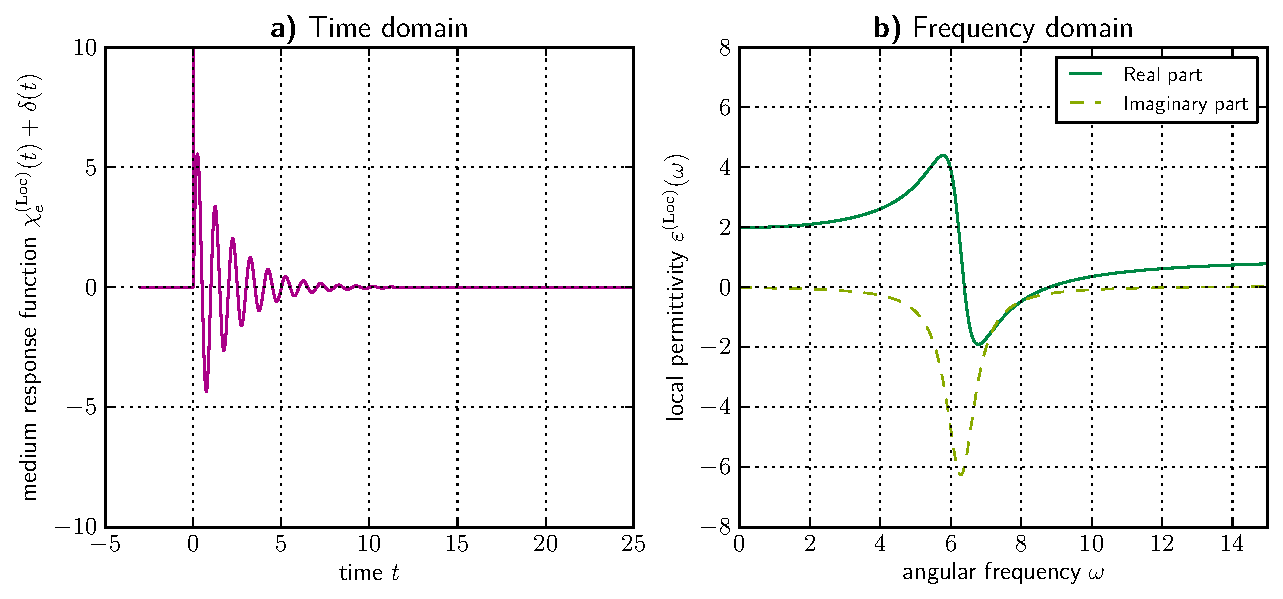
\includegraphics[width=17cm]{img/oscillator_spectrum.pdf}
\end{figure}
The response function $\chi_e(T, \mathbf{R})$ of usual media is composed of different phenomena.  Each of them may react on different time scales, and thus the medium response usually has a relatively complicated shape in the time domain.  However, to a reasonable degree of approximation, each of the contributions can be treated separately, as is demonstrated in the following.

Linear physical systems with an inertial mass, friction force and a restoring force are known as \textit{damped harmonic oscillators}.  This theory applies well to the electrons elastically bound to an atomic nucleus, as well as to the atoms elastically bound to their equilibrium position in the lattice. The molecular rotation can also be modelled as an (possibly overdamped) harmonic oscillator. Even the free electrons in conductive media can fit into the theory of harmonic oscillator provided the restoring force is set to nearly zero. The response of a harmonic oscillator is easy to describe both in time domain and frequency domain, even without the explicit use of the Fourier transform from Eq. (\ref{eq_eps_loc}). The harmonic oscillator model thus becomes a convenient starting point to approximate the response of materials.

A damped harmonic oscillator is described by a second-order differential equation:
\begin{equation} \alpha \frac{\partial^{2} x(t)}{\partial t^{2}} + \beta\frac{\partial x(t)}{\partial t} + \zeta x(t) = f(t). \label{eq_harm_osc}\end{equation}
Provided the driving term on the right hand side  is harmonic $f(t) = e^{+\ii \omega t}$, the system response is also a harmonic function, $x(t) = \chi(\omega) e^{+\ii \omega t}$. The differential equation (\ref{eq_harm_osc}) can be easily solved to show that the complex amplitude of the driven oscillations, $\chi(\omega)$, depends on the angular frequency and on the parameters $\alpha$, $\beta$ and $\zeta$ in the following way:
\begin{equation} \chi(\omega) \equiv \frac{x(t)}{f(t)} = \frac{1}{\zeta-\alpha\omega^{2} + \ii\omega\beta}  = \frac{\alpha^{-1}}{\frac{\zeta}{\alpha}-\omega^{2} + \ii\omega\frac{\beta}{\alpha}}. \label{eq_harm_osc_result}\end{equation}
The physical meaning of $\alpha$, $\beta$ and $\zeta$ is of little importance in this text, but without loss of generality the result of Eq. (\ref{eq_harm_osc_result}) can be rewritten into
\begin{equation} \chi(\omega) = \frac{F}{\omega_0^{2}-\omega^{2} + \ii\omega\gamma}, \label{eq_harm_osc_rewritten}\end{equation}
where the physical interpretation of the three (real and positive) parameters is as follows:
\begin{itemize}
 \item{$\omega_0 = \sqrt{\zeta/\alpha}$ is the angular \textit{frequency of resonance}, at which the response is pure imaginary and usually its modulus $|\chi(\omega=\omega_0)|$ is near its maximum.} 
 \item{$\gamma = \zeta/\alpha$ is the \textit{damping rate}. In time domain, it determines the time constant of exponential amplitude decay. In frequency domain, it is roughly proportional to the resonance width. } 
 \item{$F = \alpha^{-1}$ is the \textit{oscillator strength}, determining the amplitude of the response function.}
 \end{itemize}


\paragraph{Permittivity of Lorentz media} Within the approximation of relatively weak fields, the oscillators act independently of each other.
The response of usual media in frequency domain can thus be decomposed with acceptable precision into a sum of $M$ independent harmonic oscillators, each $m$-th oscillator having the resonance angular frequency $\omega_{0m}$, damping rate $\gamma_m$ and strength $F_m$.
The permittivity function of the material is a solution of the differential equation of a damped harmonic oscillator, driven by a harmonic source:
\begin{equation} \epsrl(\omega) = 1 + \sum_{m=1}^M \frac{F_m}{\omega_{0m}^2 - \omega^2 + \ii\omega\gamma_m} \label{eq_lorentz_eps}\end{equation} %% TODO fix sign; TODO what about eps0 before summation?
Advancing from the general formulation in Eq. (\ref{eq_eps_loc}) to the Lorentz oscillator model in Eq. (\ref{eq_lorentz_eps}) is of great importance for theoretical interpretation of the material response, and it has also become a framework for description of periodic structures even in the presence of spatial dispersion.  %% clumsy - remove this sentence?
An example of the time- and frequency-domain response of a medium with one harmonic oscillator in is Fig. \ref{fg_oscillator_spectrum}.
% It is also the way how one communicates the material definition to the numerical simulation software, as described later (in Chap. \ref{chap_fdtd}). 
% TODO decide whether we use exp(i omega t)     -> leads to negative eps''

One can see that each oscillator increases the real part of permittivity, but in the high frequency limit the contribution of the oscillator vanishes. This can be intuitively understood as that at low frequencies $\omega \ll \omega_0$, the system reacts fast enough to simultaneously follow the driving force, whereas at high frequencies  $\omega \gg \omega_0$, the system does not follow the driving force at all.
The contribution of one oscillator to the low-frequency permittivity $\Delta\varepsilon_r(0)$, is inversely proportional to the oscillator restoring force, which links it to the inverse square of the resonance frequency:
\begin{equation} \Delta \varepsilon_r'(\omega\rightarrow0) = \frac{F}{\omega_0^{2}}.  \label{eq_delta_eps} \end{equation}

A more detailed treatment of the theory of the dielectric function $\epsrl(\omega)$ may be found in many textbooks, e.g. \cite[p. 454]{klingshirn2007semiconductor}, \cite{dresselhaus1966optical}. 

We will return to the Lorentz oscillator model also in the Chapter \ref{def_of_mat}, where the shows to be essential for realistic definition of materials for accurate numerical FDTD simulations. The chapter also describes in more detail how the overdamped molecular rotation and the unbound motion of free charges can be easily represented using correct parameters of an oscillator.
%}}}
\paragraph{Permeability of Lorentz media}  %{{{ 
In a manner very similar to the above derivation of the local permittivity, the \textit{local permeability} can be introduced by means a response of the medium to the magnetic field:
\begin{equation} \murl(\omega) = \frac{\B(t,\rr)}{\mu_0\HH(t,\rr)} \biggr|_{\HH(t, \rr) := \HH_0 \, e^{\ii\omega t - \ii\kk\cdot\rr}} = 1 + \int_{-\infty}^{0} e^{-\ii\omega T} \,\chi_m^{\rm(Loc)}(T) \,\mbox{d}T, \label{eq_mu_loc}\end{equation}
where $\chi_m^{\rm(Loc)}(T)$ is the \textit{magnetic susceptibility of medium} and $\HH_0$ is the amplitude of the magnetic field. This obviously results in an expression for the local permeability in the frequency domain:
\begin{equation} \murl(\omega) = 1 + \sum_{m=1}^M \frac{F_m}{\omega_{0m}^2 - \omega^2 + i\omega\gamma_m}, \label{eq_lorentz_mu}\end{equation} %% TODO fix sign; TODO what about eps0 before summation?
where formally the same notation was used as in  Eq. (\ref{eq_lorentz_eps}): $\omega_{0m}$, $\gamma_m$ and $F_m$ are the magnetic oscillator's angular frequency, damping frequency and strength. Unlike the electric response, most ordinary media have either almost no response to the magnetic field % todo CITE
or their response is limited to low frequencies.

%}}}
\paragraph{Kramers-Kronig relations in local media}%{{{
Causality prevents any medium from reacting to the future electric (or magnetic) field, so the integration in Eq. (\ref{eq_loc_chi_convol}) goes up to the current time only, $\tau \in (-\infty, t)$. The response of the medium to a real-valued field must moreover be also real, no matter that the computations are often done with complex field amplitude [Eq. (\ref{eq_pw})] for the sake of convenience. 

Thus, the basic physical laws impose relatively strict constraints to the time-domain response function $f(t)$, which translate into another constraints for the possible shape of the response in frequency domain $F(\omega)$. The intuitive physical derivation is based on the fact that any time-domain response function can be trivially separated into its odd and even parts as 
, as shown in Fig. \ref{fg_kk}. 
\begin{equation}f(t) = f_{odd}(t) + f_{even}(t) = -f_{odd}(-t) + f_{even}(-t) \label{eq_odd_even_decomp}\end{equation}
\begin{figure}[t] \caption{Illustration of how a real causal function $f(t)$ can be decomposed into the odd and even parts, which then yield a pure imaginary and pure real functions in the spectrum, respectively. Mathematically this is expressed in Eqs. (\ref{eq_odd_even_decomp}--\ref{eq_kkresult}).} \label{fg_kk} \centering 
	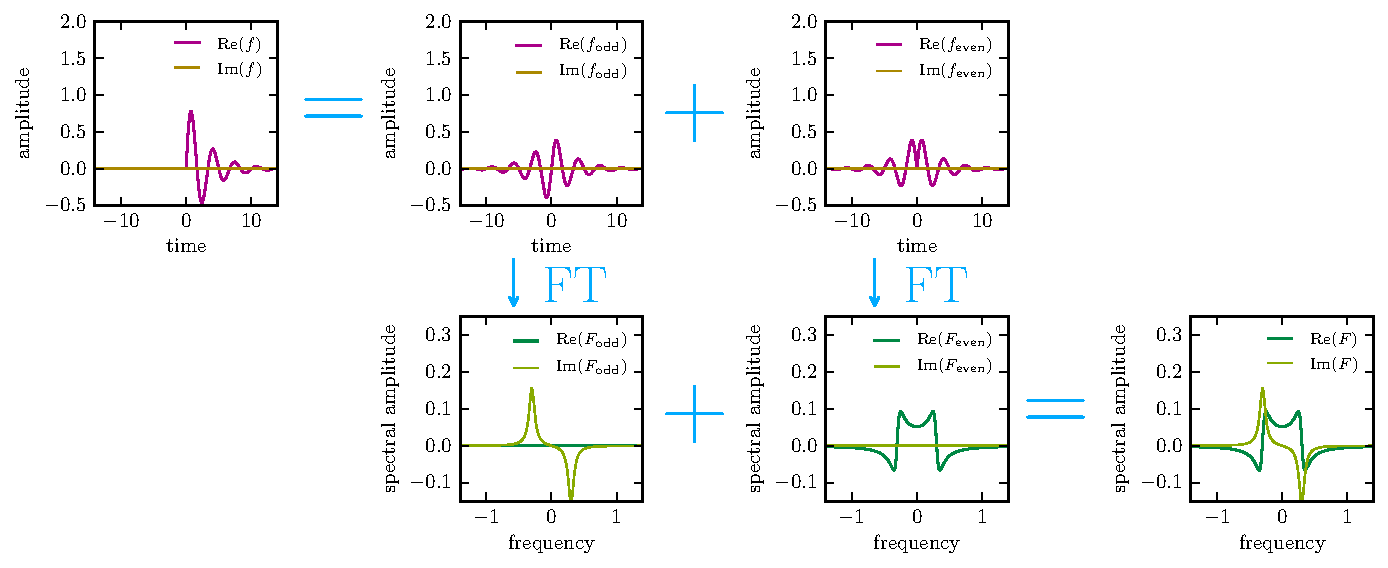
\includegraphics[width=17.5cm]{img/Kramers_Kronig_plot/kk.pdf}
\end{figure}
The Fourier transform of a real odd function is an imaginary function:
%F_{odd}(\omega)=& \int_{-\infty}^{\infty} e^{-\ii \omega t} f(t) \mbox{d}t = \\
		 %=&  \frac{1}{2} \int_{0}^{\infty} e^{-\ii \omega   t } [ f_{odd}(t) + f_{even}(t)] \mbox{d}t 
		   %+ \frac{1}{2} \int_{0}^{\infty} e^{-\ii \omega (-t)} [-f_{odd}(t) + f_{even}(t)] \mbox{d}t  \\
		 %=&  \int_{0}^{\infty} \frac{e^{-\ii \omega t}-e^{+\ii \omega t}}{2} f_{odd}(t) \mbox{d}t 
		   %+ \int_{0}^{\infty} \frac{e^{-\ii \omega t}-e^{+\ii \omega t}}{2} f_{odd}(t) \mbox{d}t  = \\
		 %=&\int_{-\infty}^{\infty} e^{-\ii \omega t} f(t) \mbox{d}t  = \\
		 %=&\int_{-\infty}^{\infty} e^{-\ii \omega t} f(t) \mbox{d}t  = \\
\begin{equation} 
\begin{split} 
F_{odd}(\omega)=& \int_{-\infty}^{+\infty} e^{-\ii \omega t} f_{odd}(t) \,\mbox{d}t = 
		 \int_{-\infty}^{+\infty} \frac{e^{-\ii \omega   t }}{2} f_{odd}(t) \,\mbox{d}t 
		   +  \int_{-\infty}^{+\infty} \frac{e^{-\ii \omega (-t)}}{2} [-f_{odd}(-t)] \,\mbox{d}t  \\
		 =&   \int_{-\infty}^{+\infty} \frac{e^{-\ii \omega t}-e^{+\ii \omega t}}{2} f_{odd}(t) \,\mbox{d}t 
		 = -\ii \underbrace{\int_{-\infty}^{+\infty} \sin(\omega t) \, f_{odd}(t) \,\mbox{d}t}_{\mbox{$\in \mathbb{R}$}},
\end{split} 
\label{eq_kkF}\end{equation}
whereas the Fourier transform of a real even function yields a real function:
\begin{equation} 
\begin{split} 
F_{even}(\omega)= \ldots =   \int_{-\infty}^{+\infty} \frac{e^{-\ii \omega t}+e^{+\ii \omega t}}{2} f_{even}(t) \,\mbox{d}t 
		 = \underbrace{\int_{-\infty}^{+\infty} \cos(\omega t) \, f_{even}(t) \,\mbox{d}t}_{\mbox{$\in \mathbb{R}$}}.
\end{split} 
%% TODO the following is WRONG! see ---->  http://www.thefouriertransform.com/pairs/step.php#signum,  ho3.pdf
\label{eq_kkFeven}\end{equation}
The odd and even components of the time-domain response function correspond to the imaginary and real part of the response spectrum, respectively:
\begin{equation} F_{odd}(\omega) + F_{even}(\omega) = F(\omega), \text{ where } F_{odd}(\omega) = F''(\omega) \text{ and } F_{even}(\omega) = F'(\omega).  \label{eq_kkFodd}\end{equation}
At the same time, $f_{even}(t)$ and $f_{odd}(t)$ are related by having the opposite sign for $t<0$ and the same sign for $t>0$, that is 
\begin{equation} f_{even}(t) = \mbox{sign}(t)\,f_{odd}(t). \label{eq_kkfeven}\end{equation}
Multiplication in the time domain manifests as a convolution in frequency domain
\begin{equation} 
F_{even}(\omega) = \int_{-\infty}^{+\infty}  \frac{-2\ii}{\omega - \Omega} F_{odd}(\omega) \,\mbox{d}\Omega  \equiv  \left[\frac{-2\ii}{\omega}\right]\,\ast\,F_{odd}(\omega),
\label{eq_kkresult}\end{equation} 
where we used the knowledge that the $-2\ii/\omega$ function is the Fourier transform of $\mbox{sign}(t)$. Convolution with this function is also known as the Hilbert transform.% tODO cite

Obviously, Eq. (\ref{eq_kkfeven}) can also be converted to $f_{odd}(t) = \mbox{sign}(t)\,f_{even}(t)$, thus the relation between the real and imaginary part of the response spectrum also holds when $F_{odd}(\omega)$ and $F_{odd}(\omega)$ are exchanged in Eq. (\ref{eq_kkresult}). 

A related mathematical proof of Kramers-Kronig relations can be derived from the analyticity of the response function in the complex plane of frequency. %% TODO cite

%% TODO: why do K-K relations forbid to choose arbitrary phase difference over an unit cell? 
%% ie. Why the Neff can be unambiguously extracted from spectra?
% TODO show how it dictates the "constant area of imaginary part " when resonance Q is changed
%}}}

\subsection{Dispersion relations in local Drude-Lorentz media} \label{disp_rel_local_media}
\paragraph{Lower and upper polariton branches of transverse waves}  % TODO%{{{
Returning to the derivation of dispersion relations, we start with modifying the constitutive relation (\ref{eq_ce}) to a plane wave propagating in a medium:
\begin{equation}		\D := \varepsilon_0\varepsilon_r(\omega)	\E, \quad\quad\quad						\B := \mu_0\mu_r(\omega)		\HH,				 \label{eq_ce2}\end{equation}
with the relative permittivity $\varepsilon_r(\omega)$ and permeability $\mu_r(\omega)$ being two dimensionless functions of frequency, defined in Eq. (\ref{eq_lorentz_eps}, \ref{eq_lorentz_mu}). 
The wave equation (\ref{eq_wavek}) then changes to
\begin{equation} - \kk (\kk \cdot \E) + k^2 \E = \varepsilon_0 \epsrl(\omega) \mu_0 \murl(\omega) \omega^{2} \E, \label{eq_wavek_disp} \end{equation}
which, in the isotropic case, results in the dispersion curve for the transverse electromagnetic wave 
\begin{equation} k~= \sqrt{\varepsilon_0 \mu_0} \sqrt{\varepsilon_{r}(\omega) \mu_{r}(\omega)}\;\omega = \sqrt{\varepsilon_{r}(\omega) \mu_{r}(\omega)}\; \frac{\omega}{c}, \label{eq_dispeq_vac}\end{equation}
with the added frequency-dispersive term responsible for the deviation from the original light line in Fig. \ref{fg_dispersion_vacuum}. 

%TODO FIGURE dispersion curve - scan over resonator strength\\
In the simplest example of a single electric resonance with negligible losses, as in Fig. \ref{fg_dispersion_polariton} % TODO red? line
, the curve is divided into two separate branches. The \textit{lower polariton branch} is below the resonance frequency $\omega_0$ and is characterized by the Lorentz oscillator being in phase with the electric field.
Above $\omega_0$, the dipoles of the Lorentz oscillator can no more follow the electric field and are opposite to it, thus the response of the medium is negative. With further increase of the frequency, the permittivity crosses zero at the frequency $\omega_{\text{L}}$. %, > \omega_0 which allows the transverse wave to propagate. 
where the \textit{upper polariton branch} starts. In case of a Lorentz oscillator unaffected by the presence of others, the difference $\omega_{\text{L}} - \omega_0$ can be computed from the magnitude of the oscillator (using the Lydanne-Sachs-Teller relation).\cite{klingshirn2007semiconductor}

The same behaviour is observed for a single resonance in the permeability $\mu_r(\omega)$, and will be typical also for the spectra of resonances of macroscopic structures described later.

Note that the formation of upper and lower polariton branches can be reinterpreted\cite{landau1984electrodynamics} using the theory of coupled oscillators as the result of \textit{anticrossing} between the oscillator at the frequency $\omega_0$ (forming a horizontal line) and the photon branch (forming a straight growing light-line).

When losses are present, the lower and upper polariton branches are connected by a smooth line of \textit{anomalous} dispersion and very high losses.  % TODO \ref{fg_dispersion_polariton}
%}}}
\paragraph{Longitudinal waves in dispersive media} %{{{
The wave equation in dispersive media, 
\begin{equation} - \kk (\kk \cdot \E) + k^2 \E = \varepsilon_0 \epsrl(\omega) \mu_0 \murl(\omega) \omega^{2} \E, \tag{\ref{eq_wavek_disp} \again} \end{equation}
also allows the existence of longitudinal waves with electric field parallel to the wave vector $\E || \kk$. It was shown earlier that there is no solution for longitudinal waves in vacuum except for static homogeneous field.

If a local medium is assumed, and the wavenumber $k$ is nonzero, such waves can have a solution with nonzero $\E$ when either $\varepsilon_r(\omega)' = 0$, or $\mu_r(\omega)' = 0$. Therefore, the corresponding dispersion curve for a longitudinal wave is a horizontal line at $\omega = \omega_{\text{L}}$, independent of $k$. This would be equivalent to a standing oscillation that maintains the spatial amplitude envelope that was originally excited. 

Different physical phenomena can lead to $\varepsilon_r(\omega)' = 0$, some of which introduce relatively low losses at the corresponding $\omega_{\text{L}}$; namely lattice vibrations in nonconductive crystals or electrons in inductive media (like metals and dilute plasma). At the interface of such media with vacuum or air, another type of waves can be excited with an intermediate frequency $\omega < \omega_{\text{L}}$ that can not propagate in either of the bulk medium. The dispersion curve of such waves is not flat, allowing them to propagate along the interface.
Depending on the mechanism, they are known as \textit{surface phonon-polaritons} or \textit{surface plasmons}, respectively. 
% Are there surface magnons?
% Are there any metamaterials designed for longitudinal waves?
%}}}
\paragraph{Anisotropy of permittivity} \label{par_anisotropy} %{{{
It shall be noted here that permittivity $\epsrl$ was introduced as a scalar, assuming that the vector of electric field $\E$ and electric induction $\D$ are always of the same orientation:
\begin{equation} \D = \varepsilon_0 \epsrl(\omega) \E \equiv \varepsilon_0  
	\left(\begin{array}{ccc} 
			\epsrl(\omega) & 0 & 0  \\
			0 & \epsrl(\omega) & 0  \\
			0 & 0 &\epsrl(\omega)  
	\end{array} \right) \cdot \E
	\label{eq_}
\end{equation}
In some media of lower rotational symmetry (such as many crystals, or liquids under static electric field), the medium response depends on the electric field direction. At the beginning of the chapter, however, we imposed the requirement of \textit{linearity} of the medium. Whatever the linear relation of 
$$\D := \mathcal{L}(\E)$$
is, it must obey the rule
$$\D_1 + \D_2 = \mathcal{L}(\E_1) + \mathcal{L}(\E_2) = \mathcal{L}(\E_1 + \E_2)$$
for any vectors $\E_1, \E_2$. Such a relation can be fully described by a \textit{tensor of permittivity} % TODO cite 
\begin{equation} \D = \varepsilon_0 \epsrl(\omega) \E \equiv \varepsilon_0  
	\left(\begin{array}{ccc} 
	{\epsrl}_{11}(\omega) & {\epsrl}_{21}(\omega) & {\epsrl}_{31}(\omega)  \\
	{\epsrl}_{12}(\omega) & {\epsrl}_{22}(\omega) & {\epsrl}_{32}(\omega)  \\
	{\epsrl}_{13}(\omega) & {\epsrl}_{23}(\omega) & {\epsrl}_{33}(\omega)  
	\end{array} \right) \cdot \E.
	\label{eq_epstensor}
\end{equation}
Elaborate discussion on the restrictions on this tensor and its physical interpretation can be found e.g. in \cite[pp. 678--686]{born1999book}. An analogous treatment can be applied to the magnetic permeability, though it is much less commonly needed.
%}}}
\paragraph{Anisotropic local media}  % TODO%{{{
If the medium response depends on the direction of the field, the dispersion relations can not be directly obtained by substitution into the wave equation. 
It is important to notice that also the leftmost term in 
\begin{equation} - \kk (\kk \cdot \E) + k^2 \E = \varepsilon_0 \epsrl(\omega) \mu_0 \murl(\omega) \omega^{2} \E, \tag{\ref{eq_wavek_disp} \again} \end{equation}
is a linear transformation of the vector $\E$, expressed by the tensor
$$ - \kk (\kk \cdot \E) \equiv 
	-\left(\begin{array}{c} k_x \\ k_y \\ k_z \end{array} \right) \cdot
	\left[\left(\begin{array}{ccc} k_x & k_y & k_z \end{array} \right) \cdot
	\left(\begin{array}{c} E_x \\ E_y \\ E_z \end{array} \right)\right] 
		\equiv
	\left(\begin{array}{ccc} -k_x^2 & -k_x k_y & -k_x k_z \\ -k_y k_x & -k_y^2 & -k_y k_z \\ -k_z k_x & -k_z k_y & -k_z^2 \end{array} \right) \cdot  
	\left(\begin{array}{c} E_x \\ E_y \\ E_z \end{array} \right),
	$$
%$$ k^2 \E \equiv 
%	\left[\left(\begin{array}{ccc} k_x & k_y & k_z \end{array} \right) \cdot 
%	\left(\begin{array}{c} k_x \\ k_y \\ k_z \end{array} \right)\right] \cdot 
%	\left(\begin{array}{c} E_x \\ E_y \\ E_z \end{array} \right),
%	$$
%$$ \mu_0 \varepsilon_0 \omega^{2} \E \equiv 
%	\left(\begin{array}{ccc} k_x^2+k_y^2+k_z^2 & 0 & 0 \\ 0 & k_x^2+k_y^2+k_z^2 & 0 \\ 0 & 0 & k_x^2+k_y^2+k_z^2 \end{array} \right) \cdot  
%	\left(\begin{array}{c} E_x \\ E_y \\ E_z \end{array} \right),
%	$$
The dispersion relation can be reformulated \cite[pp. 667]{born1999book} as a set of linear algebraic equations. 
For simplicity, let us assume the relative permeability $\murl = 1$; then it can be expressed as 
\begin{equation} \det\left[\left(\begin{array}{ccc} 
	k_y^2+k_z^2  	& -k_x k_y 		& -k_x k_z \\ 
	-k_y k_x 		& k_x^2+k_z^2	& -k_y k_z \\ 
	-k_z k_x 		& -k_z k_y		& k_x^2+k_y^2
	\end{array} \right)
-
	\mu_0 \varepsilon_0 \omega^2
	\left(\begin{array}{ccc} 
	{\epsrl}_{11}(\omega) & {\epsrl}_{21}(\omega) & {\epsrl}_{31}(\omega)  \\
	{\epsrl}_{12}(\omega) & {\epsrl}_{22}(\omega) & {\epsrl}_{32}(\omega)  \\
	{\epsrl}_{13}(\omega) & {\epsrl}_{23}(\omega) & {\epsrl}_{33}(\omega)  
	\end{array} \right) \right] = 0, \label{eq_dispdet}\end{equation}
%\begin{equation} \left|\begin{array}{ccc} 
	%k_y^2+k_z^2 - \mu_0 \varepsilon_0 \omega^{2} 		& -k_x k_y 		& -k_x k_z \\ 
	%-k_y k_x 		& k_x^2+k_z^2-\mu_0\varepsilon_0\omega^{2} 		& -k_y k_z \\ 
	%-k_z k_x 		& -k_z k_y		& k_x^2+k_y^2-\mu_0\varepsilon_0\omega^{2}
	%\end{array} \right| = 0, \label{eq_dispdet}\end{equation}
A solution of Eq. \ref{eq_wavek} can exist with nonzero $\E$ if the determinant of the set of three linear equations is zero.
In the most general case, it can be solved by means of numerical algebra software. 
\mdf{
TODO FIGURE: IFC for anisotropic media (are common in nature)\\

TODO FIGURE: IFC for Hyperbolic media (can also be found in nature, in narrow range like near sapphire LO phonno, cite Agranovich)\\
}
%}}}
\paragraph{Isofrequency contours}  % TODO%{{{
%A resonance in local permittivity (or permeability) creates two polariton branches -- thus the dispersion curves can not be expressed as one simple function $\omega(k)$ of the wavevector $k$. It would then appear adequate to treat dispersion curves as a function of frequency, $k(\omega)$, but as is shown below in the presence of nonlocal response, neither $k$ is necessarily a simple function of $\omega$. Also 
It is often important to describe the dispersion curves also for different wave angles, which is the best accomplished by plotting the  %% todo ...real part of ...
frequency $\omega$ as the function of \textit{wave vector} $\kk$. In three dimensions, this would require mapping a function of three independent variables, $\omega(\kk) = \omega(k_x, k_y, k_z)$. However, in most cases the projection of two selected components of $\kk$ is sufficient to understand all relevant phenomena, and naturally it is much easier to visualize.
Such a plot is known as \textit{isofrequency contours} (IFC), or also \textit{equifrequency contours} (EFC). It not only displays rich %?
information about the medium interaction with electromagnetic waves, but also allows for intuitive geometrical analysis of various physical problems. 

The limitation is, however, that IFC plots do not show the imaginary part and thus are applicable to plot dispersion in media with negligible losses only.  % TODO confusing
Each branch also has to be plotted separately, to prevent the contours from overlapping.

\mdf{
TODO FIGURE circular/elliptical/hyperbolic dispersion contours
%% note this is shown in \cite[p. 118]{shalaev2010book}
}
%}}}
\paragraph{Index of refraction, and its applicability}  % TODO%{{{
\mdf{
Noether theorem ->\\
refraction between two isotropic media must keep the phase along boundary   ->  \\
how Snell's arcsin law simply comes out of IFC shape\\

develop the term of index of refraction\\
when does index of refraction make sense? --- strict definition (circular IFC only), weaker definition (tangential and smooth IFC,  works in the limit of small angles, but the beam propagation is not correctly predicted), broadest definition ($k/c\omega$ does not guarrantee prediction of the refraction angle, unusable)

IFCs will be useful also for nonlocal and periodic media later\\


if the surface is smooth, this must hold for any type of media, including anisotropic\\

TODO FIGURE refraction of two media, rgb contours with dispersive angle of refraction
}

%}}}
\paragraph{Phase velocity and group velocity near single resonance}  % TODO%{{{
\mdf{
the discussion regards partial derivative of k-vector by frequency,   d k/d omega ->  \\
derivative of vector function yields another vector function -> \\
show that its magnitude determines the envelope  propagation velocity  \\
and direction determines the beam propagation\\
TODO FIGURE: of this

illustrate the walk-off in a beam \\
TODO FIGURE: beam refraction
TODO move later: show that nonlocal/photonic media can lead e.g. to "beam collimation" when ifc goes flat

show that "signal propagation velocity" is a problematic term <- \\
as a finite-support function spans over infinite spectrum, where group velocity has to change and differ \\
-> "group velocity dispersion (GVD)" leads to signal "chirping" distortion\\
TODO FIGURE: of this

show that near a single resonance, the phase velocity can drop -> \\
group velocity can be negative\\
this happens only in presence of high absorption \cite{mikki}\\
TODO FIGURE: a) eps resonant, mu constant     b) N positive, but group velocity dropping
}
%}}}
\paragraph{Negative phase velocity of doubly-resonant media}  % TODO%{{{
\mdf{
% TODO 0401 how can one tell apart negative refraction due to eps-mu and "nonlocality"?    or shall "nonlocality" just refer to quadrupoles etc?

(here first cite Veselago, not earlier, not later, note that Veselago68 speaks about a truly *homogeneous* medium)\\

*singly resonant media -> positive phase velocity, negative group velocity, this happens near resonance so there are always high losses\\
*doubly resonant media -> negative phase velocity, positive group velocity, above resonant frequencies - theoretically arbitrarily small losses\\
*nonlocal media -> weird things happen, todo\\

TODO FIGURE: a) eps resonant, mu constant     b) N positive, but group velocity dropping

}
%}}}
\paragraph{Energy and Poynting vector}  % TODO%{{{
\mdf{
Poynting vector usually coincides with the group velocity\\

phase velocity is often higher than speed of light, this is no problem\\

cite Mikki for that the Poynting vector \\
}
%}}}

\subsection{Nonlocal response} % TODO
\paragraph{Definition of nonlocal media}%{{{
%TODO: spatial dispersion describes one specific sort of nonlocal behaviour that exists in homogeneous infinite media only
The previous two chapters that concerned local media were included mostly for a comparison with the nonlocal theory that follows.
In this section a more general class of media is discussed, where the polarization explicitly depends the history of $\E(\tau, \brho)$ in previous time $\tau < t$ and in all surrounding points $\brho$, and therefore is described by a spatio-temporal convolution:
\begin{equation} \D(t,\rr) = \varepsilon_0 \E(t,\rr) + \varepsilon_0\int_{V} \int_{-\infty}^{t} \chi_e(t-\tau, \rr-\brho) \, \E(\tau,\brho) \,\mbox{d}\tau \,\mbox{d}^3\brho. \label{eq_chi_convol_nonloc}\end{equation}
In a very similar manner as in the local theory above, we expect a plane wave $\E(t, \rr) := \E_0 \, e^{\ii\omega t - \ii\kk\cdot\rr}$ propagates through the medium. 
\begin{equation} \D(t,\rr) = \varepsilon_0 \E_0 \, e^{\ii\omega t - \ii\kk\cdot\rr} + \varepsilon_0\int_{V} \int_{-\infty}^{t} \chi_e(t-\tau, \rr-\brho) \, \E_0 \, e^{\ii\omega \tau - \ii\kk\cdot\brho} \,\mbox{d}\tau \,\mbox{d}^3\brho. \label{eq_chi_convol_harm_nonloc}\end{equation}
After two  substitutions, $T:=t-\tau$, $\mathbf{R}:=\rr-\brho$, the exponent can again be separated into the original plane wave (which factors out), and a spatio-temporal Fourier transform of the medium response:
$$				 \D(t,\rr) = \varepsilon_0 \E_0 \, e^{\ii\omega t - \ii\kk\cdot\rr} + \varepsilon_0\int_{V} \int_{-\infty}^{0} \chi_e(T, \mathbf{R}) \, \E_0 \, e^{\ii\omega (t - T) - \ii\kk\cdot(\rr - \mathbf{R})} \,\mbox{d}T \,\mbox{d}^3\brho,$$
$$				 \D(t,\rr) = \varepsilon_0 \E_0 \, e^{\ii\omega t - \ii\kk\cdot\rr} + \varepsilon_0\left( \int_{V} \int_{-\infty}^{0} \chi_e(T, \mathbf{R})  \, e^{-\ii\omega T + \ii\kk\cdot \mathbf{R}}\,\mbox{d}T \,\mbox{d}^3 \mathbf{R} \right) \E_0 \, e^{\ii\omega t - \ii\kk\cdot\rr}.$$
The response of the medium to the electric field of any harmonic plane wave can now be expressed as a function of frequency $\omega$ and wave vector $\kk$. It is defined as the ratio between the electric displacement and the electric field:
\begin{equation} \varepsilon_r(\omega, \kk) = \frac{\Dsd(t,\rr)}{\varepsilon_0 \E(t,\rr)} \biggr|_{\E(t, \rr) := \E_0 \, e^{\ii\omega t - \ii\kk\cdot\rr}} = 1 + \int_{V} \int_{-\infty}^{0} \chi_e(T, \mathbf{R}) \,e^{-\ii\omega T + \ii\kk\cdot \mathbf{R}} \,\mbox{d}T \,\mbox{d}^3\mathbf{R} \label{eq_eps_nonloc}\end{equation}
%% TODO think over - we substituted Dsd for D    and    eps for eps^(Loc) , but the new epsilon is not that one containing magnetic effects as in Landau-Lifshitl.
%%	 We must tell apart eps and eps^LL
%%						... should not the notation be unified for clarity? 
%%						... and when it happens that eps == eps^(Loc) ?? And when eps^LL== eps^(Loc)
Converting the problem from spatio-temporal domain into the wavenumber-frequency domain allows to express the relation between $\D$ and $\E$ by the \textit{permittivity} function $\varepsilon(\omega, \kk)$ and completely avoid the convolution from Eq. (\ref{eq_chi_convol_harm_nonloc}). Note that both the response function $\chi_e$ and the permittivity $\varepsilon$ %% TODO make it \varepsilon_r
may be either scalar functions, or rank-2 tensor functions; the latter case accounts for possible anisotropy of the medium.
% , and convolution in space is equivalent to multiplication  in the reciprocal space

The terms of \textit{nonlocality} and of \textit{spatial dispersion} are used interchangeably in the literature. The difference seems to be related to the way one thinks about the medium -- while \textit{nonlocality} is obviously related to the description in the real space (cf. Eq. (\ref{eq_chi_convol_nonloc}), \textit{spatial dispersion} derives from that the response is not a constant function in the reciprocal $\kk$-space. In the author's view, the term \textit{spatial dispersion} is therefore of slightly narrower meaning, as it implies that a plane wave in infinite medium is considered.
%}}}
\paragraph{Local response as a limiting case of the nonlocal one} %{{{
Note the response function for a local medium can be formally derived from its nonlocal formulation by replacing the spatial dependence by a Dirac delta function: %% TODO fix the sencence - it is in fact incorrect
\begin{equation} \chi_e(t-\tau, \rr-\brho) = \delta^{3}(\rr-\brho) \; \chi_e^{\rm(Loc)}(t-\tau), \label{eq_loc_chi}\end{equation}
which allows to simplify Eq. (\ref{eq_chi_convol_nonloc}) in the way that in local media only the temporal convolution has to be computed.

% TODO The exact shape of $\varepsilon(\omega, \kk)$ will be discussed later.
%}}}
\paragraph{Review of local medium parameters}%{{{
Some phenomena observed in the frequency spectrum are in fact consequences of spatial dispersion, such as Doppler broadening of resonance lines in gases.\cite[p. 359]{landau1984electrodynamics} More precisely, these phenomena are primarily dependent on the wave vector $\kk$, and their expression by means of the temporal spectrum is a mere approximation based on that the dispersion curve usually defines a simple relation between  frequency and wave vector. 

The above chapter \ref{disp_rel_local_media} presented the customary approximation of local media, where the electric permittivity in Eq. (\ref{eq_eps_loc}) is composed of two terms: 
\begin{enumerate}
 \item{one caused  by the immediate response of vacuum,} 
 \item{and another by the electric response of matter.}
 \end{enumerate}
In a very similar way, the local magnetic permeability $\murl(\omega)$ also consists of two different components, 
\begin{enumerate}[resume]
 \item{the magnetic response of vacuum,} 
 \item{and, if present, the magnetic response of the matter.} 
\end{enumerate}
\begin{table}[ht]   \caption{Physical effects by the quantity they are expressed by}  \label{tb_nonlocaleff} \centering 
\begin{tabular}{lcr}
 \toprule
Physical effect & Has corresponding term in \\
 \hline
Vacuum permittivity &	&	\\
 &	&	\\
Vacuum permeability &	&	\\
 &	&	\\
 \bottomrule
 \end{tabular} \end{table}


The trivial extension of the local medium description to the nonlocal one could consist in redefining both constitutive parameters as functions of frequency and wave vector: $\varepsilon_r(\omega) \stackrel{?}{\rightarrow} \varepsilon_r(\omega, \kk)$, $\mu_r(\omega) \stackrel{?}{\rightarrow} \mu_r(\omega, \kk)$, but this will not be used. 

% TODO add böhne nägerl reker ulbrich: evidence of spatial dispersion in the dielectric response of continuum states in gaas, 183e WE-Heraeus-Seminar nonlin opt and excit kinetics, noeks, graal-muritz 1997, Germany
%}}}
\paragraph{Magnetic effects can be described by electric displacement}%{{{
%% TODO write about "EDB model"
Instead, we will show here that the magnetic response can be fully expressed by a certain form of $\varepsilon_r(\omega, \kk)$ dependence on $\kk$. In the following theory, the spatial-dispersive function $\varepsilon_r(\omega, \kk)$ will consist of
\begin{enumerate}
 \item{the component caused by the immediate electric response of vacuum,} 
 \item{the component caused by the electric response of matter,}
 \item{and a new component fully accounting for the \textit{magnetic} response of matter, thanks to a particular shape of its spatial dispersion.}
\end{enumerate}
The magnetic permeability $\mu_r$ becomes a mere constant of
\begin{enumerate}[resume]
 \item{the magnetic response of vacuum [as in Eq. (\ref{eq_ce})].} 
\end{enumerate}
Additionally, the spatial dispersion allows to describe
\begin{enumerate}[resume]
 \item{other phenomena that can not be described by the local theory.} 
\end{enumerate}
Repeating the Maxwell equation (\ref{eq_me4}) that links the magnetic field $\HH$ with the electric induction $\D$, 
\begin{equation} \nabla \times \HH =  \frac{\partial \D} {\partial t}, \tag{\ref{eq_me4} \again} \end{equation}
it is clear that if one defines new pair of vector fields
\begin{equation} \HHsd = \HH + \frac{\partial\mathbf{X}}{\partial t}, \label{eq_HHsd}\end{equation}
\begin{equation} \Dsd  = \D  + \nabla\times \mathbf{X}, \label{eq_Dsd}\end{equation}
then Eq. (\ref{eq_me4}) maintains exactly the same form with the new fields, for any differentiable vector field $\mathbf{X}$:
\begin{equation} \nabla \times \HHsd = \nabla \times \HH + \left(\nabla\times \frac{\partial\mathbf{X}}{\partial t}\right) = \frac{\partial \D}{\partial t}+ \frac{\partial(\nabla\times \mathbf{X})}{\partial t} =  \frac{\partial \Dsd} {\partial t}, \label{eq_me4sd} \end{equation}
because for well behaved functions the temporal and spatial derivatives commute.

With the freedom of choice of $\mathbf{X}$, we impose the above mentioned requirement that whole magnetic response of the matter is expressed by the constitutive equation for permittivity. Therefore in spatial-dispersive theory, the constitutive equation %% TODO reference some text from above pargraphs
for magnetic induction is defined the same as in vacuum:
\begin{equation} \mu_0 \HHsd := \mu_0 \murl \HH = \B. \label{eq_mu_sd}\end{equation}
When this equation is rearranged into the form similar to \ref{eq_HHsd}, we obtain a prescription for sought $\mathbf{X}$: 
$$ \HHsd = \HH + (\murl -1)\HH = \HH + \underbrace{\left(\frac{\murl-1}{\mu_0\murl}\right)\B}_{=:\,\partial\mathbf{X}/\partial t}$$
Without loss of generality, we again restrict the discussion to a plane wave (\ref{eq_pw}), thus the time derivative equals to multiplication by $\ii\omega$.
\begin{equation} \mathbf{X} = \frac{1}{\ii\omega}\left(\frac{\murl-1}{\mu_0\murl}\right)\B = \frac{1}{\ii\omega\mu_0}\left(1 - \frac{1}{\murl}\right)\B. \label{eq_Xsd}\end{equation}
The new electric displacement $\Dsd$ that also accounts for magnetic phenomena is obtained by substitution of Eq. (\ref{eq_Xsd}) into Eq. (\ref{eq_Dsd}):
\begin{equation} \Dsd := \D - \ii\kk\times \mathbf{X} =  \D - \ii  \frac{1}{\ii\omega\mu_0}\left(1 - \frac{1}{\murl}\right) \kk\times \B  \label{eq_Dsd2}\end{equation}
By means of the other Maxwell equation (\ref{eq_me3}), the magnetic induction $\B$ can be substituted by $\kk\times\E / \omega$ to obtain an expression that contains the electric quantities only.
\begin{equation} \Dsd = \D - \frac{1}{\omega^2 \mu_0}\left(1 - \frac{1}{\murl}\right) \kk\times(\kk\times \E)  \label{eq_Dsd3}\end{equation}
%}}}
\paragraph{Tensor form of the spatial-dispersive permittivity}%{{{
Continuing in the derivation outlined in \cite{landau1984electrodynamics, krowne2007book_agran, agranovich2006spatial}, we can derive the tensor form of spatial-dispersive permittivity $\varepsilon_{ij}(\omega,\kk)$.

The downsides of the spatial-dispersive model of media is that it is more complicated, leading e.g. to implicit dispersion equation. Its great advantage is however that it provides a correct description of periodic structures discussed below. 
%}}}
\mdf{ TODO REF EBD theory and nonlocal electrodynamics %{{{
\cite{krowne2007book_agran}
\cite{landau1984electrodynamics}
\cite{agranovich2006spatial}
\cite{mikki2009electromagnetic}
\cite{vinogradov2002form}
\cite{golubkov1995boundary}
\cite{agranovich2004linear}
\cite{agranovich1962crystal}
}
%}}}
\paragraph{Speed of light and causality in spatial-dispersive media}%{{{
\mdf{TODO REF Kramers-Kronig relations in nonlocal medium
\cite{skettrup1970kramers}
\cite{kirzhnitz1976}
\cite{melrose1977generalised}
\cite{sun1989kramers}
\cite{rozanov2003}
\cite{bruleanalysis}
\cite{makarov2013kramers}
}%}}}

\subsection{Dispersion relations in homogeneous nonlocal media} % TODO
\paragraph{Comparison of eps-mu and spatial-dispersive models}%{{{
... en vacuum ...
\begin{equation}		\Dsd = \varepsilon_0	\E, \quad\quad\quad						\B = \mu_0			\HHsd,				 \label{eq_ce_dispersive}\end{equation}
%}}}
\paragraph{How a local dielectric manifests in the spatial-dispersive model}  % TODO%{{{
 %(electric quadrupoles..., [Merlin])
%}}}
\paragraph{Why magnetic resonances do not contribute to static permeability?}%{{{
\add{and why high-frequency diamagnetism does not break causality? cite [skaar2014]}
%}}}
\paragraph{Multiple waves at one frequency and additional boundary conditions}%{{{
%}}}

\section{Electromagnetic waves in periodic structures}
\subsection{Bloch theorem}
%In a given time the wave in a periodic medium takes on the form of Bloch wave (\ref{eq_bloch}): 
 %$\mathbf{E}(\mathbf{r}) = \mathrm{e}^{\mathrm{i}Kz} \cdot \mathbf{u}(\mathbf{r})$, i.e. it is a product of a harmonic \textit{envelope} and a cell-periodic \textit{mode}. Computing the dispersion curves involves computing the envelope wavenumber $K = K(f)$ for each frequency $f$ in the desired spectrum. The information about the mode $\mathbf{u}(\mathbf{r})$ is not used and instead the metamaterial cell is treated as if it was a homogeneous medium -- therefore this procedure is also called \textit{homogenisation}.

\paragraph{The Bloch-Floquet theorem}%{{{
% TODO define periodicity

The important Bloch-Floquet theorem states that while the wave in periodic medium does not have to be periodic anymore, it is a product of two periodic functions:
\begin{equation} \E(t, \rr) = \mathrm{e}^{\mathrm{i} Kz - 2\pi \mathrm{i} f t} \cdot \mathbf{u}(\rr), \text{ where } \mathbf{u}(\rr) = \mathbf{u}(\rr+a\mathbf{z}) = \mathbf{u}(\rr+2a\mathbf{z}) = \ldots, \label{eq_bloch}\end{equation} 
The $\mathbf{u}(\rr)$ function has the same periodicity as the structure. It is generally a complex vector function so it not only alters the direction and magnitude of $\E$ (or  $\HH$), but can also introduce a \textit{phase modulation} of the wave in each unit cell. Note that the capital $\KK$ is used to distinguish the wave vector of the Bloch wave envelope from the wave vector $\kk$ in free space. Note this theorem does not determine how the shape of $\mathbf{u}(\rr)$ nor the direction and magnitude of $\KK$, it only states they do exist.
% TODO proof /home/filip/PhD/Sources_MM_theory/Bloch_Theorem_Proof.pdf
% TODO example illustration of Bloch wave -> plotted in Python

%}}}


\paragraph{Virtual periodicity and ambiguity of the mode function}%{{{
\add{
The simplest "structure" to be started with is surely the empty vacuum with homogeneous $\varepsilon := 1$ and $\mu := 1$. One particularly simple solution of the Maxwell equations in vacuum is the planar wave propagating along the $z$-axis, defined by Eq. (\ref{eq_pw2}).
Let us now introduce virtual periodicity, requiring that the vacuum properties are invariant under discrete translation by an arbitrary length $a$ along the $z$-axis, which naturally holds. The important Bloch-Floquet theorem states that while the wave in periodic medium does not have to be periodic anymore, it is a product of two periodic functions:

In a homogeneous medium, there is a simple \textit{dispersion} relation between the frequency  $f$ and the wavenumber $k$, given as
\begin{equation} f = \frac{ck}{2\pi \cdot n} = \frac{ck}{2\pi \cdot \sqrt{\varepsilon \mu}}. \label{eq_dispersion}\end{equation}
The constant $n = \sqrt{\varepsilon \mu}$ connecting the frequency and wavenumber is the index of refraction.

\begin{figure}[ht] \caption{Folded and unfolded dispersion curves for free space and photonic crystal. The phase difference over an unit cell can be expressed either by the wavenumber $K$ (unfolded plots \textbf{a, b} above), or it can be partially absorbed into the periodic mode function $\mathbf{u}(\rr)$ (folded plots \textbf{c, d} below) } \label{fg_phc} \centering  %% TODO write caption; complement the text to match
	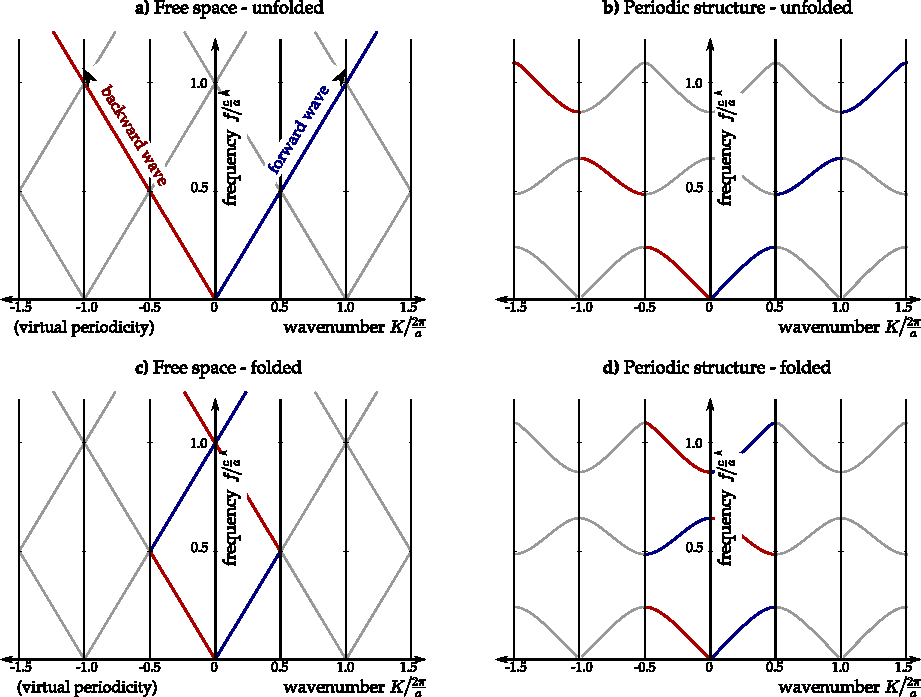
\includegraphics[width=17cm]{img/PhC_folding_illustration.pdf} 
\end{figure}
When the wavelength is less than double cell spacing, or equivalently when $2\pi c /K < 2 a$, the unit cells can scatter the forward propagating wave into the backward direction and vice versa. In an infinite periodic structure the energy transfer must be conserved, so the forward and backward waves must be of the same amplitude.\footnote{The equilibrium forward and backward wave amplitudes may, however, differ in some cases even in in infinite periodic structure. One example is when the constituent materials lose time-reversal symmetry due to static magnetic field.} We assume this also in this example with virtual periodicity. The \textit{Bloch wave} (\ref{eq_bloch}) is a product of two functions, and it gives one degree of freedom to select which part of (\ref{eq_bloch}) expresses the phase shift across one unit cell. Two different conventions are used in the literature.
\begin{enumerate}
 \item{In the \textit{unfolded} plot, the phase shift is expressed entirely by the envelope $\mathrm{e}^{\mathrm{i}Kz}$. One can always find a line coming from the front side of a unit cell to its back side, along which the mode function does not change its phase significantly $\mathbf{u(\mathbf{r})}$. In other words, the volume of the unit cell is not divided by any \textit{nodal plane} in the real part of electric field  $\mathbf{u(\mathbf{r})}$. (However, closed nodal planes within the unit cell may appear due to individual resonances.)

In vacuum, the mode function takes the simplest form, being constant $\mathbf{u(\mathbf{r})} = 1$ at all frequencies. The dispersion relation of vacuum forms a direct line as plot in Fig. \ref{fg_phc}a.} 
 \item{The \textit{folded} plot requires $K/\left(\frac{2\pi}{a}\right) \in (-\frac{1}{2}, \frac{1}{2})$ and the remaining phase is mostly expressed by the mode function. 
Further savings of space in the plot can be made using the symmetry of the forward and backward waves, so only the positive half for $K/\left(\frac{2\pi}{a}\right) \in (0, \frac{1}{2})$ has to be plot to describe the mode structure.} 
 \end{enumerate}
Although maybe less instructive, usually the \textit{folded} bands are plot in the literature and they are used also in Fig. \ref{fg_1dbd}, \ref{fg_rodh} and \ref{fg_erod_radius11} below. The same approach can be used for periodic structures, where the bands are separated by band gaps, cf. Fig. \ref{fg_phc}b and \ref{fg_phc}d.
}
%}}}
\paragraph{Dispersion curves under virtual periodicity}%{{{
The vacuum properties are obviously invariant under discrete translation by an arbitrary length $a$ along the $z$-axis, which can be considered a \textit{virtual} periodicity. 
% TODO mention the terminology "band diagram" - "dispersion curves", is there any real difference?

When the wavelength is less than double cell spacing, or equivalently when $2\pi c /K < 2 a$, the unit cells can scatter the forward propagating wave into the backward direction and vice versa. In an infinite periodic structure the energy transfer must be conserved, so the forward and backward waves must be of the same amplitude.\footnote{The equilibrium forward and backward wave amplitudes may, however, differ in some cases even in in infinite periodic structure. One example is when the constituent materials lose time-reversal symmetry due to static magnetic field.} We assume this also in this example with virtual periodicity. The \textit{Bloch wave} (\ref{eq_bloch}) is a product of two functions, and it gives one degree of freedom to select which part of (\ref{eq_bloch}) expresses the phase shift across one unit cell. Two different conventions are used in the literature.
\begin{enumerate}
 \item{In the \textit{unfolded} plot, the phase shift is expressed entirely by the envelope $\mathrm{e}^{\mathrm{i}Kz}$. One can always find a line coming from the front side of a unit cell to its back side, along which the mode function does not change its phase significantly $\mathbf{u(\rr)}$. In other words, the volume of the unit cell is not divided by any \textit{nodal plane} in the real part of electric field  $\mathbf{u(\rr)}$. (However, closed nodal planes within the unit cell may appear due to individual resonances.)

In vacuum, the mode function takes the simplest form, being constant $\mathbf{u(\rr)} = 1$ at all frequencies. The dispersion relation of vacuum forms a direct line as plotted in Fig. \ref{fg_phc}a.} 
 \item{The \textit{folded} plot requires $K/\left(\frac{2\pi}{a}\right) \in (-\frac{1}{2}, \frac{1}{2})$ and the remaining phase is mostly expressed by the mode function. 
Further savings of space in the plot can be made using the symmetry of the forward and backward waves, so only the positive half for $K/\left(\frac{2\pi}{a}\right) \in (0, \frac{1}{2})$ has to be plotted to describe the mode structure.} 
 \end{enumerate}
Although maybe less instructive, usually the \textit{folded} bands are plotted in the literature and they are used also in Fig. \ref{fg_1dbd}, \ref{fg_rodh} and \ref{fg_erod_radius11} below. The same approach can be used for periodic structures, where the bands are separated by band gaps, cf. Fig. \ref{fg_phc}b and \ref{fg_phc}d.
%}}}
\subsection{Reciprocal space, Brillouin zones and isofrequency contours}
\subsection{Group velocity, phase velocity and their signs}
%\cite{Mikki}
% -> signal velocity, Group velocity, phase velocity and their signs \cite{Mikki}, group velocity can be negative or superluminal - no problem here?
% -> "Hopping model" -- individual oscillators with frequency more-or-less dependent on boundary conditions 
%			 (Neumann ... Gamma point ... "dE/dx=0"  vs.  Dirichlet ... M-point ... "E=0")
\subsection{Antiresonances and problems with local effective parameters}

%% REF \cite{wallen2010}: Anti-resonant response of resonant inclusions
%  antiresonance "may not" come from periodicity, as it is also in random structures
%% REF \cite{alu2010}: Restoring the physical meaning of MM cosstitutive parameters

% in the following we will plot the unfolded bands instead as it seems to give clearer physical interpretation of data.
% -> TODO doplnit "PhC book": dispersní křivky atd.

\subsection{Properties of photonic band-gaps}
% -> application of PBG, todo add references; formation: \cite{laktionov2008}
% -> zero-width case, as a transition between a mode traversing from one photonic band to another
% -> concept of nodal planes (or, more precisely, surfaces)
% -> exponential wave decay with phase difference across the cell
% -> note about how Fourier transform allows no point source to radiate energy within the bandgap
% -> PhCs with metallic/metamaterial inclusios, [Monsoriu, Lina Shi and friends]
\subsection{Physics of negative phase and/or group velocity media}
% -> homogeneous media with negative group velocity
% -> refraction on the boundary 
% -> negative group velocity and power flow [Mikki]
% -> negative index media
% -> isofrequency contours in DNG


\subsection{Homogenization}
\mdf{
ref Homogenisation issues - response to our paper from OpEx
\cite{rockstuhl2008transition}
\cite{paul2011reflection}
\cite{andryieuski2012bloch}
\cite{andryieuski2010homogenization} 
\cite{simovski2007bloch}
\cite{simovski2009material}
\cite{simovski2011electromagnetic}
\cite{mortensen2010unambiguous}
}
%% "process of replacing a complex structure of subwavelength sized components with an “effective medium” with uni-
%% form properties. It is a fundamentally important notion which can be traced back to the earliest days of electro-
%% magnetic theory, to the Lorentz-Lorenz and Maxwell-Garnet effective medium models [1–3]
%			[1] J. C. M. Garnett, Phil Trans. R. Soc. A 203, 385 (1904).
%			[2] D. E. Aspnes, Thin Solid Films 89, 249 (1982).
%			[3] W. Cai and V. Shalaev, Optical Metamaterials: Fundamentals and Applications (Springer, New York, 2010).

% "Metamaterials do not bring new physical phenomena, they only force one to conscientiously review the common electrodynamics. There
% are no novel phenomena, just a novel task of homogenisation and possibly enew values of constitutive parameters"


\subsection{What are metamaterials and photonic crystals?} %{{{
\add{
%% This is after the theory of eldn in periodic media.
%% Nonresonant metamaterials (ie. in the 1st Brillouin zone, see [Kadlec2008 / Vol. 33, No. 19 / OPTICS LETTERS] and Juraj]
%% resonant metamaterials operate in the 2nd BZ (or possibly even third or higher? )
%% Think over, note the paper Dominec2014

The studies of periodic electromagnetic structures is generally divided into two classes: the \textit{photonic crystals} and \textit{metamaterials}. These types of structures are formally very similar, as they are composed of 2-D or 3-D periodic array of unit cells, and the qualitative difference can be found only after the interaction with an electromagnetic wave is known. 

%The difference is in the way how the unit cell interacts with the electromagnetic field. 
In the photonic crystal (PhC), at its frequency range of operation, the effective wavelength is similar to the cell spacing and the cells scatter the propagating wave.
The energy of the resonant field is spread relatively evenly over the majority of the unit cell volume, which results in great sensitivity of the PhC behaviour to its periodicity and typically also in a high spatial dispersion. The most prominent phenomenon observed in PhC is the emergence of forbidden photonic bands around resonant frequencies, where the light can not propagate through the structure. 

On the contrary, 
the cells of a metamaterial (MM) are expected to exhibit individual resonances which should not significantly couple to each other. 
At the resonant frequencies in the metamaterials, the majority of the energy of the electromagnetic field is localised in a fraction of the unit cell volume, so that the behaviour of the metamaterial usually has only weak spatial dispersion, if any. This allows one to describe many metamaterials with acceptable precision as a homogeneous medium with a index of refraction $N(f)$, wave impedance $Z(f)$ and related effective permittivity $\varepsilon(f)=N/Z$ and permeability $\mu(f)=NZ$. 

Both types of structures exhibit the most interesting behaviour at their frequencies of resonance, but the different types of resonances define the technology and materials used to build them. The resonances in PhC rely on wave scattering, which can be easily obtained with any ordinary low-permittivity material such as silica or silicon. On the other hand, the resonances 
%but the mentioned difference has profound consequences on the behaviour of the structure. 
%}}}

}
\begin{figure} \caption{img/mm-phc-diagram.pdf}  \centering 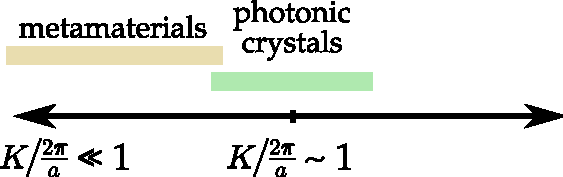
\includegraphics[width=10cm]{img/mm-phc-diagram.pdf} \end{figure} \clearpage
%% MM: HOW the light propagates.  <------>      PhC: IF the light propagates.
%% Definitions:
%% Igor Tsukerman: (Nonlocal homogenization of metamaterials by dual interpolation of fields)
%%   "metamaterials - artificial periodic structures with features smaller than the vacuum wavelength"
%% note that Veselago68 speaks about a truly *homogeneous* medium
% -> cloaking (aside from losses)
% -> superlens (aside from losses and aberration, in a hypothetical case that the MM structure can be made much finer than a detector ...)
% -> hyperlens 
%    The resolution of metamaterials is hindered by their internal cell size, and even sooner, by the spatial dispersion.
%    Hyperbolic metamaterials are commonly thought to be able to form a hyperlens, but the hyperbolic shape of the IFC is only an approximation
%    for low wavenumber; it possibly strongly differs when K~is big, and possibly also forms a closed surface instead of infinite hyperboloids.
% -> metasurfaces (impedance engineering, tunable properties, thin high-contrast filters)
% Losses are in \cite[p. 708]{born1999book}


\paragraph{Historical regards}
\paragraph{Attempt of proper definition of Metamaterials}
%% TODO
%% This is after the theory of eldn in periodic media.
%% Nonresonant metamaterials (ie. in the 1st Brillouin zone, see Juraj]
\cite{richter1995}
\cite{kadlec2008}

More detailed investigation shows that the effective-medium approach does not give accurate results when the structure is not infinite \cite{richter1995}, as is often the case. Therefore, a numerical computation using the rigorous coupled-wave analysis (RCWA) or using FDTD has to be used.

%% note Silveirinha 2007 
%% resonant metamaterials operate in the 2nd BZ (or possibly even third or higher? )
%% Think over, note the paper Dominec2014

%% PK: "The word “metamaterial” (MM) appeared first in the paper by Smith et al. in 2000 [6] where a structured material" -- is it true?

% "note that whenever a transmission is plotted, one always refers to a finite sample; in the discussion of infinite (periodic) media, 
%       only the allowed or forbidden band are to be discussed"



\section{Materials available for metamaterial construction}
\subsection{General notes}
% TODO we refer to tunability - complete it in the rest of the document!!
%% TODO unify impedance as `Z', not `z'
\subsection{Dielectrics}
\subsection{Metals}
% and oxides for optical: Naik2011.pdf
\subsection{Superconductors}
\subsection{Tunable and switchable materials}
\subsection{Specifics of the terahertz range}



%Introduction
	%What is metamaterial
	%Motivation for MM
	%Motivation for THz range
%Fundamentals
%Dielectric spectra
%eps,mu -> N,Z -> reflectivity
%K-K relations
%putting two resonances near to each other annihilates their “wings”
%→ hard to make a broadband-operating passive MM
%Metal eps spectra
%different models: Drude, lossy Drude
%spatial view of E+M wave propagation  (propagating/standing wave)
%in free space
%in arbitrary electromagnetic material 
%reflection on metal surface (PEC) and on PMC
%surface plasmons, standing/propagating
%non-lossy and lossy metal (-> quasi-bound states)
%interpreting resonance (and Fano-resonance) curves
%wave in free space → s12 ampli constant, phase constantly growing; (s11 zero)
%→  in polar plot: a clockwise rotating unit vector
%reflective surface → s11 ampli constant, phase constantly growing; (s12 zero)
%simple resonance (in SRR?) 
%→  reflectivity peak
%→  losses
%in polar plot of s12: fast clockwise curl, approaching zero point, phase up-DOWN-up
%in polar plot of s11: clockwise curl starting at zero, making trip, returning to zero
%Fano resonance: requires spiral segment of curve
%case of "little fast curl 1" on "big slow curl 2"
%if fres1 = fres2 → subtractive effect, both in amplitude and phase; phase up-down-UP-down-up
%if fres1 < fres2 → …
%find out the difference between:
%two coupled broad resonances with interaction inbetween?
%Capacitive, inductive, resistive coupling?
%a “fast” and a “slow” resonance superposed?
%Two oscillators with nearly the same frequency:
%electric+electric or magnetic+magnetic → strong coupling, leads to twice curled curve in polar plot
%electric+magnetic → weak or no coupling (magnetic dipole: H field even, Efield odd; electric dipole: H field odd, E field even → may be regarded as zero inner product of the field functions)
%Scaling and non-scaling properties [Zhou PRL 2005]
%(Mode curve anticrossing)
%Babinet principle
%(Quantum states in left-handed media?)
%
%Building metamaterials: key principles
%Homogenisation
%methods, issues, desired homogenized parameters
%Metal functions
%diluted metal → Pendry1996's low frequency plasmons
%(Are cut-wire stripes useful e.g. for stable numerical simulations? They have finite eps at freq=0)
%antennae: resonator-field coupling
%metallic resonators: negative mu from SRR/Horseshoe/double-stripe
%Bianisotropy and chirality
%SRR and double-SRR
%keeping rotational-translational symmetry
%tunability
%MM impedance and coupling to free-space waves
%Mode coupling
%capacitive/resistive, behaviour, conditions, applications
%relations between MM and photonic crystal
%Higher-order Bloch modes
%
%Selected all-dielectric metamaterials
	%Mie resonances in high-permittivity microspheres
%
%Selected metalo-dielectric metamaterials
	%Aperture-array transmission
		%Wood anomaly in slit arrays
		%Wood anomaly in hole arrays
		%Standing SPP wave
	%“thin wires [8], [28], Swiss rolls [9], SRRs [9], electric SRRs (eSRRs) [29], [30], pairs of rods [10], [12], [31], pair of crosses [32], fishnets [17], [33]”
%
%== Weird ideas to elaborate ==
%* helical wire medium -> higher inductive load -> enables low plasma freq even for thicker wires
	%---> calculate FDTD
	%---> measure   TDTS with light bulb wires!
%* Possibility of standing phonon-polariton on SiC (!) 
%* try the anisotropic magnetic goo from the drawing board for children (but for electrical response)
%* find out how they could achieve negative phase speed
%* quantum point of view to negative phase/group velocity 

\chapter{Experimental and numerical methods}
\section{Short review of the terahertz technology}
The terahertz range of the electromagnetic spectrum, spanning roughly from 100 GHz to 10 THz, has met as yet a relatively small application potential in science and technology in the 20th century, compared to the development in the microwave ($<$ 100 GHz) and near-infrared ($>$ 100 THz) or optical ranges. The reason can be traced down both to the limited choice and high cost of suitable terahertz sources and detectors, and to their usually small efficiency or sensitivity, respectively. The technology and science, however, develops fast in this field, and the number of terahertz-related papers has doubled every 3.2 years \cite{lewis2014review} between 1975 and 2010.  

There is a great number of books and papers that describes different terahertz sources and detectors in detail \cite[pp. 155-158]{lee2008book}\cite{sullivan2012field,lewis2014review}
and many of them are also, with more or less detail, discussed in previous doctoral theses written in our group (\cite[pp. 2-30]{pashkin2004phd}, \cite[pp. 19-25]{nemec2006phd}, \cite[pp. 7-26]{fekete2008phd}, \cite[pp. 11-21]{sibik2010dp}, \cite[pp. 31-45]{yahiaoui2011phd}, \cite[pp. 33-38]{mics2012phd}, \cite[pp. 25-33]{skoromets2013phd}, etc.).

Electromagnetic waves in the terahertz range are radiated whenever charged particles are subject to fast-enough acceleration at the picosecond scale.  The generation processes may be sorted with regards to the medium in which the emission occurs and to the origin of the force causing the acceleration.  In the following paragraphs, we try to briefly review the terahertz technology in a systematic manner.

Firstly, let us remind why thermal sources are rarely used in the THz range, although they are otherwise widely used at higher frequencies. The blackbody radiation is governed by the Planck law % TODO cite
\begin{equation}I(f, T) = \frac{2 h}{\pi^2 c^2}\frac{f^3}{e^{\frac{h f}{kT}}-1} \mathrm{\,W\,sr^{-1}\,Hz^{-1}\,m^{-2}}, \label{eq_planck}\end{equation}
from which it follows that the luminosity $I$ in the terahertz range is always very small: Integrating over frequencies from 300 GHz to 3 THz, one obtains roughly 0.6 W sr$^{-1}$ m$^{-2}$ at the room temperature ($T=$ 300~K).  Furthermore, all Planck oscillators at the frequency of e.g. $f =$ 1~THz are already fully saturated:
%  although the thermal energy at room temperature $T$ is significantly higher than the photon energy $hf$ at 1 THz
$$k_B T \approx 1.38\cdot 10^{-26} \text{ J K}^{-1} \cdot 300 \text{ K~} \approx 25.8 \text{ meV } \quad\gg\quad h f \approx 4.13 \text{ meV}, $$
and therefore the power radiated in the THz range can not be significantly improved by increasing the blackbody temperature. Particularly, it can be shown that in this part of the spectrum the luminosity scales only linearly with the temperature $T$; in contrast, the total power scales as $T^{4}$ as follows from the Stefan-Bolzmann law. Therefore, sources other than thermal are preferred for measurements in the THz range.

\subsection{Terahertz sources}
\paragraph{Kinetic energy of an electron beam} %{{{ ================================================================================
One class of devices uses the kinetic energy of an electron beam propagating in the vacuum. In devices accelerating a circular electron beam, such as cyclotrons or synchrotrons, radiation is emitted when electrons are passing through the bends in the particle path, the deflection of the electrons being caused by a static transverse magnetic field. If the electrons are packed in a short bunch, it results in an efficient emission of a coherent broadband pulse. %% with an improved efficiency in THz if they are packed
Another example is the free electron laser with the electron bunches %% TODO ... forming upon ...
passing through a periodically-poled magnet called \textit{wiggler}. 
Both types of devices provide an excellent brightness and tunability, but they are rather large-scale facilities often with a dedicated building. 
%In both devices, the electrons have to propagate in bunches. 

Tabletop sources of radiation covering a part of the THz range are the microwave vacuum tubes: \textit{gyrotron}, travelling-wave and backward wave oscillators (BWO, also known as \textit{carcinotrons}, of the O- and M-types), and \textit{klystron}. The unifying principle of these devices is that an electron beam speed, position or density can be modulated the electric field, and the modulation in turn radiates amplified electromagnetic wave. Backward-wave oscillators are 
used for continuous-wave spectroscopy, but the tunability of one device is typically limited to tens of percent and the power drops with the frequency \cite{lewis2014review}.
% M-type, the most powerful, (M-BWO) and the O-type (O-BWO). The O-type delivers typically power in the range of 1 mW at 1000 GHz to 50 mW at 200 GHz. 

%}}}
\paragraph{Terahertz solid-state oscillators}%{{{================================================================================
Reducing the size of the active regions of well-established microwave devices, such as microwave diodes, transistors and vacuum tubes, usually enables scaling down the wavelength of the emitted radiation proportionally with the dimensions. 
The fundamental issue lies in that the power drops very fast when the device is miniaturized. If the total emitted power is limited by cooling, i.e. by the surface of the active region, it drops with the second power of the device size. If the volume power density is the determining factor, the power drops even faster.  % TODO examples of dropping power
As a solution, either substantial changes in the device geometry, constituent materials, or even new physical principles have been introduced for efficient THz sources \cite[pp. 8-12]{sullivan2012field}.  

%This concept is, in fact, applicable to all % TODO is this truly 'all'?
 %devices where the wavelength is not determined by quantum phenomena, or by physical quantity other than dimension (such as the magnetic field strength in a magnetron tube).

If a relatively low power is required, principles used in microwave engineering can be extended to the lower part of the terahertz spectrum.  %% TODO stylistics
The frequency range of operation of high-electron-mobility transistors (HEMT) has also been extended roughly up to 1 THz. %Sometimes all accompanying components are integrated to a MMIC.

An oscillator may be formed by placing an element with negative differential resistance (NDR) into a resonant cavity or circuit. 
In \textit{Gunn diodes}, widely used in microwave technology, the NDR is due to the electron effective mass abruptly increasing with their velocity in certain direct-gap semiconductors.
In \textit{resonant tunneling} diodes (RTDs)\cite{asada2008resonant,brown1991oscillations}, NDR is achieved by a heterostructure quantum well, where, upon an increase of the voltage, the electron energy is detuned from the resonance of the quantum well, and the current is reduced.

Yet another principle is employed in the \textit{impact ionization avalanche transit-time} (IMPATT) diodes, where a non-destructive breakdown of a reverse-biased p-n junction follows the voltage with a delay which again enables oscillations if surrounded by a cavity. 
In contrast, in the \textit{tunneling transit-time} (TUNNETT) diodes, the NDR is achieved by changing the transit time of carriers through the semiconductor volume.
%}}}
\paragraph{Nonlinear up-conversion of microwaves}%{{{ ================================================================================
The nonlinear response of semiconductor devices to microwaves can be used for up-conversion into the terahertz range. Starting from a relatively powerful and widely available semiconductor source operating in the 100 GHz range, frequency multiplying stages are are often cascaded to reach frequencies several times higher (e.g. \cite{thomas2012first}). 

Harmonic frequency multipliers and mixers often employ varactor diodes or Schottky diodes embedded in a waveguide. They however still suffer from significant power drop above 1 THz.

%}}}
\paragraph{Nonlinear down-conversion of optical waves}%{{{ ================================================================================
The opposite approach, also known as \textit{optical rectification}, generates THz radiation as the difference frequency between two or more detuned optical waves.
The radiation may come from two lasers or laser modes, % [CCap7], 
mutually detuned by a frequency that is to be generated. %% TODO The lasers may be classical solid state, diodes or e.g. two modes in one infrared QCL. %% TODO cite one classical, and the QCL
Other possibility is to use the \textit{terahertz parametric generation} where a single wave enters the nonlinear crystal as the \textit{pump} and the second wave, \textit{idler}, is generated during the nonlinear process. The \textit{idler} wave is kept in an optical resonator; the terahertz output can be tuned by changing parameters of the resonator. 
For nonlinear generation of pulses in the THz range, usually a mode-locked laser is used that emits pulses that intrinsically cover a broad spectrum of frequencies (e.g. typically over 360-390 THz for a titanium-sapphire laser). The difference-frequencies are generated from all optical frequency components simultaneously, which results in a terahertz pulse with a very broad spectrum given by the type of nonlinear medium. 

The classical process of nonlinear optical conversion involves transparent electro-optic crystals, where some measures are taken to account for the generally different velocity of all interacting waves.
\begin{itemize}
	\item{For the difference-frequency generation between optical waves of close frequency, the classical condition of \textit{phase synchronization} is equivalent to ensure similar \textit{group} velocity at the optical and terahertz frequency. Of the materials satisfying these requirements, zinc telluride (ZnTe), gallium selenide (GaSe), and lithium niobate (LiNbO$_{3}$) % [CCap19]) 
found widest application in the frequency range up to 3--5 THz. } 
\item{The \textit{quasi-phase-matching} technique allows to compensate the difference of the group velocity of the optical wave and the terahertz wave by periodically altering the nonlinear coefficients of a crystal so that the nonlinear contribution to the resulting wave never reverses its sign. Crystals of \textit{periodically poled lithium niobate} (PPLN) are often used for this, with the possibility of shaping the poled regions as wedges (\textit{fanned-out PPLN}), which allows to change the effective poling pitch. This method is suitable for continuous-wave or narrow-band pulse terahertz generation.  }  % TODO cite 
\item{A sufficiently strong nonlinear interaction, on a length less than the coherence length, alleviates both requirements of phase matching and low absorption of the waves \cite{leitenstorfer1999detectors}. Organic crystals, e.g. made of DAST,\footnote{DAST is a shortcut for 4-dimethylamino-N-methylstilbazolium tosylate}
%% and derivatives of MNA (2-methyl-4-nitroaniline) [CCap25]
have been reported \cite{han2000use} %[CCap24]
to have two orders of magnitude higher electrooptic coefficients than the materials usual in nonlinear optics, making them suitable for operation up to 20 THz. 

Nonlinear interaction is semiconductors is enhanced when the incident photon energy is above their band gap. Common crystals used for \textit{resonant THz emission} are GaAs, %[CCap22] 
InP  or CdTe (with band-gaps of 1.42, 1.34 and 1.5 eV, respectively), which can be illuminated by a titanium-sapphire laser (with an average photon energy $hc/\lambda \approx$ 1.5 eV).} 
\item{With a proper spatio-temporal optical pulse geometry and choice of materials,\cite{auston1984cherenkov} a THz pulse can be generated in the form of Čerenkov cone even if the optical group velocity is higher than the terahertz one.}
\item{Finally, plasma generated by high optical intensity of an optical pulse can serve as a nonlinear medium, with a low dispersion and thus a very broad bandwith of tens of THz \cite{loffler2000generation,chen2007terahertz,tong2012}. }
 \end{itemize}
%% TODO Sub-cycle control of terahertz high-harmonic generation by dynamical Bloch oscillations
%% TODO and also http://www.nature.com/srep/2014/140605/srep05045/full/srep05045.html#close

%}}}
\paragraph{Photoconductive sources}%{{{ ================================================================================
Terahertz waves can be generated by \textit{photoconductivity}, i.e. by transient acceleration of charges upon optical illumination.
%In a non-saturated regime, the change of conductivity is roughly proportional to the light intensity, and thus to the square of the electric field amplitude. In this respect, the photoconductivity is similar to the aforementioned mechanism of the second-harmonic nonlinear interaction. 
In the photoconductive devices, the major part of the energy is supplied by the external quasi-static electric field, which limits the maximum emitted power and requires less intense laser illumination. The light sources can be again two detuned lasers or laser modes \cite{gu1999generation}, or a pulse from a mode-locked laser oscillator. Obviously, this method requires the photon energy to exceed the band-gap of the selected semiconductor.

The photoconductive emitter is usually a slab of a suitable semiconductor with the antenna structure, deposited on the illuminated side \cite{auston1984picosecond}. Earlier antenna designs use two metallic segments of different shapes, such as split-H shape or a spiral. The gap between the electrodes may vary; the \textit{large-aperture} emitters with several mm gaps % TODO 
allow to increase the energy and directivity of the THz radiation in the pulsed regime, however they require high-voltage power supply.
The optical beams (continuous or pulsed) are always more or less tightly focused to the gap between the electrodes. 

The \textit{interdigitated emitter} \cite{darrow1990subpicosecond,hu1990optically} 
provides a large-aperture and relatively high-energy THz pulses even with low voltage in the range of tens of volts. The metallisation on its front side forms a dense array of narrow metallic wires; every second gap between them is covered with opaque paint. The odd and even wires are connected to two terminals of a voltage source.  Upon pulsed illumination, all charge stored in the interdigitated electrodes discharges through the illuminated part of the semiconductor surface, emitting a THz wave polarized perpendicular to the wire grid.

The emission efficiency can be improved when the sharp current rise is followed by a similarly sharp falling edge of the current, again in the order of one picosecond. For this purpose one needs to select a material with a very short lifetime of carriers, but a relatively high mobility thereof. Radiation-damaged silicon films on sapphire, or gallium arsenide slabs with lattice disordered either by (Be or Cr) doping, or by growing at low temperature, are used. 

A weaker THz emission can also be observed from semiconductors even with no static bias voltage, owing to the surface electric field, photo-Dember and other phenomena \cite{corchia2001effects, heyman2001terahertz}.
%%% todo understand this more  HN: "surface depletion field in semiconductors can serve for carrier acceleration, avoiding the necessity of using an external voltage source" \cite{liu2003terahertz,zhang1992optoelectronic}
%%%   HN: "several mechanisms responsible for the enhancement depending on the excitation intensity" 

%}}}
\paragraph{Terahertz lasers}%{{{  ================================================================================
Continuous gas terahertz lasers use stimulated emission from quantum transitions between discrete rotation levels of small organic molecules \cite{chang1970cw}. Although they present high-brightness continuous sources at multiple lines in the terahertz range, they are rather expensive and their quantum efficiency is poor, as they usually have to be pumped by a powerful carbon dioxide laser at 33 THz.

Solid-state terahertz lasers are represented by the p-doped germanium laser, where the quantum transition occurs between light and heavy holes in strong magnetic field and at cryogenic temperatures. The transition frequency can be continuously tuned by the magnetic field.

Quantum cascade lasers (QCL) are composed of hundreds of semiconductor layers \cite{yin2012terahertz}, which create multiple closely-spaced quantum levels. Each electron or hole traversing the structure thus undergoes multiple transitions. Such devices are compact and  efficient sources of continuous and slightly tunable radiation in the mid-IR region. The extension of their operation under 2 THz always requires cryogenic cooling and is subject to intense research.
%}}}
\paragraph{Other THz sources}%{{{ ================================================================================
Although a complete list of all physical phenomena that lead to possibly useful emission of terahertz waves is beyond the scope of this thesis, we try to point out some most notable examples of these. 

Earlier in our laboratory it was observed that an oblique impact of femtosecond optical pulse on 50-150 nm thick gold layer on glass emits a THz pulse of similar energy as those from an interdigitated emitter \cite{kadlec2004optical,kadlec2005study}. Other experiments, e.g. with thin organic layers \cite{ramakrishnan2012surface}, suggest the process may be intensified by surface plasmons.

Tunable terahertz continuous-wave emission was observed in multiple stacked Josephson junctions \cite{ozyuzer2007emission}, where the oscillation frequency is determined by the junction voltage as $f(U) = 2e/h$, thus 2 mV correspond to roughly 1 THz. This method however requires cryogenic temperatures as a superconductor structure is used, and is still subject to primary research.

The \textit{Smith-Purcell} effect is observed when relativistic electron beam passes close to a corrugated surface, e.g., of an optical grating. The emitted coherent radiation can be obtained also in the THz region \cite{doucas1992first} (as determined by the grating pitch). A similar effect was later observed from a direct current flowing through a graphene monolayer placed over a photonic crystal \cite{tantiwanichapan2014graphene}.
%% TODO add: GEME coherent?, 
%% TODO add: THz HHG? http://www3.imperial.ac.uk/newsandeventspggrp/imperialcollege/naturalsciences/physics/exssseminars/eventssummary/event_21-10-2014-13-26-55
%}}}

\subsection{Terahertz detectors}
\paragraph{Thermal detection}%{{{
A broad class of detectors, applicable also to the terahertz range, measures the energy of the radiation. 
Classical bolometers use elements that change resistivity (thermistors, thermocouples) when they are heated by radiation.
Pyroelectric detectors convert the heat directly to the electric signal by means of a crystal that changes its polarisation with temperature. In Golay cells, an incident terahertz pulse heats the air, whose thermal expansion is detected. Such devices usually operate at room temperature.

The concept of a bolometer can be greatly improved, in terms of sensitivity or speed, at cryogenic temperatures when a superconductor near its critical temperature or a doped semiconductor are used as the temperature detector. In the \textit{hot-electron} bolometers, the superconductor forms a narrow bridge between two contacts so that the changes in resistance are more pronounced. The changes in the superconductor behaviour can also be detected by a superconducting quantum interference device (SQUID).  

%}}}
\paragraph{Heterodyne mixing}%{{{
Terahertz continuous-wave signal can be mixed with the signal from a local oscillator, producing a difference frequency in the microwave spectral range which can be easily processed using an oscilloscope or a spectral analyzer. The nonlinear components often used up to 1 THz are Schottky diodes or superconducting Josephson junctions \cite{face1986high}.
Fast enough thermal detectors, such as hot-electron bolometers based on Nb or NbN superconducting transition, can also be used with a higher sensitivity \cite{lee2008book}.
 instead of the time-averaged power density.

%}}}
\paragraph{Time-resolved field sampling}%{{{
Another class of terahertz detectors enables measuring the electric field $\E(t)$ [or magnetic field $\HH(t)$] as a function of time. An important advantage of such devices is the possibility to recover the instantaneous amplitude of the field (i.e. both its modulus and phase in the frequency domain). It also allows to synchronize the detection with the pulsed source to record short terahertz transients.
(It should be noted that the measurement of the transmittance phase can be accomplished with continous tunable source, too, using a Mach-Zender interferometer.
Pulsed measurement is however vital for transient dynamics investigation.)

Most of such detectors are based on coincidence of the terahertz pulse and a \textit{sampling} (or, \textit{gating}) optical pulse. The mutual timing of the pulses can be scanned using an optical delay line, thus the terahertz waveform can be recovered over repeated measurements \cite{wu1996ultrafast}.  % ist it appropriate?
Alternatively, various single-shot detection schemes have been also implemented, usually being based on the temporal dilation (chirp) of the sampling optical pulse and subsequent spectral analysis of the output.
% TODO check the THz detectors as I proposed
% HN: In the other configuration the ellipticity is measured near the zero-transmission point (Fig. 1.3b) [hn54]
% HN: this scheme is important when a single photodetector is required, like in certain imaging applications [hn55] or in single-shot measurements [hn56]
The physical process of the optical sampling is in most cases analogous to one of the above described mechanisms of terahertz pulse generation:
\begin{enumerate}
 \item{Photoconductive receiving antennas use a short optical pulse to introduce a subpicosecond time window to short-circuit the antenna segments. The instantaneous THz field at the time of the optical pulse arrival moves a proportional charge across a superconductor gap between two metallic stripes. The voltage difference can then be amplified and measured by relatively slow electronics.} 
 \item{Electrooptic sampling uses the nonlinear interaction between the optical and THz electric field in an electrooptic crystal, typically a thin plate of ZnTe. To discriminate between the sampling optical pulse and the weaker component added to it by the nonlinear interaction, usually a change of optical polarization is detected.}  % todo add that this will be discussed?
 \item{Magnetooptic sampling was also demonstrated \cite{riordan1997free}, based on the Faraday rotation induced by the magnetic component of a transient THz wave.}
 \end{enumerate}
Similar to all cases of the pulsed terahertz sources, the temporal resolution of sampling terahertz detectors is generally limited by the duration of the sampling optical pulse, and more often, by the limited speed of the photoconductive antenna or by group velocity dispersion of the nonlinear crystal. The detection bandwidth can be improved using the approaches used in the terahertz pulsed sources  such as the use of thin plates of organic crystals (DAST) % CITE
or nonlinear detection in plasma.
%% 
%% %TODO about synchronicity - almost always pumped/triggered by a pulsed laser
%% \mdf{
%% "The THz radiation is generated in a large area THz emitter"
%% %\cite{12   A. Dreyhaupt, S. Winnerl, T. Dekorsy, and M. Helm, “High-intensity terahertz radiation from a microstructured large-area photoconductor,” Appl. Phys. Lett. 86, 121114-3 (2005).}
%% 
%% distance between the parabolic mirrors is set to be 2f
%% %\cite{14   P. U. Jepsen, R. H. Jacobsen, and S. R. Keiding, “Generation and detection of terahertz pulses from biased semiconductor antennas,” J.  Opt. Soc. Am. B 13 (11), 2424-2436 (1996)}
%% 
%% finally focused onto a (110) ZnTe detector crystal
%% %\cite{13   G. Gallot and D. Grischkowsky, “Electro-optic detection of terahertz radiation,” J. Opt. Soc. Am. B 16 (8), 1204-1212 (1999).}
%% }

%}}}


\section{Terahertz time-domain spectroscopy} \label{sect_tdts} 
\paragraph{Overview of the method}%{{{
The numerical data presented in this thesis could be in some cases corroborated by experimental measurements using the \textit{time-domain terahertz spectroscopy}\index{time-domain terahertz spectroscopy} (TDTS) in our laboratory. 
% Note: it would be useful to find: Grüner - 1998 - Millimeter and Submillimeter Wave Spectroscopy of

The basic principle of the measurement is similar to the scattering-parameter retrieval in FDTD simulations presented in Chapter \ref{chapter_sparam}.
 A short, broadband pulse impinged the sample, one part of its energy was transmitted, another reflected and the rest was dissipated in the sample. The transmitted pulse was then recorded by the time-domain sampling setup, and processed to obtain the transmission amplitude and phase as functions of frequency.

The reflectance could not be directly measured in the setup described, but at the end of this section an indirect method is described that allows to compute the equivalent sample properties from the subsequent echoes that arise when the sample is surrounded by thick transparent slabs of sapphire. 
In the following, we give details on the optical and terahertz experimental setup.
%}}}
\paragraph{Terahertz pulse generation}%{{{
As the source of ultrashort optical pulses, we used the commercial \textit{Coherent Mira} titanium-sapphire femtosecond oscillator with a mean power of 0.5 W, central wavelength 810 nm, repetition rate of 76 MHz and a pulse duration not exceeding 70 fs.  
% \cite{pashkin2004phd} In our TDTS measurements femtosecond laser ”Mira Seed” by COHERENT has been used for generation of ultrashort light pulses with following characteristics:
	%pulse length			50 - 80 fs
	%spectral bandwidth		15 - 40 nm	
	%repetition rate			76 MHz
	%energy per pulse		8 nJ      	
	%average power			650 mW
	%pulse peak power		140 kW    	

The laser output was split into two branches at the beamsplitter (BS1 in Fig. \ref{fg_exp}), one of which was used for the electrooptical sampling setup. The major part of the energy passing through BS1 was converted to terahertz pulses using an interdigitated photoconductive emitter from TeraSED, whose principle of operation is described in the previous section. 
The voltage at the emitter was 15-20 V, and its polarity was modulated at the frequency of 91-92 kHz. This enabled us to use synchronous lock-in detection to increase the signal-to-noise ratio of the detection system. % as described below.
% TODO ADD figure of the pulse and the spectrum

%}}}
\paragraph{Vacuum chamber and sample holder}%{{{
The diameter of the active region on the TeraSED emitter was comparable with the longer-wavelength components of of the THz pulses, so the beam diffraction led to a broad angle of the terahertz emission, of the order of 0.5 radian. Therefore, the waves were reflected at an ellipsoidal % TODO check if it was not paraboloidal
 mirror and refocused at the sample. Upon passing through it, they diffracted again and were collected by an identical ellipsoidal mirror and focused at the detector. 
To allow enough clearance for a bigger instrumentation surrounding a sample, such as a liquid-helium cryostat or a heating furnace, the ellipsoidal mirrors were separated by 0.3 m and the whole beam path approached 0.6 m. % TODO check with a ruler

Propagation of terahertz waves in air over such a distance is impeded by absorption of water vapour, which is the only polar molecule found in the air in a significant concentration. The absorption forms clear notches in the terahertz transmission spectra, for instance around 0.62, 0.75, 1.07 and 1.41 THz, which can be traced down to discrete rotational levels of the water molecules \cite{exter1989}. In the time domain, the absorption manifests itself as a exponentially decaying ringdown. %that has polarity opposite to the main THz peak.
% TODO figure from my web
In order to avoid such a signal deformation,
the whole terahertz wave path has to be in an environment free of water vapour, and the fastest way to reliably achieve this was to enclose the emitter, mirrors, sample and detector in a vacuum chamber evacuated by a two-stage rotary pump. 

%}}}
\paragraph{Terahertz detection setup}%{{{
\begin{figure}[ht] \caption{Experimental setup for the terahertz time-domain spectroscopy. BS1 is the beam splitter separating the pump and sampling bbranches, F1 a focusing lens, QWP a quarter-wave plate, PBS a pellicle beam splitter.  ZnTe denotes the optoelectric crystal, C is the Babinet compensator, WP is the Wollaston polarizer and are PD1-3 are the photodiodes.} \label{fg_exp} \centering 
	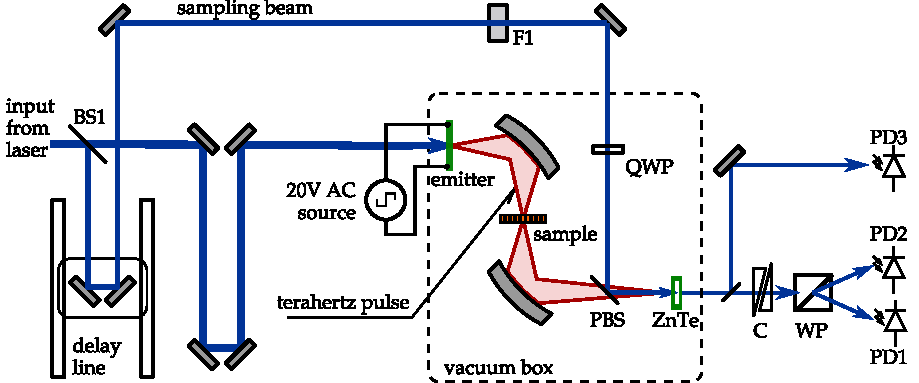
\includegraphics[width=\textwidth]{img/exp_THz_sampling.pdf}
\end{figure}

Before the laser pulse entered the vacuum chamber to induce the photoexcitation of the THz emitter, a small part of its energy was separated by a reflection from a beam splitter (BS1 in Fig. \ref{fg_exp}) into the \textit{sampling} branch. 

The pulse in the \textit{sampling} branch reflected from a pair of mirrors on a delay line, acquiring a precisely controlled relative delay against the terahertz pulse. Then it was attenuated at a filter (F1) and its polarisation was converted from linear to the circular one on a quarter-wave plate (QWP). The pellicle beamsplitter (PBS) directed the optical beam along the axis of the terahertz beam. 

We used the electrooptic sampling mentioned in the previous chapter: The electric field of the terahertz pulse induced a slight transient change in the permittivity tensor of the zinc telluride crystal (ZnTe). The much weaker and shorter optical pulse was modified by this change, acquiring diagonal ellipticity that could be fine tuned for zero signal with the Babinet compensator (C). The Wollaston prism (WP) was used to separate the two diagonal components of the resulting elliptic-polarized light. The difference between these two signals, if a small modulation is assumed, is proportional to the amplitude of the electric field. This allowed us to sample the electric field with a theoretical temporal resolution given by the duration of the optical pulse, but using a standard intensity detection using a pair of silicon diodes.   
%% TODO add references to other papers and theses from our group - one can not describe everything from Gouy shift to PKGraph ...

%}}}
\paragraph{Signal processing and acquisition}%{{{
To reduce the noise, synchronous detection with the \textit{Stanford SRS360} lock-in amplifier was used and the polarity of THz waveforms was modulated by the voltage at the TeraSED emitter. The difference signal at the two photodiodes, PD1 and PD2, was first fed to an analogue filter (with center frequency 91.3 kHz and 3 dB drop at $\pm$ 7 kHz), sampled by the lock-in amplifier and digitally normalized against the signal measured by the auxiliary photodiode PD3. The normalisation was necessary due to the fact that the difference signal is proportional not only to the terahertz field, but also to the laser intensity which may fluctuate over time. 

%The time constant of the lock-in acquisition was comparable to the time which was needed by the delay lines to introduce a picosecond delay. As a result, the speed of delay lines movement suppressed the high-frequency components of the detected signal. Attention must be paid at precise control of the delay line speed and software compensation of the artifacts.

The spectral response of both the emitter and electrooptic sampling substantially influenced the measured sample spectra. Moreover, the phase of the recorded waves was modulated too, as a beam passing through a focus acquires additional phase due to the Gouy shift \cite{kuvzel2010gouy}. Every transmission measurement was therefore normalized in frequency domain against a corresponding free-space reference, so that both the amplitude and phase artifacts cancelled out. 

%}}}

\subsection{Simultaneous reflectance and transmittance measurement}
\paragraph{Principle} %{{{
\label{srtm}
With rearrangement of optics, it would be possible to measure the \textit{reflectance spectrum}, similarly as the transmission was measured. However, due to the complexity of such a setup and its very high sensitivity to the sample displacement, we did not use a second sampling branch for detecting the reflected signal. Instead of using two sampling schemes, we recovered the amplitude and phase reflectance of the sample by stacking it between a pair of thick (3 and 6 mm) sapphire slabs \cite{nemec2012resonant}. Thanks to the relatively high refractive index of sapphire in the terahertz range along the optical axis, $N \approx$ 3.068, these slabs introduce several time-delayed pulse reflections, also called echoes, into the transmitted signal.
%\begin{figure} \caption{A broadband pulse passes through a single layer of microspheres randomly arranged between two sapphire slabs and is sampled by electrooptical detection.}  \centering 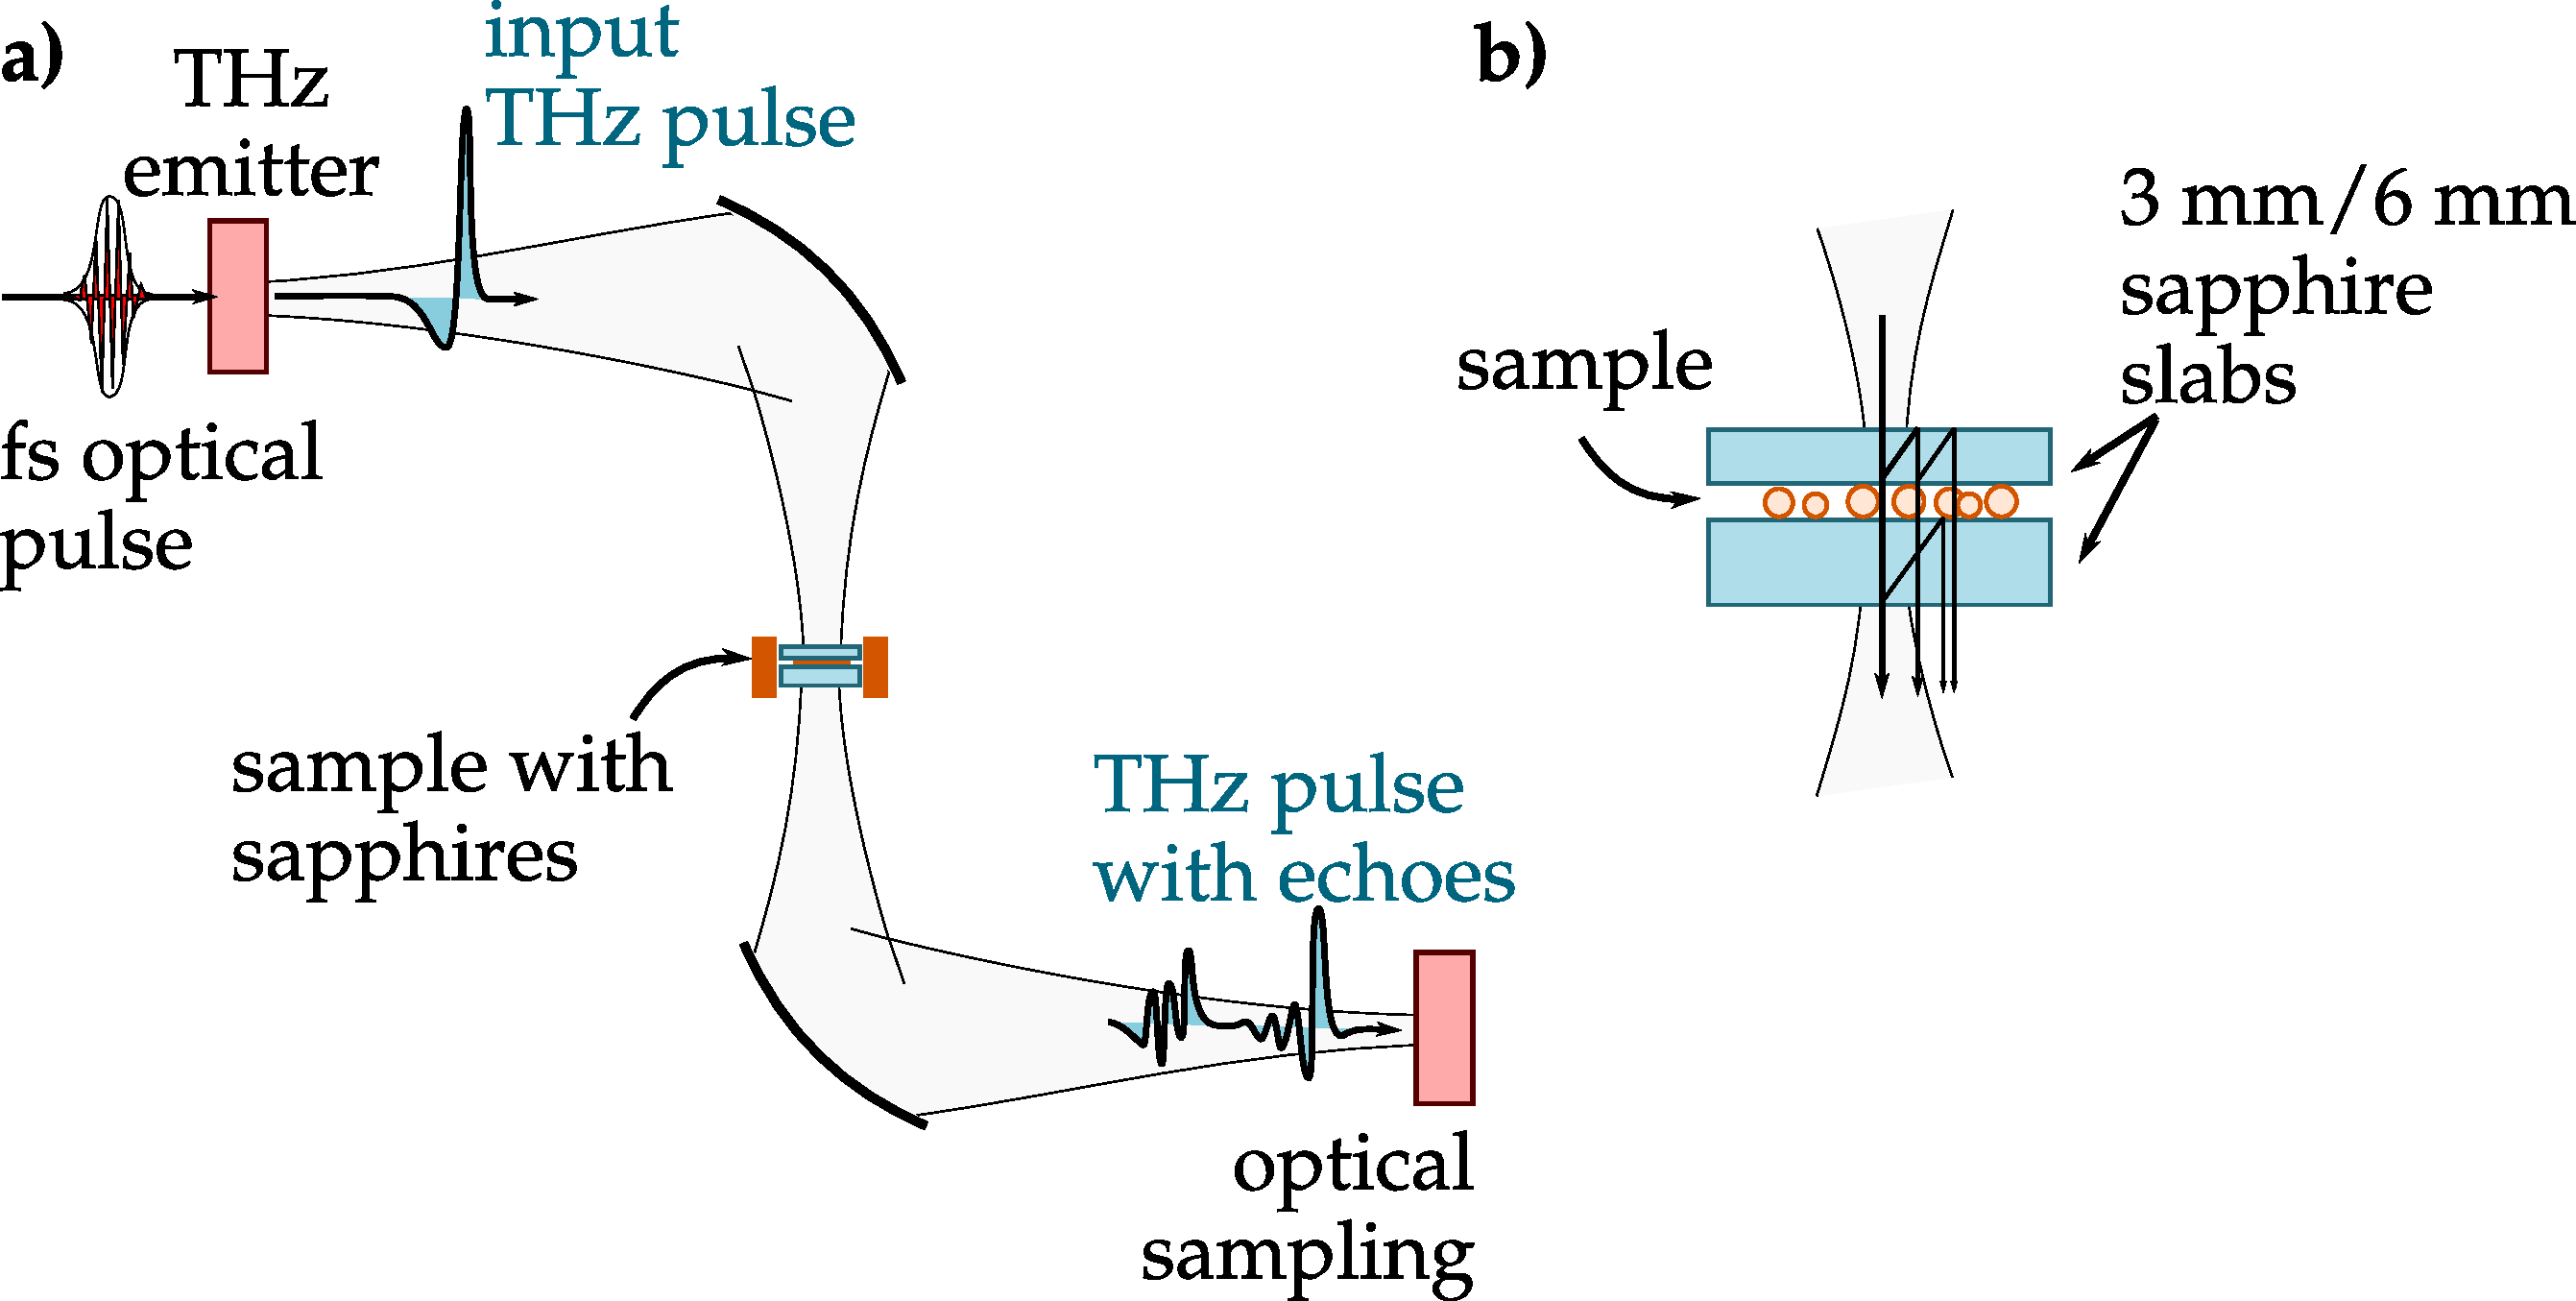
\includegraphics[width=12cm]{img/expe/sample_sapphires.pdf} \end{figure}			%% TODO no use for this figure?

If the beam divergence is neglected, each optical element can be characterised by its complex transfer function in the resulting spectrum. One needs to define three intrinsic transmittance functions: that for the beam passing through the volume of the thin sapphire $A(f)$, the one of the thick sapphire $B(f)$ and one through the thin sample $t_S(f)$; all of these are without the effect of reflection at interfaces. 

The reflection is described by two reflectance functions for the beam reflected on sapphire-air interface $r_{A}(f)$ and on the sapphire-sample interface $r_S(f)$.

By measuring the references of the thin and thick sapphires separately, the spectra of $A(f)$ and $B(f)$ as well as $r_{A}(f)$ can be established \cite{nemec2012resonant}. 

%defines the temporal separation between the main pulse and the first echo.  The reflectance and transmittance of the sample can be simply reconstructed using numerical deconvolution. The results of this method were, unfortunately, less than ideal. Among the reasons may be the possible asymmetry of the studied layer between the slabs, beam divergence and very low signal of both transmittance and particularly reflectance in the stop-bands of the sample.

To retrieve the characteristics of the sample, i.e. $t(f)$ and $r_S(f)$, the overall transmitted time-domain waveform of the sapphire-sample-sapphire structure has to be split into two parts that correspond to the direct pass, and the first echo arising from the pulse reflecting back and forth  in the thin sapphire.
The double propagation delay through 3 mm of the thinner sapphire is roughly 70 ps, which limits the spectral resolution to 14 GHz. All spectral features in the sample transmittance must be significantly broader than this value. Otherwise they could not be resolved, and even more importantly, their temporal ringdown would overlap in the time domain with the following echo and produce spurious results. Using a thicker sapphire could improve spectral resolution of this method, however it conflicts with the requirements of the terahertz beam fitting into the area of the sample \cite{nemec2009tunable} and of reducing the error caused by beam diffraction as noted in the following paragraph.

%}}}
\paragraph{Limitations of the scheme} %{{{
In the experiment, we observed substantial deviation  % TODO add some experimental data to {results} and  reference them here
from the numerically predicted results, which were moreover sensitive to subtle changes in the parameters. We propose  several independent explanations for the experimental errors:
\begin{enumerate}
\item{The geometrical beam divergence can not be fully compensated by the transfer functions of separate sapphire slabs, $A(f)$ and $B(f)$. 
The terahertz beam is relatively tightly focused, and the focus of the echoes is longitudinally displaced compared to the focus of the first pulse. 
The deconvolution algorithm can compensate for slight focus displacement by changing the amplitude  of different frequency components, or shifting them in phase. 

However, due to the hyperbolic shape of the gaussian beam, with its Rayleigh length $z_{R}$ being similar to the sapphire thickness\footnote{As an approximate example, for the main frequency component $f = 1.5$ THz with wavelength $\lambda = c / f \approx 200$~$\upmu$m, for $\vartheta \lesssim 0.15$ rad as an estimated divergence of the beam from its axis, the Rayleigh half-length of a gaussian beam would be $z_{R} = \frac{\lambda}{\pi \vartheta^{2}} \gtrsim 2.8$ mm, i.e. roughly the thickness of the thinner sapphire.}, the overall effect of two sapphires can not be linearly compensated from two separate measurements of each of them.} 
 \item{The possible asymmetry of the sample with regard to the beam axis can substantially bias the measured reflectivity. This happened during the characterisation of the dielectric spheres, when the sapphire distance was defined by a $\approx$60$\upmu$m teflon spacer. The nonuniform size of the resonators required us to attach them to one of the sapphire windows. While the spheres with the 60$\upmu$m diameter were placed symmetrically in the gap, the smaller spheres had an asymmetric position. Since the latter have higher resonance frequencies, the effect of asymmetry was probably also frequency dependent. } 
 \item{The sapphire slabs can influence the near field of resonances in some samples, c.f. Sect. \ref{par_nearfield}. This error should not be significant in transversally homogeneous samples (i.e. slabs), nor in samples that are made of dielectrics with much higher permittivity than that of sapphire. However for some samples, such as metallic resonators, the spectra are be completely changed in the vicinity of a dielectric (see its application on a fishnet sample in Fig. 4.19 in Ref. \cite{yahiaoui2011phd}). }
 \item{Finally, it follows from Eq. (\ref{eq_Neff}) that reliable reflection data can only be retrieved at frequencies where also the transmission amplitude is strong enough for the signal not to be dominated by noise. }
 \end{enumerate}
\label{srtm2}

%}}}

\section{Preparation of the titanium dioxide microspheres}
\paragraph{Fabrication through the spray-dry technique}%{{{
The collaborating laboratory of Dr. Patrick Mounaix in France %% Todo reference to Patrick's group somehow, and mention Oleg Mitrofanow (here, or later)
provided us with high-permittivity TiO$_{2}$ spheres with the sizes from 30 to 100 $\upmu$m, which were examined by the terahertz spectroscopy as dielectric resonators, and as possible constituents of a metamaterial with a negative effective permeability.
\begin{figure}[ht] \caption{Microphotograph of the TiO$_{2}$ spheres after preliminary sieving} \label{fg_microphoto} \centering 
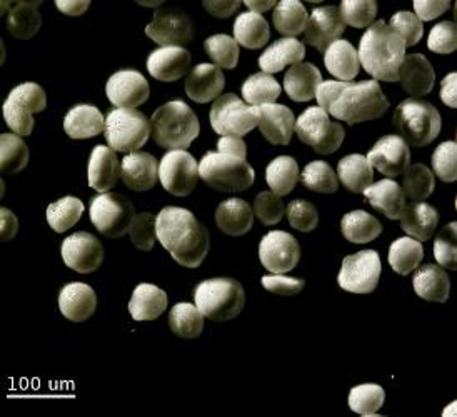
\includegraphics[height=5cm]{img/microscope_TiO2_particles.pdf}
\end{figure}

Compared to most metamaterial designs, the fabrication of the dielectric spheres can be extremely simplified by the \textit{spray-drying}\index{spray-drying technique} technique. In contrast with the expensive and time consuming \textit{top-down} processes such as laser cutting, litography or polishing, this is a typical \textit{bottom-up} process, where the particles are formed all within one procedure, though certain postprocessing is needed. 

As a first step, rutile (TiO$_{2}$) was ground to a sub-microscopic powder \cite[pp. 91-93]{yahiaoui2011phd}. A suspension of this powder in ethanol was sprayed into flame. It immediately formed spherical droplets, which dried up and sintered in the hot air. Rutile concentration in the suspension, feed rate and gas flow in the flame determined the average size of the sintered particles.

The resulting particles were annealed in a furnace to further solidify. The degree of recrystallization could be controlled  by the temperature of the furnace from 1200 to 1400 $^{\circ}$C from microscopic grains to few large crystalline domains in one microsphere. Note these temperatures used are still far below the melting temperature of rutile, which exceeds 1800 $^{\circ}$C.
Similar TiO$_{2}$ microspheres are also available commercially (e.g. from Brace, GmbH), and were likely made with a similar process.

The annealed spheres were further treated with the aim to break or eliminate clusters, by means of light milling with agathe mortar, which was separated afterwards by ultrasound bath cleaning in ethanol. Pre-sieving was performed on commercial sieves with 100, 53, 50, 40 and 38 $\upmu$m size of the square hole, though these nominal parameters of sieves should be in no way understood as hard limits for the particle sizes. The procedure of milling, cleaning and sieving was repeated 2-3 times, according personal communication with Dr. Patrick Mounaix and {Dr.} U-Chan Chung.

Only the low-temperature annealed samples were measured by the terahertz spectroscopy in this thesis. The fine-grained rutile was assumed to represent a nearly isotropic dielectric. We estimated the size of the constituent crystalline grains by grinding one microsphere and observing it under a polarizing microscope: unlike polycrystalline aggregates, small rutile monocrystals appear as coloured particles due to their inherent birefringence. In this way, the sizes of crystalline grains were assessed to be in the order of few micrometers or smaller.

%\textit{
%(\ldots) As the spheres have been sintered at high temperature, they have been separated from a platinum plate with a small soft paintbrush followed by a light milling with a agathe mortar. The goal was to separate the spheres that are welded to their neighbours due to the sintering step. All the spheres were treated in ultrasound bath using ethanol as a liquid phase. After natural drying, the sieving was performed. (\ldots) square (or rectangular) holes sieves were used. The meshes used were 106, 100, 53, 50, 40 and 38 micrometer. As a dry sieving step was performed, the particles were light milled again in order to try to break possible agglomerates which would not go through the mesh. This process was repeated 2-3 times and a final wet sieving with ethanol was performed in order to "wash" the spheres. No special measures were taken according to their shapes. (\ldots) } 
% TODO


%}}}
\paragraph{Theory of anisotropic sieves}%{{{
Triple sieving on commercial sieves, weaved from stainless steel wire, did not provide narrow enough size distribution, which is however essential for obtaining a narrow resonance peak of the sample. We therefore developed a more exact method for very fine sample sieving and characterisation. 

\begin{figure}[ht] \caption{Correspondence between the hole shape (above) and the set of ellipsoids that can pass through the hole (below), determined by their medium and minor axes. Somewhat surprisingly, the \textbf{(a)} square and \textbf{(b)} lozenge holes result in circular/elliptic set of passing particles, whereas the \textbf{(c)} circular and \textbf{(d)} elliptic holes result in the square/rectangular shape of such an region.\\
For clarity, some limiting-case examples of the ellipsoid projection and the equivalent position on the minor-major ellipse axis plot are drawn in blue, violet and red. } \label{fg_sieve_pass_notpass} \centering 
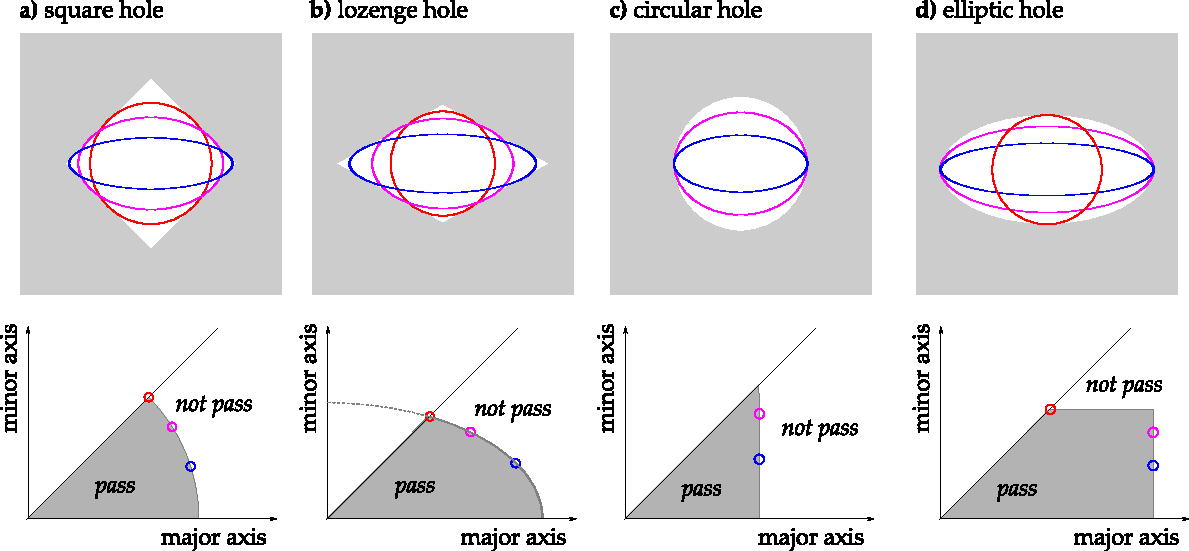
\includegraphics[width=\textwidth]{img/technology/sieve_pass_notpass.pdf}
\end{figure}
In the following, the dielectric particles are approximated by ellipsoids with three (generally different) half-axes $$\rho_a \leq \rho_b \leq \rho_c.$$ For the purpose of sieving, only the values of the shortest two half-axes, $\rho_a$ and $\rho_b$, decide whether the particle can pass through the sieve. The longest ellipsoid half-axis $\rho_c$ does not affect this, although it may influence the sieving speed. Therefore we can represent each three-dimensional particle with its projection on the smallest possible ellipse, which is described by its \textit{minor axis} $\equiv 2\rho_a$, and by its \textit{major axis} $\equiv 2\rho_b$ (which is, in fact, the \textit{medium axis} of the ellipsoid). For a given shape of a hole in a homogeneous flat sieve, it is easy to determine which values of minor and major ellipse axes allow a particle to pass through, and which not. For a square sieve such area in the parameter space forms a disk around the center of origin (Fig. \ref{fg_sieve_pass_notpass}a). It can be shown that when the sieve is diagonally stretched, forming a lozenge-shaped hole, the area of spheres allowed to pass transforms into an ellipse (Fig. \ref{fg_sieve_pass_notpass}b). When the hole shape is circular or elliptical, it is obvious that the area forms a part of a square or of a rectangle, respectively  (Fig. \ref{fg_sieve_pass_notpass}c,d).

The resonance frequency of a dielectric resonator depends on all three half-axes, $\rho_a \leq \rho_b \leq \rho_c$. In order to select a size fraction as narrow as possible, one has to use double sieving: the above sieve not allowing the fraction of particles too big, the bottom sieve removing the fraction of particles too small. This is where the anisotropic hole shapes become useful -- the bottom sieve can exclude also all oblong particles with the difference of $\rho_a \leq \rho_b$ too big. This effect is illustrated in Fig. \ref{fg_double_sieving}, which also presents a comparison between using more usual sieves with square/lozenge holes and the approach with a pair of sieves with micromachined square/elliptical holes. Obviously, the latter approach better discriminates between the \textit{shapes} of the ellipsoids. This advantage further gains on importance when the anisotropy of the sieve is low.

\begin{figure}[ht] \caption{Application of the effect from Fig. \ref{fg_sieve_pass_notpass} for separating a narrow fraction of ellipsoids between the sieves. Both combinations of \textbf{(a)} square-rectangular and \textbf{(b)} circular-elliptic sieves can be used, with the latter one promising better selectivity also in terms of the particle aspect ratio.} \label{fg_double_sieving} \centering 
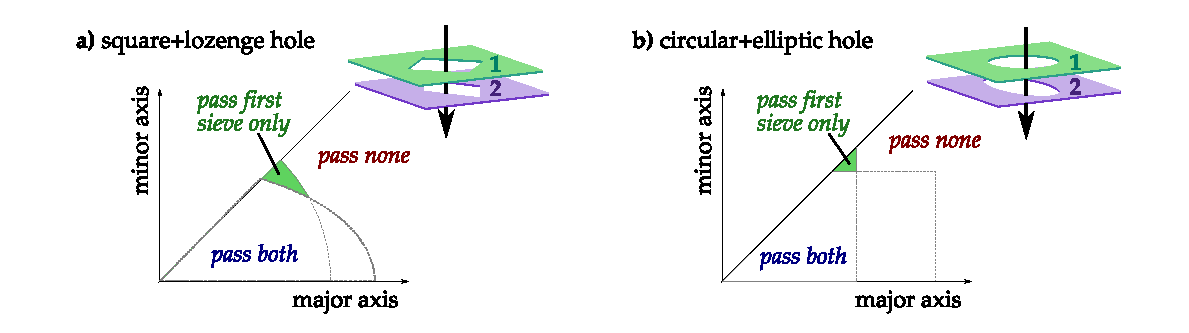
\includegraphics[width=\textwidth]{img/technology/sieve_double_sieving_fractions.pdf}
\end{figure}
It shall be noted that although we plotted a binary (pass/not pass) function in Figs. \ref{fg_sieve_pass_notpass} and \ref{fg_double_sieving}, the sieving speed continuously drops when the particle dimensions approach those of the sieve holes. 
%For any finite sieving time, this obviously affects the statistics of particles passing the sieve, favoring the average size to be lower for short sieving times.
However, this particular fraction of particles is exactly what one is interested in during the high-accuracy sieving. The process must therefore be run for a long enough time, of the order of days, and with as high a sieving speed as possible.
%}}}
\paragraph{First sieving apparatus}%{{{
%Finally, they were carefully sieved in many iterations, to select a size fraction as narrow as possible.
Employing the idea of anisotropic sieves from Fig. \ref{fg_double_sieving}a, the author assembled a first prototype based on nylon sieves, as depicted in Fig. \ref{fg_sieving1}. Two glass containers, 6 mm high and 11 mm in diameter, were cut on a lathe from a glass tube. On their bottom, the sieves were glued and carefully clipped. The side of the sieve holes was 60$\pm$5 $\upmu$m. 

The mesh was woven of nylon threads, so the bottom sieve could easily be stretched by ca. 20-25 \% in the diagonal direction.  The above sieve was kept isotropic. 

This  property however prove to be also detrimental for precise sieving, as the threads easily bent aside under only a small force, thus allowing oversized particles either to pass or to get stuck permanently and to block the sieve within few minutes. To help resolving the latter problem, two additional narrow glass rings were cut from the glass tube, supporting much coarser sieves with 150 $\upmu$m pitch glued on the bottom, to allow little spherical springs bounce beneath the sieves and to loosen the particles that got stuck in the holes. For the same purpose, 2mm plastic balls were added to the microsphere samples.  

A cover on top prevented the particles to jump out of the above container. The whole stack was carefully lowered into a test tube with a greater diameter, and vibrated by a tiny electric motor glued on the bottom.

\begin{figure} \caption{\textbf{(a)} Photograph and \textbf{(b)} scheme of the first sieving apparatus based on square-lozenge sieve pair, with a schematic out-of-scale illustration of its operation for an input of four different microspheres \textbf{(c)}}  \centering 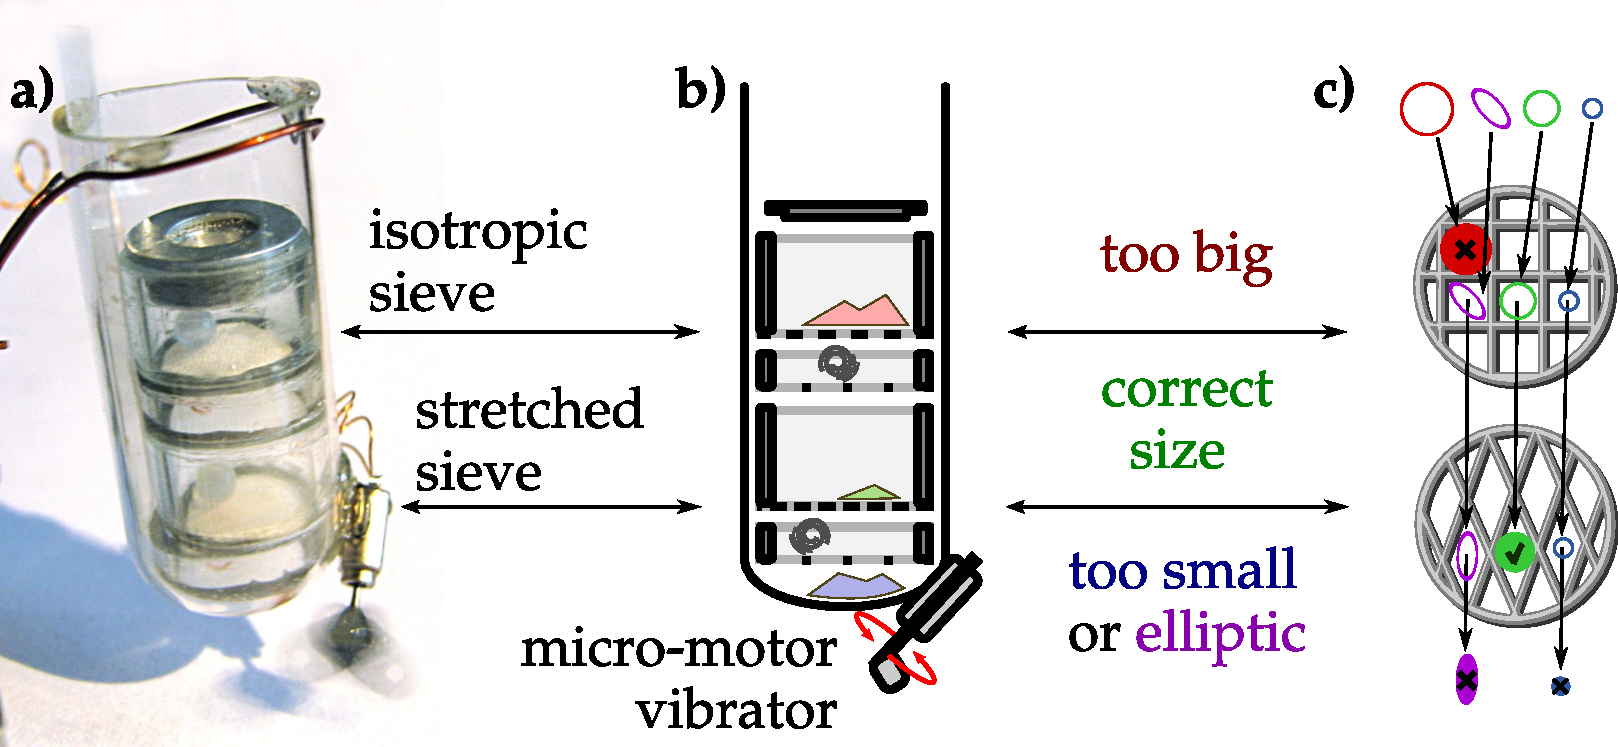
\includegraphics[width=12cm]{img/expe/sieving1.pdf} \label{fg_sieving1} \end{figure} 

%}}}
\paragraph{Second sieving apparatus}%{{{
\begin{figure}[ht] \caption{\textbf{(a)} A sketch of the acoustic sieving device, and \textbf{(b)} a photograph thereof} \label{fg_sieving2} \centering 
	\begin{overpic}[height=.4\textwidth]{img/technology/sieve2_sieving_scheme.pdf}  \put(-10,93) {\textbf{(a)}} \end{overpic}
	\begin{overpic}[height=.4\textwidth]{img/technology/sieving_m.pdf}              \put(1,85) {\textbf{(b)}} \end{overpic}
\end{figure}
The partially promising results and, more importantly, obvious deficiencies of the previous apparatus motivated the construction of a second one depicted in Fig. \ref{fg_sieving2}.
Different from any other sieving apparatus known to the author, this one made use of vertical acoustic waves for the movement of particles. It consisted of two coaxial glass tubes: The inner tube, with outer diameter of 13 mm, had a round metallic sieve glued to its bottom, and on its upper end it was covered by a small acoustic transducer. The outer tube (90 mm long, outer diameter 26 mm) surrounded the inner one and had a round bottom, where the particles were collected. 

The gaskets ensured that the whole apparatus was tightly closed, preventing both sieved particles and the sound from escaping. The brass ring with the transducer was fixed to a massive aluminum stand, and the rest of the structure was held by two accessible screws that allowed easy disassembling. 

The key advantages of this novel approach are the following:
\begin{enumerate}
 \item{The speed of sieving is expected to grow with the frequency at which the particles hit the sieve. The acoustic frequency of 1 kHz is roughly two orders of magnitude higher than in usual commercially available devices. Moreover, the spheres are  continuously stirred, so it is ensured that a layer of over-sized particles does not occupy the sieve.} 
 \item{The upward air pressure pulls out particles that got stuck in the sieve in every period of acoustic vibration. This resolves the major issue of clogging inherent for the previous prototype.} 
 \item{Avoiding macroscopic vibrating parts, except the membrane of a small acoustic transducer, allows the device to operate over multiple days with reduced risk of mechanical failure.}
 \end{enumerate}
The outer tube acted as an acoustic resonator, greatly enhancing the effect of the sound when tuned to resonance around 750-900 Hz. These frequencies obviously correspond to the fundamental acoustic resonance, as the corresponding quarter-wavelength is close to the 10 cm length of the outer tube.  The electrical input power of the sine wave feeding the device was in the order of 1 W.

%}}}
\paragraph{Sieving challenges}%{{{
A practical deficiency of this setup was that the upper opening of the transducer radiated relatively intense sound during operation. We resolved this potential issue by covering the whole apparatus by a robust glass bell jar.

With the acoustic power and frequency correctly adjusted, the particles formed a cloud 5--10 mm high. One difficulty arose from that the small particles tend to attach to the surface of glass or metal, probably due to electrostatic charges on their surface. While at an average particle radius $\rho = 50$ $\upmu$m this effect was rather marginal and transient, it took only few seconds of sieving for $\rho = 20$ $\upmu$m particles to immobilize permanently on any surface. It has however proven efficient to tap the upper brass ring, as the mechanical shock released most spheres and renewed the sieving process. To ensure unattended sieving for a timespan in order of days, we added a little motorized hammer with a timing circuit (Fig. \ref{fg_sieving2}a).

The amount of particles in one batch was limited to ca. 10--20 mm$^{3}$, otherwise the sieve would be covered with a layer too thick, which could not be efficiently lifted by the acoustic pressure.
This problem could however be slightly mitigated by tilting the apparatus. With a tilt of 5--10 degrees, the bulk of particles then accumulated near one side, leaving most of the sieve surface free for sieving the moving particles. Given the small amount of particles required for the terahertz spectroscopy measurements, it is however advisable to sort a batch in order of 1--3 mm$^{3}$.

%}}}
\section{Optical determination of microparticle statistics}
\paragraph{Image preparation} %{{{
An accurate characterisation of the particle statistics was necessary not only to assess the efficacy of sieving, but also to explain  on a quantitative basis possible differences between the measured terahertz spectra and the computed ones. To obtain reliable statistics, thousands of particles needed to be evaluated, repeatedly for every sample. This, along with the small dimensions of particles, indicated that the most viable way to do so would be the optical microphotography with computer image processing automatically resolving each particle.

Computer \textit{granulometry}\index{granulometry}, identification and measurement of photographed particles from a digital image,
is a well-established technique. It is implemented in several advanced image processing programs, of which \textit{ImageJ} was selected \cite{abramoff2004image} since it is free of charge and allows its use for large batches of images through the use of macros. 

The transmission microphotographs were acquired either with the lowest magnification on a laboratory microscope, or with a portable microscopic digital camera on its highest magnification, yielding similar results.

The first processing step, applied at the somewhat blurred photographs, as shown in Fig. \ref{fg_sievingstats}a, was to establish the intermediate brightness level between the image's bright and dark areas, and apply a threshold so that the image was a binary function. Then the \textit{ImageJ}'s \textit{watershed} algorithm was applied to relatively reliably resolve two or more touching particles, and a particle outline was found. An example is depicted as cyan lines in Fig. \ref{fg_sievingstats}b. Finally, the particle outlines were approximated by best matching ellipses, and the major and minor axes of the ellipse were added into the statistics. 
\begin{figure}[ht] \caption{\textbf{(a)} A small section of a microphotograph of a pre-sieved sample before applying the described double-sieve method, \textbf{(b)} the corresponding identification of particles in ImageJ} \label{fg_sievingstats} \centering 
	\begin{overpic}[height=.30\textwidth]{img/technology/imagej_photo.pdf} \put(-9,72) {\textbf{(a)}} \end{overpic}\quad\quad
	\begin{overpic}[height=.30\textwidth]{img/technology/imagej_found.pdf} \put(-9,72) {\textbf{(b)}} \end{overpic}\quad\quad
\end{figure}
We complemented the \textit{ImageJ} macro with a Python script enabling us to process multiple photographs in a batch, and to plot the resulting histograms of the ellipse axes distribution. The script has also been published online \cite{dominec2014_imagej}. The scale for each batch of images had to be determined from a separate photograph of a ruler.

%}}}
\paragraph{Imprecision of the method} %{{{
An intrinsic deficiency of this method is that it was not possible to resolve the third dimension of particles. 
It can be however estimated that when % TiO$_{2}$ 
ellipsoidal particles were randomly sprinkled on the glass, they would lie mostly on their flat side -- i.e. their orientation would enable to measure the \textit{medium} $\rho_b$ and \textit{major} axes $\rho_c$ of the ellipsoid. This is in contrast with the process of sieving, as described above, where the particles were sorted according to their and \textit{minor} $\rho_a$ and \textit{medium} $\rho_b$ axes. 

This source of error is probably similarly important as another one, arising from rough shapes of the particles which could not always be well approximated by an ellipsoid. 
%\todo{add the previous and resulting statistics? the THz spectra should better go to the Results }
%}}}

\section{Laser cutting}
\paragraph{Fabrication of dielectric bars}%{{{
Dielectric or metallic structures can be made by cutting a thin polished slab of the given material. Electromagnetic waves with a frequency of  1 THz have a free-space wavelength of 0.3 mm. Periodic structures designed to operate in this range have their unit cells of a similar size or less, and their finest features are usually in the order of 10-20 $\upmu$m. 

The sample already shown in Fig. \ref{fg_STO_bar_rt} consisted of bars from strontium titanate (SrTiO$_{3}$) with a rectangular cross-section (see Fig. \ref{fg_STO_bar_geom}), where a structure with 10--30 $\upmu$m lateral bar dimensions was engraved into a thin slab of the dielectric of a similar thickness \cite{yahiaoui2011tunable}.

If the slab consists of a monocrystal or a ceramic, it is usually extremely brittle and also sensitive to breaking due to thermal stresses. Femtosecond laser cutting (or, micro-machining) is suitable for such a task because it delivers the energy so fast that most of the heated material evaporates before the heat can diffuse into the rest of the structure. 
The strontium titanate bars were fabricated by the \textit{Alphanov} facility in France.

%}}}
\paragraph{Fabrication of sieves and fishnets}%{{{
Femtosecond cutting of metallic sheets into two-dimensional meshes is relatively easy,   
compared to the dielectrics, 
and was implemented in our laboratory. To achieve the required precision, we used 20 or 30 $\upmu$m thick high-quality stainless steel foils. 

The femtosecond laser used was different from that serving as the femtosecond source for terahertz spectroscopy (Sect. \ref{sect_tdts}). A largely sufficient power was provided by the \textit{Spectra Physics Spitfire Ace} multipass titanium-sapphire amplifier, with 1 mJ of energy per impulse, duration of $\sim$50 fs, and 5 kHz repetition rate. Its output beam had to be attenuated to obtain finer cut at the expense of a slightly slower speed. The mechanical part consisted of two crossed \textit{Owis} stepper-motor controlled linear stages, and a fast mechanical shutter allowed us to control the beam with a sufficient resolution of ca. 100 ms. 
\begin{figure}[ht] \caption{\textbf{(a)} Laser cutting the steel foil with a moving holder for four samples, metal vapour ventilation, and the focusing lens. Bright plasma spot is visible at the focus. \textbf{(b)} The resulting sieves made from 30 $\mu$m stainless steel foil with 10 mm overall diameter.} \label{fg_microfab} \centering 
	\begin{overpic}[height=.35\textwidth]{img/technology/sieve2_drilling_m.pdf} \put(-8,82) {\textbf{(a)}} \end{overpic}\quad\quad
	\begin{overpic}[height=.35\textwidth]{img/technology/steel_sieve_on_paper.pdf} \put(-8,80) {\textbf{(b)}} \end{overpic}
\end{figure}

The 3 mm wide beam was focused by a lens with a focal length of 10 mm or 50 mm (Fig. \ref{fg_microfab}a). The tighter focusing lead to a better resolution, but had stricter requirements for accurate focusing of the beam. To facilitate the task of optimal focusing, we devised a focusing-collimating setup which used the fact that  the  steel foil reflected the light like from a point source only when it was exactly in the lens focus. Then the reflected light would be collimated again by the very same lens into a beam returning to the laser. 
%the reflection would not be collimated if the reflection occurred in front of the focal plane or behind it. 
A part of the reflected beam energy was reflected sideways by a skewed glass in front of the lens, so that one could finely align the lens seeking for the smallest spot diameter on a distant screen.

A compact stepper-motor controller of a custom design \cite{dominec2015_triostepper} facilitated to automate the sample movement by means of computer control operated by a Python script. The sequences of shutter opening, sample movement and shutter closing could be assembled into a program for fabrication of a whole mesh sample of ca. 10 mm diameter, which took about 30 minutes to finish. Multiple different meshes with different parameters could be cut out from one steel foil in a batch, without user interaction.

%}}}
\paragraph{Laser cutting issues}%{{{
The metal evaporated during the laser cutting immediately oxidises in the air. Although in total only few milligrams of the stainless steel foil were removed, the microscopic particles would pose a risk of damaging optical components. We built a miniature ventilation and filtering system out of a tube filled with cotton wool and fine synthetic fibers. After few meshes were cut, the cotton changed its colour from white to pale brown, indicating that at least a part of the particles were filtered out.

A greater challenge arose from thermal expansion of the foil. In order to fully utilise the valuable laser beam time, one would wish to set the cutting speed as high as possible. However, the speed of cutting was rather limited by the speed of stepper motors. The heat remaining in the steel foild was high enough to cause its thermal expansion and bending out of the plane of its holder. Even though the resulting displacement was less than 1 mm, the sheet moved significantly out of the beam focus. We assume this was the reason for slight variations between the hole sizes in Fig. \ref{fg_fishnet28_photo}. The effect would be diminished through slower cutting speed or by gluing the foil to a sacrificed rigid substrate.

Cutting the foil into free-standing wire array was however not successful since the resulting thin wires bent out of their original plane due to the thermal expansion. Their spacing was so uneven that no usable sample of wires was made.

%}}}
\paragraph{Difference between sieves and fishnets}%{{{
The meshes were made for two purposes -- either as sieves used in the second sieving apparatus described above, or as metamaterial samples known as \textit{fishnets}\index{metamaterial!fishnet!fabrication}, which are predicted to exhibit a negative index of refraction (see Sect. \ref{section_fishnet}). The difference between these applications is subtle; the meshes intended as sieves would surely exhibit a resonance in the terahertz range. 

The optimum  size range for the titanium dioxide spheres resonating around 1 THz is around 30--60 $\upmu$m, which determined the hole diameter of sieves. To maintain mechanical robustness, the periodicity in sieves was kept much larger than the hole diameter, usually 300$\times$300 $\upmu$m, and the thickness was chosen as 20 or 30 $\upmu$m.
The fishnets had the same periodicity as sieves, and the hole dimensions were chosen between 150 and 280 $\upmu$m. 
For cleaner cutting, a thinner stainless foil was used, with a thickness of 5 $\upmu$m.

% TODO
%To achieve the required precision of sieving, we fabricated the sieves by femtosecond laser drilling of 20--30 $\upmu$m thick stainless steel steel foil
%These sieves then were employed in a device that subjected the microsphere sample to acoustic vibrations, improving the speed of the demanding sieving process to acceptable level

%}}}


\chapter{Results}

%% TODO remaining topics to be added or checked: 
% 

%%	* PhCs with metallic/metamaterial inclusios, [Monsoriu, Lina Shi and friends]
	%thin wires [8], [28], Swiss rolls [9], SRRs [9], electric SRRs (eSRRs) [29], [30], pairs of rods [10], [12], [31], pair of crosses [32], fishnets [17], [33]”


\label{chapter_results}
\section{Dielectric slab} \label{section_Dielectric slab}
\paragraph{Dispersion curves of a one-dimensional photonic crystal}
\begin{figure}[h] \caption{Dispersion curves \textbf{(a)} in free space with virtual periodicity $a$, \textbf{(b)} in dielectric layers with permittivity $\varepsilon = 12$ and 15 \% fill fraction. \\

Side plots show the electric field in $2\times 2$ unit cells, with dielectric outlined by thin black lines. The electric field was chosen to be polarized along the $x$-axis and is plotted as a color map (white corresponding to zero).} \label{fg_1dbd} \centering 
	\begin{overpic}[width=.48\textwidth]{img/Slab_eps001_PWEM.pdf}  \put(1,96) {\textbf{(a)}} \end{overpic}
	\begin{overpic}[width=.48\textwidth]{img/Slab_eps012_d15.pdf}   \put(1,96) {\textbf{(b)}} \end{overpic}
\end{figure}
\begin{figure}[t] \caption{Amplitude of \textbf{(a)} reflectance, \textbf{(b)} transmittance and \textbf{(c)} effective index of refraction $\Neff$ (real part solid, imaginary part dashed) for the dielectric slab of 15\% fill fraction in a 300 $\upmu$m unit cell, and varied permittivity of the dielectric $\epsrl \in \{4,12,20\}$} \label{fg_Slab_fillfraction015_epsilon_comparison} \centering \vspace{-3mm}
\begin{tabular}{r}
\begin{overpic}[width=0.95\textwidth]{img-meep/Slab_fillfraction015_epsilon_comparison_r.pdf} \put (-1,27) {\textbf{(a)}} \end{overpic}\vspace{-0.055\textwidth}\\
\begin{overpic}[width=0.95\textwidth]{img-meep/Slab_fillfraction015_epsilon_comparison_t.pdf} \put (-1,27) {\textbf{(b)}} \end{overpic}\vspace{-0.055\textwidth}\\
\begin{overpic}[width=0.96\textwidth]{img-meep/Slab_fillfraction015_epsilon_comparison_n.pdf} \put (-1,37) {\textbf{(c)}} \end{overpic}\vspace{-0.\textwidth}\\
\end{tabular}
\end{figure}
The one-dimensional photonic crystal (1-D PhC) has been investigated thoroughly in the previous century and found its major application in dielectric mirrors. It is the simplest representative of periodic structures, since  it exhibits only a subset of different phenomena that can be observed in other periodic structures. This is due to its continuous translational symmetry in the transverse direction that excludes all phenomena with a lower symmetry. 

Most importantly, no \textit{individual resonances} can occur in 1-D PhC; all interaction with the wave happens through partial reflection of the electromagnetic wave on the interfaces of the layers. The only type of the band gap observed is of the Bragg type.

Dispersion curves for two examples of one-dimensional photonic crystals were computed using PWEM and are shown in Fig. \ref{fg_1dbd}. 
Its left panel shows the folded dispersion curves for a plane wave propagating in vacuum on which we imposed virtual periodicity. To save space, the dispersion curves were plotted as \textit{folded}, but one can easily imagine how the curve unfolds into a linear dispersion of vacuum, known as the \textit{light line}. No scattering occurs for homogeneous vacuum, thus for any frequency $f$ exists a real wavenumber $k$ corresponding to a propagating wave and there are no band gaps of finite width. 

The right panel, Fig. \ref{fg_1dbd}b, is obtained by introducing periodic layers of dielectric with permittivity 12\% and 15\% filling fraction. The dielectric is outlined by thin black lines. Band gaps of nonzero width corespond to frequency ranges where the wave can not propagate through the structure. %TODO The first photonic band gap starts at the frequency, TODO at which exactly half wavelength matches the cell spacing, i.e. when $2\pi / K= a/2$ as is depicted in the subplot \textit{X1} of Fig. \ref{fg_1dbd}b. The next band starts at the same wavenumber $K$, but the wave now has higher frequency because in the subplot \textit{X2} of Fig. \ref{fg_1dbd}b it is shifted by half its period so that it maximizes the electric field energy that is localized in the areas of lower permittivity. Higher Bragg band gaps are formed by the same mechanism.

\paragraph{Characteristics of Bragg-type band gaps}
The lower and upper edge of the photonic bands are located the high-symmetry points of the Brillouin zone, such as $\mathbf{\Gamma}$ or $\mathbf{X}$, which are equivalent to the wavenumber $K=m\pi/a$ for $m\in\mathbb{Z}$ in the one-dimensional case discussed. Whenever $K$ is in one of these points, the electric and magnetic fields are periodic in space, and can be easily visualized. The side plots of \ref{fg_1dbd} show the shapes of the electric field $E_x$ in the $(y,z)$ plane at respective frequencies of the band edges. To stress the fact that the field is periodic even in the $\mathbf{X}$ point, each of the side plots spans over 2$\times$2 unit cells. 

An important characteristic of each field pattern is the set of all points where the field amplitude remains zero over the evolution of time. Such sets will be denoted as \textit{nodal planes}, or also, more accurately, \textit{nodal surfaces}.

From all pairs of field plots that are connected by a photonic band (i.e. X2-$\Gamma2$, $\Gamma3$-X3 etc.), it can be deduced that one nodal plane dividing the unit cell in perpendicular orientation to the wave vector is always added when the frequency increases from the lower band edge to the upper one. This rule is more general and is satisfied by other structures, too. 

Typical for all Bragg band gaps (i.e. X1-X2, $\Gamma2$-$\Gamma3$, etc. in \ref{fg_1dbd}) is that between the lower and upper edges of each band gap, the phase increase across an unit cell does not change and thus $K$ remains constant, as does the number of the nodal planes. The field does change between these points, however, and the change is in the location of the \textit{nodal planes} such that the upper band-gap edge concentrates the field energy in mostly lower-permittivity regions. 

\paragraph{Bragg and Fabry-Pérot resonances}
The \textit{Bragg condition} for the formation of a band gap in a periodic structure is that an integer number of half waves fits into the unit cell; i.e. that the phase difference $\phi_{1+2}$ of the wave along the unit cell is 
\begin{equation} \phi_{1+2} = d_1 n_1 \frac{\omega}{c} + d_2 n_2 \frac{\omega}{c} = \pi m, \text{ where } m\in \mathbb{Z}. \label{eq_braggcond}\end{equation}
where $d_{1,2}$ are the thicknesses and $n_{1,2}$ are the refractive indices of the two layers.

\begin{figure}[t] \caption{\textbf{(a)} Reflectivity and \textbf{(b)} the imaginary part of the retrieved refractive index for a 1-D PhC, with filling fraction of 15\% in a 300 $\upmu$m unit cell, as a function of frequency and dielectric permittivity. On the right panel, the Fabry-Pérot condition from Eq. (\ref{eq_fpcond}) are marked by a thin dash-dotted line.} \label{fg_slab_eps_scan} \centering 
\begin{overpic}[width=0.48\textwidth]{img-meep/Slab_fillfraction015_epsilon_scan_r.pdf}\put (1,80) {\textbf{(a)}}\end{overpic}
%Slab_fillfraction015_epsilon_scan_r.pdf
%Slab_fillfraction015_epsilon_scan_t.pdf
\begin{overpic}[width=0.48\textwidth]{img-meep/Slab_fillfraction015_epsilon_scan_ni.pdf}\put (1,80) {\textbf{(b)}}\end{overpic}  % TODO rm voids
%Slab_epsilon4_fillfraction_scan_r.pdf
%Slab_epsilon4_fillfraction_scan_t.pdf
\end{figure}

\begin{figure}[t] \caption{\textbf{(a)} Reflectivity and \textbf{(b)} the imaginary part of the retrieved refractive index for a 1-D PhC, with dielectric permittivity of 4, as a function of frequency and filling fraction in a 300 $\upmu$m unit cell} \label{fg_slab_ff_scan} \centering 
\begin{overpic}[width=0.48\textwidth]{img-meep/Slab_epsilon4_fillfraction_scan_r.pdf}\put (-1,80) {\textbf{(a)}}\end{overpic} % TODO  lower number of contours
%Slab_fillfraction015_epsilon_scan_r.pdf
%Slab_fillfraction015_epsilon_scan_t.pdf
\begin{overpic}[width=0.48\textwidth]{img-meep/Slab_epsilon4_fillfraction_scan_ni.pdf}\put (-1,80) {\textbf{(b)}}\end{overpic} % TODO rm voids
%Slab_epsilon4_fillfraction_scan_r.pdf
%Slab_epsilon4_fillfraction_scan_t.pdf
\end{figure}
%\clearpage

The width of the band gap grows with the amplitude of the wave scattered from the unit cell. This amplitude however also depends on frequency and, in the case of a lossless dielectric slab, it vanishes whenever an integer number of the half-waves fits into either of the dielectric layers. For comparison with Eq. (\ref{eq_braggcond}), this condition is
\begin{equation} \phi_{1} = d_1 n_1 \frac{\omega}{c} = \pi m \text{\quad or \quad} \phi_{2} = d_2 n_2 \frac{\omega}{c} = \pi m, \text{ where } m\in \mathbb{Z}. \label{eq_fpcond}\end{equation}
Note that unlike the Bragg resonance, this effect can be observed even in a single isolated unit cell; in fact it is the well known \textit{Fabry-Pérot resonance}. 

The vicinity of a Fabry-Pérot resonance influences the position and width the neighbouring band gap, which can be found for different dielectric permittivity of the slab $\epsrl\in\{4,12,20\}$ in Fig. \ref{fg_Slab_fillfraction015_epsilon_comparison}.

A special case can occur when the conditions for both Bragg and Fabry-Pérot resonances are fulfilled simultaneously: a \textit{zero-width band gap} is obtained and two photonic bands are adjacent to each other in the same way as they were in vacuum (c. f. Fig. \ref{fg_1dbd}a). An example of a structure that exhibits multiple zero-width band gaps is the 1-D PhC with equal optical thickness of both slabs ($d_1 n_1 = d_2 n_2$), but multiple such points can be found when the dielectric permittivity or the dielectric filling fraction is changed, as depicted in Figs. \ref{fg_slab_eps_scan} and \ref{fg_slab_ff_scan}, respectively. These plots are also the simplest examples of the interplay between the individual resonance contained in the dielectric structure and the overall band-gap structure, a topic that will be discussed later in more detail.

\paragraph{Local effective parameters of a 1-D PhC}
Employing the \textit{s-parameter} method based on FDTD simulation, as described in Chapter \ref{chapter_sparam}, one can obtain the scattering parameters (i.e. complex reflectance and transmittance) of a finite layer of the periodic structure, and eventually retrieve its local effective parameters: the index of refraction $\Neff(f)$, impedance $\Zeff(f)$, permittivity $\eeff(f)$ and permeability $\meff$. The first one is plotted in Fig. \ref{fg_Slab_fillfraction015_epsilon_comparison}c, allowing to clearly identify the Bragg band gaps as regions where $\Neff'$ follows one of the Brillouin zone boundaries and $\Neff'' < 0$.

The question is to what extent the three remaining local parameters, $\Zeff$, $\eeff$ and $\meff$, have any physical meaning. As a generally accepted approach, they will be considered meaningful only for the long wavelength limit, i.e. $K$ close to the $\mathbb{\Gamma}$ where the effects of the spatial dispersion should be negligible. According to Fig. \ref{fg_Slab_fillfraction015_epsilon_comparison}c, this is for frequencies up to 100 or 200 GHz only. At any higher frequency, the retrieved wavenumber $K$ approaches the Brillouin zone boundary, marked by the dash-dotted line, and grows further.


In the low frequency limit of 1-D PhC, it was always observed that
\begin{enumerate}
\item{$\Zeff \approx 1/\Neff$, thus the effective permeability is $\meff = \sqrt{\Neff\Zeff} \approx 1$.} 
\item{The effective permittivity $\eeff$ is the weighted average of the constituent media, which determines the low-frequency limit for the refractive index:
	\begin{equation} \left.\Neff\right|_{K\ll 2\pi/a} =\left. \sqrt{\eeff}\right|_{K\ll 2\pi/a} \approx \sqrt{\frac{d_1 n_1^{2} + d_2 n_2^{2}}{d_1+d_2}} \label{eq_phc_eeff}\end{equation}
	}
\end{enumerate}
Notice in Fig. \ref{fg_Slab_fillfraction015_epsilon_comparison}c that $\Neff$ at higher frequencies converges towards its asymptotic value $\left.\Neff\right|_{K\rightarrow +\infty}$, which differs from the value obtained by Eq. (\ref{eq_phc_eeff}):
\begin{equation} \left.\Neff\right|_{K\rightarrow +\infty} \approx \frac{d_1 n_1 + d_2 n_2}{d_1+d_2} \label{eq_phc_neff}\end{equation}
The difference comes from that in the low-frequency limit, the electromagnetic energy concentration is higher in the areas of higher permittivity, whereas in the high-frequency limit it appears to be distributed evenly.
Note that with the correct branch retrieval procedure, the index of refraction never drops with frequency except for the photonic band gaps. Negative derivative of $\Neff(f)$ would otherwise imply that the group velocity would be higher than the phase velocity \cite{mikki2009electromagnetic}, which was never observed in 1-D PhC.

% TODO \paragraph{Transmission through a finite number of unit cells}
% illustrate the band-gap formation \cite{laktionov2008}
% (todo) find python script ----> compare TMM and FDTD for metallic slabs
% note the ripples inside the band-gap (for more cells)
% and note that the NRW effective parameters do not change; the method is exact here due to absence of evanescent fields, whose detrimental effect was described in -todo-
% finite planar structure with defect mode \cite{skoromets2013}
%\begin{figure} \caption{1red.pdf}  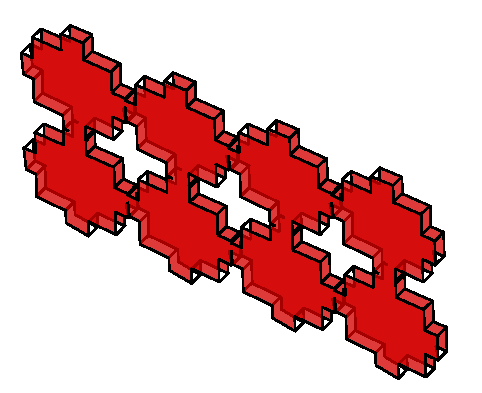
\includegraphics[width=3cm]{img/multilay_1red.pdf}
               %\caption{2gn.pdf}   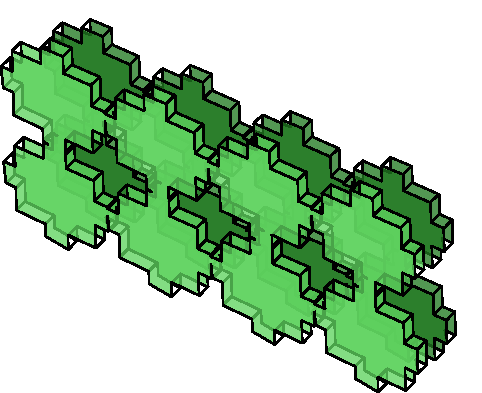
\includegraphics[width=3cm]{img/multilay_2gn.pdf}
               %\caption{3bu.pdf}   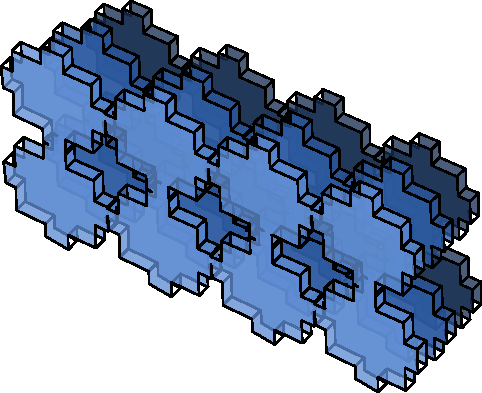
\includegraphics[width=3cm]{img/multilay_3bu.pdf}
               %\caption{3grey.pdf} 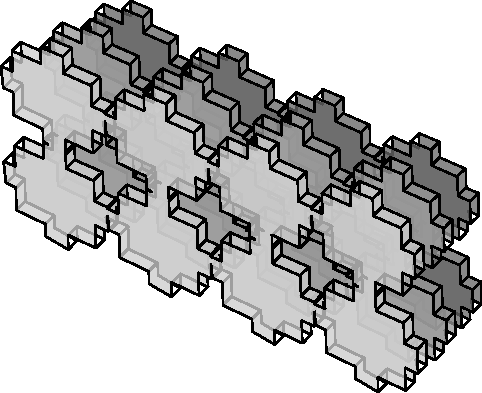
\includegraphics[width=3cm]{img/multilay_3grey.pdf}
               %\caption{4vio.pdf}  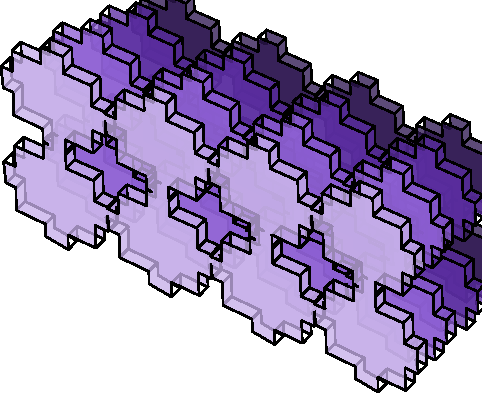
\includegraphics[width=3cm]{img/multilay_4vio.pdf} \end{figure} \clearpage

\clearpage

%====================================================================================================
\section{Wire medium} \label{chap_wiremedium} % references to -> %{{{ \label{section_
\paragraph{High-frequency behaviour}
The structure formed of a regular square lattice of conductive wires exhibits more interesting properties when the electric field is parallel to the wires, and this polarisation will be assumed in the following. The lattice of wires perpendicular to the electric field does not appreciably interact with the electromagnetic wave, until the wire thickness is of similar magnitude to their spacing; such a case is discussed in another Section \ref{section_eot}.

In the high-frequency part of the spectrum above the first photonic band, where more than a half wave fits into the unit cell, the layers of metallic rods can be approximated by thin scattering slabs from the previous section, since the high-frequency interaction of the wave can be described of photonic bands alternating with Bragg band gaps. In contrast with the dielectric PhC described above, no Fabry-Pérot resonances are observed and the scattering strength of the wire layers reduces monotonously with growing frequency.

\begin{figure}[bh] \caption{Amplitude of \textbf{(a)}  reflectance, \textbf{(b)} transmittance \textbf{(c)} effective index of refraction $\Neff$ and \textbf{(d)} effective permittivity $\eeff$ for the array of wires made of gold, depending on the wire radius $\rho_w \in \{1, 2, 4, 8, 16\}$ $\mu$m with a fixed unit cell size $a = 100$ $\mu$m and grid resolution of 1 $\mu$m. } \label{fg_Slab_fillfraction015_wireradius_scan} \centering \vspace{-3mm}
\begin{tabular}{r}
\begin{overpic}[width=0.85\textwidth]{img-meep/Wires_wireradiusscan_r.pdf} \put (-1,28) {\textbf{(a)}} \end{overpic}\vspace{-0.060\textwidth}\\ 
\begin{overpic}[width=0.85\textwidth]{img-meep/Wires_wireradiusscan_t.pdf} \put (-1,28) {\textbf{(b)}} \end{overpic}\vspace{-0.057\textwidth}\\
\begin{overpic}[width=0.86\textwidth]{img-meep/Wires_wireradiusscan_n.pdf} \put (-1,28) {\textbf{(c)}} \end{overpic}\vspace{-0.055\textwidth}\\
\begin{overpic}[width=0.86\textwidth]{img-meep/Wires_wireradiusscan_eps.pdf} \put (-1,28) {\textbf{(d)}} \end{overpic}\vspace{-0.030\textwidth}\\
\end{tabular}
\end{figure}

\paragraph{Inductive behaviour at low-frequencies}
At low frequencies, in contrast, the interaction of the conductive wires with the electromagnetic wave becomes very strong and leads to completely different behaviour than that described above. For a frequency range from zero up to the \textit{effective plasma frequency} $f_p$, the array exhibits a band gap where $\Neff$ is pure imaginary and $k'\approx 0$. Therefore, in the low-frequency part of the spectrum, the local effective permittivity $\eeff$ is a physically meaningful quantity and follows the law typical of inductive media:
\begin{equation} \eeff(f) = 1 - \frac{f^{2}}{f_p^{2}}\label{eq_eeff_plasma}\end{equation}
Such a dependence of $\epsrl$ was already used in the Drude model in Eq. (\ref{eq_drude_eps}), and plotted in Fig. \ref{fg_Au_models}. Owing to this similarity to metals or plasma, wire arrays are denoted also as \textit{diluted metal} or \textit{artificial plasma} since 1950s \cite{merkel1973simulation, rotman1962plasma}, or as \textit{metallic delay dielectrics}, owing to the possibility to manipulate the phase and group velocities  \cite[p. 54]{brown1953artificial}.

The physical origin of $\eeff<0$ is different than in continuous media, where it is \textit{kinetic}, i.e., due to the effective mass of electrons. In contrast, the negative effective permittivity in wire arrays is the result of the \textit{self inductance} due to the magnetic field circulating around the conductor. 

Except for optical frequencies, $f_p$ does not substantially depend on the internal plasma frequency of the constituent metal, and such behaviour can be obtained even if wires are thought to be made of a perfect electric conductor (PEC).
The plasma frequency does, however, depend on the geometry described by two parameters, the wire radius $\rho_w$ and the unit cell size $a$. 

\paragraph{Behaviour close to the effective plasma frequency}
The dependence of $f_p$ on the wire radius $\rho_w \in \{1, 2, 4, 8, 16\}$ $\upmu$m is illustrated by the spectra of reflectance, transmittance, refractive index and effective permittivity in Fig. \ref{fg_Slab_fillfraction015_wireradius_scan}. The effective plasma frequency $f_p$ can be easily determined as the point where $\eeff'(f)$ crosses zero  in the plot \ref{fg_Slab_fillfraction015_wireradius_scan}d. This coincides with the lower edge of the first photonic band in Fig. \ref{fg_Slab_fillfraction015_wireradius_scan}c. 

For the limit $f \rightarrow f_p+$, the phase velocity $c/n = c/\sqrt{\eeff(f)}$ becomes very high and proportional to $(f-f_p)^{-1/2}$, while the group velocity $v_g \approx 2\pi \mathrm{d}f/\mathrm{d}k = \mathrm{d}f/\mathrm{d}n$ vanishes, being proportional to $(f-f_p)^{+1/2}$. The product of the phase and group velocities close to $f_p$ thus remains nearly constant $c^2$, which is a phenomenon commonly encountered also near the \textit{cut-off frequency} of metallic waveguides.

Exactly at $f=f_p$, the wire array medium can support the longitudinal oscillations of the charge, oriented parallel to the wires. They bear a close resemblance to plasmons in bulk media \cite{pendry1996extremely}.

Notice that for a single cell, the transition from negative to positive permittivity is not accompanied by any obvious spectral feature on the reflection/transmission plot. Except for the zero frequency, a layer of wires has always nonzero transmittance that increases with frequency. Independent of the wire conductivity, it is not possible to build a 100\% efficient wire polarizer.

\begin{figure}[th]
  \begin{minipage}[c]{0.69\textwidth}
\begin{overpic}[width=.98\textwidth]{img/EWire_plasmaF_spacingscan.pdf} \put (-1,60) {\textbf{(a)}} \end{overpic}\\
\begin{overpic}[width=\textwidth]{img/EWire_plasmaF_radiusscan.pdf}  \put (-1,58) {\textbf{(b)}} \end{overpic}\\
  \end{minipage}
  \begin{minipage}[c]{0.3\textwidth}
	  \caption{Comparison of numerical results and analytic models for plasma frequency $f_p$ of a wire medium.\\ \textbf{(a)} $f_p$ as a function of wire spacing. \\ \textbf{(b)} $f_p$ as a function of wire radius $\rho_w$.}\vfill \label{fg_omegap_a}
  \end{minipage}  
\end{figure} \clearpage

\paragraph{Plasma frequency as a function of wire radius and unit cell size}
From Fig.  \ref{fg_Slab_fillfraction015_wireradius_scan}, it can be also deduced that $f_p$ is approximately proportional to the logarithm of $\rho_w$ if $\rho_w \ll a$. This is related to that a thicker wire should have slightly lower self-inductance per unit length. 

The effect of wire spacing $a$ is the opposite; with $a$ growing, the magnetic field has more space to circulate around the wir and $f_p$ reduces. 

Different analytic models were proposed for description of both effects. The early model by Pendry \textit{et al.} from 1996 \cite{pendry1996extremely} works well for thin wires: 
\begin{equation} f_p(\rho_w,a) \approx \sqrt{\frac{c^2}{2\pi \, a^2 \, \ln(\frac{a}{\rho_w})}} \label{eq_fp_pendry}\end{equation}
Its refinement by Maslovski \textit{et al.} from 2003 \cite{maslovski2002wire} should be valid also for wires with relatively high fill fraction:
\begin{equation} f_p(\rho_w,a) \approx \sqrt{\frac{c^2}{2\pi \, a^2 \, \ln\left(\frac{a^2}{4\rho_w (a-\rho_w)}\right)}} \label{eq_fp_maslovski}\end{equation}

We ran two series of wire array simulations as a simple verification of both the FDTD algorithm against the mentioned analytic models. In the first series plotted in Fig. \ref{fg_omegap_a}a, we kept the wire radius constant $r = 16\,\upmu$m  and changed the wire spacing $a$ (red points). For comparison, we plot in the plasma frequency predicted by both analytic models from Eqs. (\ref{eq_fp_maslovski}, \ref{eq_fp_pendry}) as full and dotted lines, respectively. 

To test the possible error introduced by the FDTD algorithm, we ran the simulation with different resolution - results with fine $1$ $\upmu$m grid are denoted by full circles, results with coarse $4$ $\upmu$m grid with empty squares. Finally we also repeated this plot for thinner wire with $r = 8$ $\upmu$m. %%todo rewrite?

In the second series of simulations plotted in Fig.  \ref{fg_omegap_a}b, we kept the spacing $a = 100\,\upmu$m and changed the wire radius $r$. The analytic model and FDTD simulation give similar results (up to 5 \%) even for wire radii approaching roughly $a/4$. For thicker wires, the analytic model predicts higher plasma frequency than FDTD.  To conclude, the results of the model presented by Maslovski match the FDTD simulation with good accuracy for thin wires (where $r \lesssim a/5$). One possible application of the wire medium is in the construction of negative refractive index metamaterials, where a small negative real value of permittivity is desired.%%todo rewrite?

%TODO \paragraph{Oblique propagation of the wave}
%ref Homogenisation of nonlocal media such as wires 
%\cite{capolino2009book}
%\cite{silveirinha2007metamaterial}
%\cite{belov2003strong}
%\cite{belov2002dispersion}
%\cite{silveirinha2005homogenization}
% nice refs  from 1950-1970: http://ece-research.unm.edu/summa/notes/SSN/note192.pdf

%}}}
\FloatBarrier
	


%====================================================================================================
\section{Cut wires} \label{section_cutwires} % references to -> % note about plasmonic particles 
%% (I guess the spatial dispersion will be visible in the CDH plots)
%% ...even here, with particles infinitesimally thin along the wave-vector, the spatial dispersion may be significant; arguably it was observed in 1970s by Merkel \cite{merkel1973simulation}, who remarks that
%% "It is interesting that the more exact expressions for the dielectric constant of the artificial dielectric, which considered both the effect of the capacitive dipole impedance and the dipole-dipole interaction, did not model the behavior of a Lorentzian plasma as well as the original simplified approach"

\paragraph{Individual resonances}
The low-frequency behaviour of the wire array is determined by the distributed inductance of the wires, which introduces negative effective permittivity up to the plasma frequency $f_p$. When the wires are cut in each unit cell, a three-dimensional periodic lattice of conductive antennas is formed. Its important parameters are not only the inductance of the wire stub, but also the capacitance across the gap between wires. In an analogy with a series L-C circuit, such antennas exhibit \textit{individual resonances} at some nonzero resonant frequency $f_r$. These resonances couple to the electromagnetic field through their electric dipole.

The spectra for the cut-wire structure are depicted in Fig. \ref{fg_CutWires_wireradius1u_cutwidth_comparison} for different cut distances $d_c$. Starting with the thinnest wire of $\rho_w = 2$ $\upmu$m (red curve), we can identify the individual resonance at 1200 GHz as the point where even a single layer of unit cells reflects full wave amplitude and the transmittance drops to zero. Towards higher or lower frequencies from the resonance, the transmittance is relatively high.

\paragraph{Dispersion near an individual resonance}
Each individual resonance in a periodic structure forms a characteristic shape in the spectrum of effective index of refraction $\Neff(f)$. The following description will therefore be applicable to individual resonances in other resonant structures, too. 

At frequencies under the resonance, the electric dipole of the antenna oscillates in phase with the driving field and the resonance \textit{increases} the effective index of refraction $\Neff'(f)$. 
Similar in-phase oscillation, causing an increase in the permittivity, was already described at the Lorentzian resonance curve in Fig. \ref{fg_oscillator_spectrum}b. 
At some frequency $f \lesssim f_r$ below the resonance, the index of refraction $\Neff'(f)$ becomes high enough to join the closest Brillouin zone boundary which was above it. From this point up to $f_r$, $\Neff(f)$ has nonzero imaginary part, and the medium exhibits a band gap.

Exactly at the frequency of the individual resonance, the interaction of the dipole with the field abruptly changes its sign, since the resonance, the dipole is oriented \textit{opposite} to the driving field. The band gap continues up to some frequency $f > f_c$, where another photonic band begins. 

The most important observation is that the resonance curve of $\Neff(f)$ in periodic structures is constrained between the closest two Brillouin zone boundaries, which can be understood as the "floor" and "ceiling" for the dispersion curve. Equivalently, it can be viewed as that a single individual resonance can not shift the transmittance phase by more than $\pi$ per each layer of unit cells. 

The impact which the individual resonances  have on the effective parameters $\eeff(f)$ and $\meff(f)$, will be discussed in the later section focused on the dielectric resonators.

\paragraph{Effects of the cut distance $d_c$}
An increase of the cut distance $d_c$ clearly leads to increase of the resonance frequency $f_c$. The reason is twofold: for small cut width $d_c\ll a$ it is mostly due to reduced capacitive coupling between the cut wires; for cut width comparable or greater than the unit cell size, $d_c \gtrsim a$, reduction of the cut-wire inductance plays major role.

Both the individual and Bragg-type resonances can be identified in the plot for different $d_c$ in Fig. \ref{fg_CutWires_wireradius1u_cutwidth_comparison}c. When $d_c \sim 16$  $\upmu$m, the individual resonance shifts above 1.5 THz and exchanges its order with the Bragg band gap. 
For $d_c \gtrsim 32$  $\upmu$m on, the individual resonances are similar to those for a $d_c\sim 2$ $\upmu$m, but are shifted by one Brillouin zone up.

\paragraph{Effects of the wire radius $\rho_w$}
The dependence of the resonance frequency $f_c$ on the wire radius, Fig. \ref{fg_CutWires_wirecut2um_wireradiusscan}, is somewhat more complicated: For thin enough wires in the $a=100$ $\upmu$m unit cell, the resonance frequency decreases with growing $\rho_w$, since the inter-wire capacity increases. 
For high enough $\rho_w$ a competing mechanism prevails; $f_c(\rho_w)$ then starts growing as a result of reduction of the wire self-inductance.

While the change of the cut-wire radius $\rho_w$ relatively weakly reflects in the resonance frequency, its major impact is in the \textit{strength} of the individual resonance. Thick wires lead to stronger reflection out of resonances, which also translates into a wider band gap in Fig. \ref{fg_CutWires_wirecut2um_wireradiusscan}c.

\begin{figure}[t] \caption{Amplitude of \textbf{(a)} reflectance, \textbf{(b)} transmittance, \textbf{(c)} effective index of refraction $\Neff = \Neff' + \ii \Neff''$ for the array of cut wires of radius $r_w = 1$ $\upmu$m made of gold, depending on cut distance $r_w\in \{2, 4, 8, 16, 32, 64\}$ $\upmu$m. In plot  \textbf{(d)}, the effective permittivity is illustrated for the thinnest cut distance $d_c = 2$ $\upmu$m. The unit cell is cubic and its size is $a=100$ $\upmu$m.} \label{fg_CutWires_wireradius1u_cutwidth_comparison} \centering \vspace{-3mm}
\begin{tabular}{r}
\begin{overpic}[width=0.85\textwidth]{img-meep/CutWires_wireradius1u_cutwidth_comparison_r.pdf} \put (-1,28) {\textbf{(a)}} \end{overpic}\vspace{-0.059\textwidth}\\
\begin{overpic}[width=0.85\textwidth]{img-meep/CutWires_wireradius1u_cutwidth_comparison_t.pdf} \put (-1,28) {\textbf{(b)}} \end{overpic}\vspace{-0.056\textwidth}\\
\begin{overpic}[width=0.86\textwidth]{img-meep/CutWires_wireradius1u_cutwidth_comparison_n.pdf}\put (-1,28) {\textbf{(c)}} \end{overpic}\vspace{-0.030\textwidth}\\
%\begin{overpic}[width=0.85\textwidth]{img-meep/CutWires_wireradius1u_cutwidth_comparison_ni.pdf}\put (-1,28) {\textbf{(d)}} \end{overpic}\vspace{-9.5mm}\\ \begin{overpic}[width=0.85\textwidth]{img-meep/CutWires_wireradius1u_cutwidth_comparison_eps_r2.pdf}\put (-1,28) {\textbf{(d)}} \end{overpic}\vspace{-0.030\textwidth}\\
\end{tabular}
\end{figure}

\begin{figure}[t] \caption{Amplitude of \textbf{(a)} reflectance, \textbf{(b)} transmittance and \textbf{(c)} effective index of refraction $\Neff = \Neff' + \ii \Neff''$.  Wire cut distance $d_c = 2$ $\upmu$m, unit cell size $a=100$ $\upmu$m.} \label{fg_CutWires_wirecut2um_wireradiusscan} \centering \vspace{-3mm} %% TODO
\begin{tabular}{r}
\begin{overpic}[width=0.85\textwidth]{img-meep/CutWires_wirecut2um_wireradiusscan_r.pdf} \put (-1,28) {\textbf{(a)}} \end{overpic}\vspace{-0.060\textwidth}\\
\begin{overpic}[width=0.85\textwidth]{img-meep/CutWires_wirecut2um_wireradiusscan_t.pdf} \put (-1,28) {\textbf{(b)}} \end{overpic}\vspace{-0.060\textwidth}\\
\begin{overpic}[width=0.85\textwidth]{img-meep/CutWires_wirecut2um_wireradiusscan_n.pdf}\put (-1,28) {\textbf{(c)}} \end{overpic}\vspace{-0.030\textwidth}\\
%\begin{overpic}[width=0.85\textwidth]{img-meep/CutWires_wirecut2um_wireradiusscan_ni.pdf}\put (-1,28) {\textbf{(d)}} \end{overpic}\vspace{-0.060\textwidth}\\
%\begin{overpic}[width=0.85\textwidth]{img-meep/CutWires_wirecut2um_wireradiusscan_eps_wt1.pdf}\put (-1,28) {\textbf{(e)}} \end{overpic}\vspace{-0.060\textwidth}\\
%\begin{overpic}[width=0.85\textwidth]{img-meep/CutWires_wirecut2um_wireradiusscan_.pdf}\put (-1,28) {\textbf{(d)}} \end{overpic}\vspace{-8mm}\\
\end{tabular}
\end{figure}





%====================================================================================================
\section{Electric resonators} \label{section_esrr} % references to -> % note about plasmonic particles 
From Figs. \ref{fg_CutWires_wirecut2um_wireradiusscan} and \ref{fg_CutWires_wireradius1u_cutwidth_comparison} it follows that for any practically attainable geometry, the frequency of the first individual resonance in cut-wire arrays is always relatively close to the first Bragg band gap. 

A viable way to shift the resonance frequency much lower, without changing the unit cell size nor resorting to nanometric inter-wire gaps, is to replace straight wire antennas by \textit{electric split-ring resonators}, % TODO cite 
depicted in Fig. \ref{fg_eSRR}.

%\begin{figure}[h] \caption{Current-driven homogenization results for \textbf{(a)} \textbf{(b)} .} \label{fg_cdh1} \centering 
	%\begin{overpic}[width=.48\textwidth]{img-cdh/}  \put(1,96) {\textbf{(a)}} \end{overpic}
	%\begin{overpic}[width=.48\textwidth]{img-cdh/}  \put(1,96) {\textbf{(b)}} \end{overpic}
%\end{figure}

%\begin{figure}[h] \caption{Current-driven homogenization results for \textbf{(a)} \textbf{(b)} .} \label{fg_cdh1} \centering 
	%\begin{overpic}[width=.48\textwidth]{img-cdh/cdh_emcSRRcap06.pdf}  \put(1,96) {\textbf{(a)}} \end{overpic}
	%\begin{overpic}[width=.48\textwidth]{img-cdh/cdh_emcSRRcap08.pdf}  \put(1,96) {\textbf{(b)}} \end{overpic}
%\end{figure}
%
%\begin{figure}[h] \caption{Current-driven homogenization results for \textbf{(a)} \textbf{(b)} .} \label{fg_cdh2} \centering 
	%\begin{overpic}[width=.48\textwidth]{img-cdh/cdh_emcSRRcap10.pdf}  \put(1,96) {\textbf{(a)}} \end{overpic}
	%\begin{overpic}[width=.48\textwidth]{img-cdh/cdh_emcSRRcap14.pdf}  \put(1,96) {\textbf{(b)}} \end{overpic}
%\end{figure}
%
%\begin{figure}[h] \caption{Current-driven homogenization results for \textbf{(a)} \textbf{(b)} .} \label{fg_cdh3} \centering 
	%\begin{overpic}[width=.48\textwidth]{img-cdh/cdh_SpheresTiO2.pdf}  \put(1,96) {\textbf{(a)}} \end{overpic}
	%\begin{overpic}[width=.48\textwidth]{img-cdh/cdh_SpheresLossLess.pdf}  \put(1,96) {\textbf{(b)}} \end{overpic}
%\end{figure}
%
%\begin{figure}[h] \caption{Current-driven homogenization results for \textbf{(a)} \textbf{(b)} .} \label{fg_cdh4} \centering 
	%\begin{overpic}[width=.48\textwidth]{img-cdh/cdh_SRR.pdf}  \put(1,96) {\textbf{(a)}} \end{overpic}
	%\begin{overpic}[width=.48\textwidth]{img-cdh/cdh_SRRWire.pdf}  \put(1,96) {\textbf{(b)}} \end{overpic}
%\end{figure}
%
%
%\begin{figure}[h] \caption{Current-driven homogenization results for \textbf{(a)} \textbf{(b)} .} \label{fg_cdh5} \centering 
	%\begin{overpic}[width=.48\textwidth]{img-cdh/cdh_sSRR.pdf}  \put(1,96) {\textbf{(a)}} \end{overpic}
	%\begin{overpic}[width=.48\textwidth]{img-cdh/cdh_Wire.pdf}  \put(1,96) {\textbf{(b)}} \end{overpic}
%\end{figure}

%img-cdh/cdh_emcSRRcap14.pdf
%
%img-cdh/cdh_sSRR.pdf
%img-cdh/cdh_Wire.pdf

%====================================================================================================
\section{Split-ring resonator} \label{section_srr} % references to -> 
% todo note swissroll metamaterial: Gibbons2009 , Wang2010-Fiber_MMs_with_negative_permeability.pdf

simple, double-split, co-axial and spiral SRRs


\cite{li2009determination}
% typical complex-valued spectra of ε and μ: SRR and SRR-Wire
% different orientations - some leading to chirality i.e. linear dependence of f(K)
% when not failing due to chirality, s-param yields beautifully similar results to our simulations!
% "CMM = Composite MetaMaterial"


\paragraph{Metallic strip pair}



%====================================================================================================
\section{Dielectric sphere} % references to ->				%{{{

%\ref{fg_Spheres_lossscan}


\begin{figure}[t] \caption{Amplitude of \textbf{(a)} reflectance, \textbf{(b)} transmittance and \textbf{(c)} effective index of refraction $\Neff = \Neff' + \ii \Neff''$ of TiO$_{2}$ spheres with varied loss compared to the natural one from Ref. \cite{baumard1977_epsilon_TiO2}; sphere radius $r = 30 \upmu$m, unit cell size $a=100$ $\upmu$m.} \label{fg_Spheres_lossscan} \centering \vspace{-0.030\textwidth} %% TODO
\begin{tabular}{r}
\begin{overpic}[width=0.85\textwidth]{img-meep/Spheres_lossscan_r.pdf}  \put (-1,28) {\textbf{(a)}} \end{overpic}\vspace{-0.060\textwidth}\\
\begin{overpic}[width=0.85\textwidth]{img-meep/Spheres_lossscan_t.pdf}  \put (-1,28) {\textbf{(b)}} \end{overpic}\vspace{-0.060\textwidth}\\
\begin{overpic}[width=0.85\textwidth]{img-meep/Spheres_lossscan_n.pdf}  \put (-1,28) {\textbf{(c)}} \end{overpic}\vspace{-0.060\textwidth}\\
\begin{overpic}[width=0.85\textwidth]{img-meep/Spheres_lossscan_eps.pdf}\put (-1,28) {\textbf{(d)}} \end{overpic}\vspace{-0.060\textwidth}\\
\begin{overpic}[width=0.85\textwidth]{img-meep/Spheres_lossscan_mu.pdf} \put (-1,28) {\textbf{(e)}} \end{overpic}\vspace{-8mm}\\
\end{tabular}
\end{figure}
\add{ Note: The reflection amplitude easily reaches 0.75 for the first resonance in a 40 um sphere in 70x70 um cell. This is obviously in contrast to the fact that its cross-section is only 1250 um2, whereas the crossection of the cell is 4900 um2. How is it possible? The explanation lies in that it is the sphere's near field that covers most of the cell's cross section. This also means that in the aforementioned geometry the resonant fields have to couple to fields in neighbouring spheres in the virtual periodic array. In the detailed view in Mayavi one can easily see that this indeed happens, but fortunately not too much to distort the spectra. (However, for a periodic array the mode splitting cannot be observed because also the fields are periodic in the cells.)
}
\add{The electromagnetic cross-section, given as the ratio of scattered power to the incident power density of an uniform plane wave, can be in the resonance much larger than the geometric cross-section of the sphere.  
The scattering of a single sphere can be computed analytically: from mie.m, see http://atol.ucsd.edu/scatlib/index.htm, Bohren and Huffman originally published the code in their book on light scattering }

\begin{figure} \caption{\textbf{(a)} The electric and \textbf{(b)} magnetic Mie resonance in a dielectric sphere}  \centering 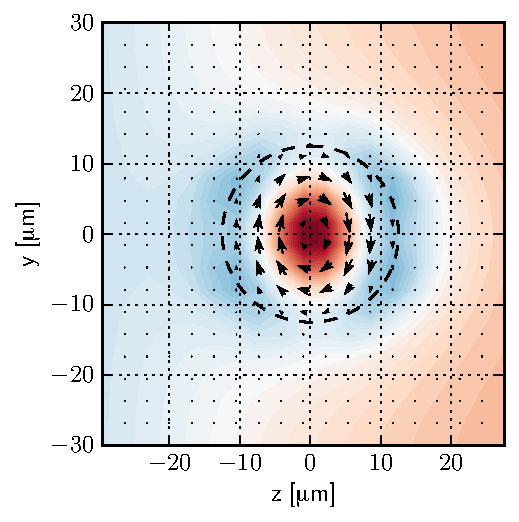
\includegraphics[width=6cm]{img/sphere_Mie_mode_electric.pdf} 
 \centering 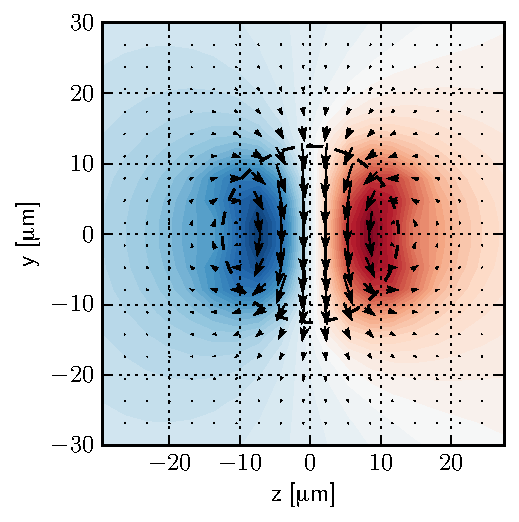
\includegraphics[width=6cm]{img/sphere_Mie_mode_magnetic.pdf} \end{figure}


\add{
Dielectric spheres are delimited in all three dimensions, but they have much in common with the dielectric rods. Their behaviour is closer to that of the rods with orientation parallel to the \textit{magnetic field}. The reason is that the lowest-frequency resonance of both structures is generally the magnetic one, whose circulating electric field is localised in the high-permittivity volume of the particle. Higher resonances require a significant part of the electric field to pass through surrounding air.

In contrast with the previous treatment, we used a realistic model \cite{baumard1977_epsilon_TiO2} of rutile (TiO$_{2}$) for the FDTD simulations presented here to illustrate the effect of losses. The permittivity of the spheres was $\varepsilon^{\text{(1 THz)}} = 94.2+2.43\text{i}$, their diameter was set to $r=30\;\upmu$m  and their spacing along each axis was $a =100$ $\upmu$m. The resulting spectra of reflection, transmission and effective parameters are in Fig. %\ref{fg_spheres_fdtd}a.  XXX
A strong magnetic resonance is apparent at 330 GHz, followed by a weaker electric one at 480 GHz and another magnetic one at 670 GHz. Further resonances are gradually less visible due to lower dipole moment and also due to dielectric losses that increase with frequency. 
For completeness, we extend the frequency axis near $a/(2c) \approx 1.5$ THz, where the first Brillouin zone is reached and a classical Bragg band gap is formed.
The main difference compared to the lossless resonances discussed above (cf. Fig.~\ref{fg_rodh_fdtd}) is the continuous index of refraction, that prevents the index of refraction $N'$ near individual resonances to reach the Brillouin zone boundaries and to form clear edges of the bands. As a result, all effective parameters are continuous even near resonances and do not form separate branches.

An important property of the periodic sphere array is its \textit{isotropic} electromagnetic behaviour. It trivially follows from symmetry under any orthogonal rotation, and it also holds almost exactly under any other orientation (unless the spheres are not touching or too high frequencies are studied).

The right plot in Fig. % \ref{fg_spheres_fdtd}b XXX
shows simulation results for the sphere array interlaced with a wire mesh. The wires are directed along the $x$-axis and $y$-axis, the latter orientation being included only to maintain isotropy of the structure. The wires along the $x$-axis, i.e. parallel to the electric field, have a great impact on the spectra. Most importantly, the structure is now highly reflective at low frequencies, and the resonances introduce transmission windows. (Note the previously discussed sphere array acted in opposite way!) The explanation is contained in the effective permittivity plot, where the wires introduce a region of $\varepsilon_{\text{eff}} < 0$  ranging from 0 to ca 900 GHz. More detailed study of this phenomenon is in the following section. %% which one?

The magnetic resonance introduces narrow regions where $\mu_{\text{eff}} < 0$, thus leading to $N'_{\text{eff}} < 0$ and a propagation mode would occur \cite{dominec2013resonant}. The electric resonance can, on the other hand, overpower the effect of wires so that $\varepsilon_{\text{eff}} > 0$, forming a narrow band with $N'_{\text{eff}} > 0$.
%In practice the resonances are highly lossy, so only the first magnetic resonance introduces a band where the wave can propagate through several cells without being too damped. 

We performed series of experiments to measure the effective permeability  $\mu_{\text{eff}}$ spectrum in a real sample with mean sphere radius of ca. $42\;\upmu$m. The statistical deviation of the resonators size $\sigma \approx 5\;\upmu$m in the sample was unfortunately relatively broad, as was determined by means of microscopy and digital image processing. In contrast to simulations, we were able to constraint the spheres' positions to a plane only, while arranging them in a square array appeared unrealistic. We could anyway compute the single-cell permeability spectra (i. e. the yellow curve in Fig. \ref{fg_experimentalConv}) for many different resonator sizes and add them up. The resulting weighted average (blue curve) then matches the experimental data (red dots) nearly exactly. It shall be however noted that the averaged real part of $\mu_{\text{eff}}$ remained positive even with the best sieving results obtained so far.
\begin{figure}[ht]  \caption{Comparison of the effective permeability of ideal monodisperse sphere array (yellow), weighted average according to the size distribution (blue) and experimental data (red dots).}
\label{fg_experimentalConv} \centering 
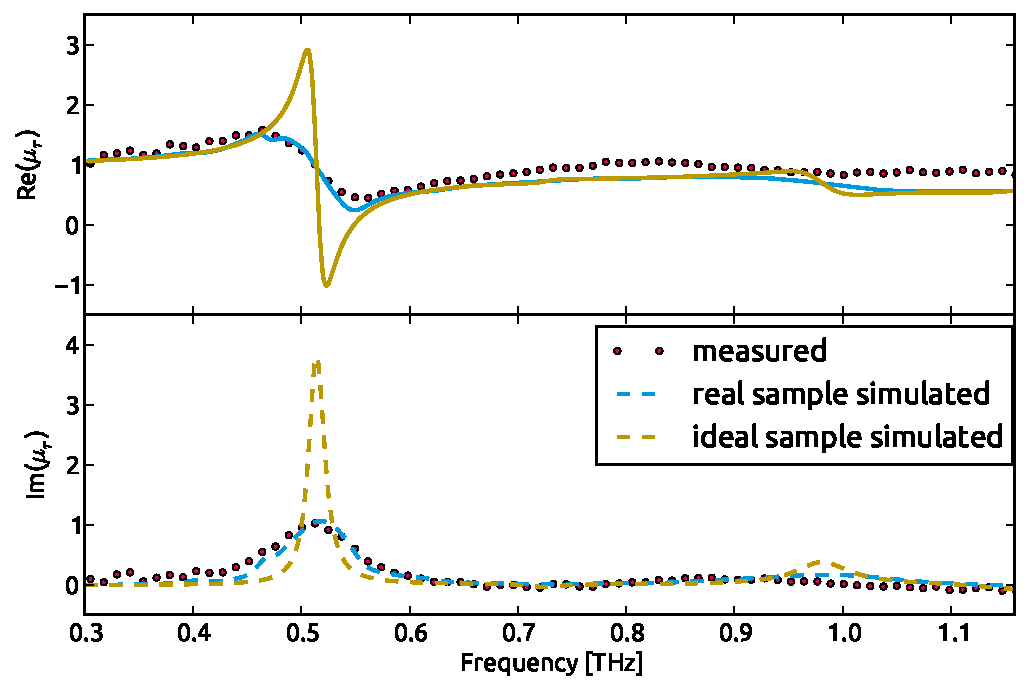
\includegraphics[width=12cm]{img/Spheres_FDTD_experimentalConv.pdf}
\end{figure}
}
\paragraph{Antiresonances and problems with local effective parameters}
% todo refer to the loss scan here

\begin{displayquote}
\textit{antiresonance "may not" come from periodicity, as it is also observed in random structures}  (Ref. \cite{wallen2010})
\end{displayquote}
Anti-resonant curve  of resonant inclusions : ""; %% 
% -- but this argument assumes that aperiodicity  will always prohibit antiresonance; in fact it may just broaden it in spectra
Restoring the physical meaning of MM cosstitutive parameters %%  \cite{alu2010}

%}}}
%% TODO? E-mail: Add the x, y, z, size scans of the ellipsoids%{{{
%> On 19 Mar 2014, at 15:57, <dominecf@fzu.cz>
%> wrote:
%>
%>> Dear Oleg and all,
%>> the frequency dependence of the Mie modes in an ellipsoid is
%>> nontrivial.
%>> Maybe some skilled mathematician could find the analytic expression,
%>> but I
%>> guess its evaluation would require a computer anyway. As an interesting
%>> numerical experiment with FDTD, I ran three scans over the X-, Y- and
%>> Z-
%>> semiaxes of a TiO2 ellipsoid, fixing the remaining semiaxes to 15 um.
%>> The
%>> ellipsoid's X-axis was oriented parallel to the electric field, the
%>> Z-axis
%>> pointed in the wave propagation direction.
%>>
%>> The results attached, best expressed by the dielectric loss spectra in
%>> bilogarithmic plot, show that the first (magnetic) mode is roughly
%>> proportional to X**(-0.4) and Z**(-0.4), while the dependence on the
%>> Y-size is even slower, similar to Y**(-0.2).
%>>
%>> The second Mie mode is more sensitive to the Z-size as Z**(-0.7), while
%>> the other sizes scale very slowly, X**(-0.15), Y**(-0.15).
%>>
%>> In all cases, the exponents of X, Y and Z~dependencies should sum up to
%>> -1, which is the obvious rule for the frequency dependence when all
%>> axes
%>> are scaled simultaneously!
%>>
%>> Note that these estimated exponents are roughly valid only near the
%>> spherical shape, ie. when X~Y~Z. As a matter of fact, the tuning curves
%>> are not straight in the log-log plots. Naturally when one ellipsoid
%>> dimension is much lower than the other two, its role becomes more
%>> pronounced.
%>>
%>> Now we are coming to the big conclusion: Near the spherical shape, the
%>> difference of exponential slope between X- and Y- elongation is
%>> (0.4-0.2)=0.2. Therefore, (15./12.)**(0.4-0.2) gives a reasonable
%>> factor
%>> of 1.0456 difference for the resonant frequencies of the magnetic mode.%}}}
%TODO Note that the effect of mm-phc transition can be also observed in silicon microcubes (thz operation)%{{{
%Planar all-silicon metamaterial for terahertz applications
%@article{prosvirnin2015planar,
  %title={Planar all-silicon metamaterial for terahertz applications},
  %author={Prosvirnin, Sergey L and Dmitriev, Victor A and Kuleshov, Yeugenii M and Khardikov, Vyacheslav V},
  %journal={Applied Optics},
  %volume={54},
  %number={13},
  %pages={3986--3990},
  %year={2015},
  %publisher={Optical Society of America}
%}
%}}}





%====================================================================================================
\section{SRRs and spheres in a wire array or grid} % references to ->
% Cai_Zhu2008-Diel_resonators_wires.pdf
%{{{
\begin{figure} \caption{SphereWire sketch}  \centering  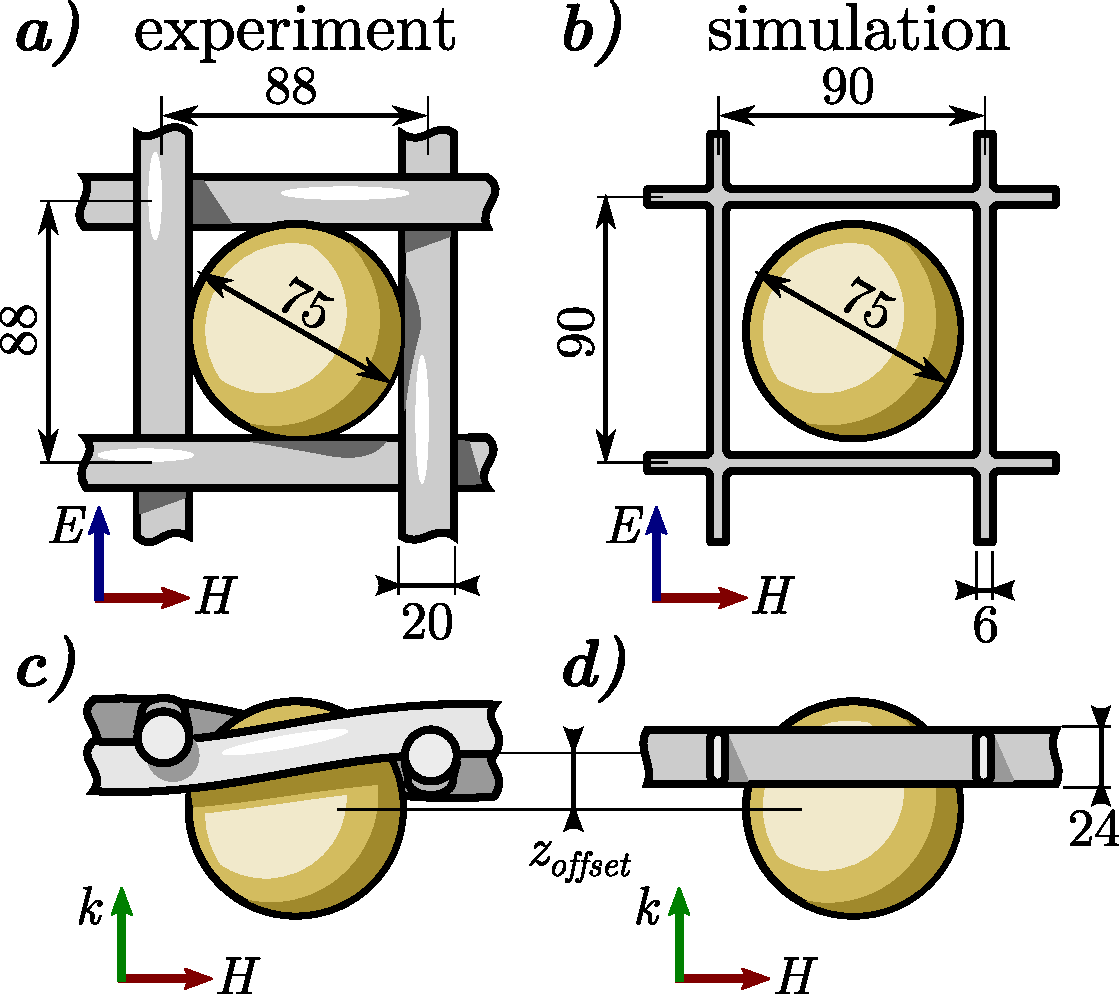
\includegraphics[width=10cm]{img/SphereWire_sketch.pdf} \end{figure} \clearpage

% approximation for frequency well below the grid-resonance  

% 
An elaborate comparison of resonant metallic structures, with clear effect of adding the wire to the transmission spectra, can be found e.g. in Ref. \cite{koschny2004effective}.
%TODO Bitzer2011-Babinet_principle_SRR.pdf

%}}}
\begin{figure}[t] \caption{Amplitude of \textbf{(a)} reflectance, \textbf{(b)} transmittance and \textbf{(c)} effective index of refraction $\Neff = \Neff' + \ii \Neff''$ of TiO$_{2}$ spheres, wire grid array, a combined negative-index structure and its modification  with varied loss compared to the natural one from Ref. \cite{baumard1977_epsilon_TiO2}; sphere radius $r = 30 \upmu$m, unit cell size $a=100$ $\upmu$m.} \label{fg_SphereWire_principles} \centering \vspace{-3mm} %% TODO
\begin{tabular}{r}
\begin{overpic}[width=0.85\textwidth]{img-meep/SphereWire_principles_r.pdf}  \put (-1,28) {\textbf{(a)}} \end{overpic}\vspace{-10.5mm}\\
\begin{overpic}[width=0.85\textwidth]{img-meep/SphereWire_principles_t.pdf}  \put (-1,28) {\textbf{(b)}} \end{overpic}\vspace{-9.5mm}\\
\begin{overpic}[width=0.85\textwidth]{img-meep/SphereWire_principles_n.pdf}  \put (-1,28) {\textbf{(c)}} \end{overpic}\vspace{-9.5mm}\\
\begin{overpic}[width=0.85\textwidth]{img-meep/SphereWire_principles_eps.pdf}\put (-1,28) {\textbf{(d)}} \end{overpic}\vspace{-9.5mm}\\
\begin{overpic}[width=0.85\textwidth]{img-meep/SphereWire_principles_mu.pdf} \put (-1,28) {\textbf{(e)}} \end{overpic}\vspace{-8mm}\\
\end{tabular}
\end{figure}
\clearpage

% TODO
%\ref{fg_SphereWire_principles}


%====================================================================================================
\section{Dielectric rods parallel to magnetic field} % references to ->
\label{sect_diel_rods_mag}
\add{Such a behaviour at the lower and upper boundaries of the band gap is typical of classical \textit{Bragg} band gaps; individual resonances in other types of structures result in change of $K$ and	introduce more complex differences between the field shape.}
%{{{

analytic shape of the Mie resonance, \cite{obrien2002photonic} 

\add{
 The operation of all sorts of left-handed metamaterials  relies on  the \textit{internal resonances} based on non-propagating evanescent fields in the structure. We conjecture such resonances may never occur in 1-D dielectric structures, so their study requires a simulation of a 2-D or 3-D structure.
% Todo elaborate the idea of nonBragg gap <-> nonradiative fields in structure <-> permittivity/permeability resonance
% Note that in 1-D dielectric PhC, all fields are propagating, none evanesecnt
% Big question: Can one approximate a metamaterial by ENG/DNG/MNG/DPS 1-D PhC??
\begin{figure}[ht] \caption{Dispersion curves for dielectric rods aligned parallel to magnetic field. The side plots show the shape of the fields in the $(x,z)$ plane, at the frequencies of the band edges. The magnetic field is plotted as color map and the electric field is represented by vectors. The rod radius was chosen to 12 \% of the period. \textbf{(a)} On the left, a relatively low permittivity $\varepsilon = 12$ places the magnetic resonance above the first Bragg band gap. \textbf{(b)} For high permittivity dielectric $\varepsilon = 100$, the magnetic resonance forms the first band gap. } \label{fg_rodh} \centering 
\textbf{(a)}	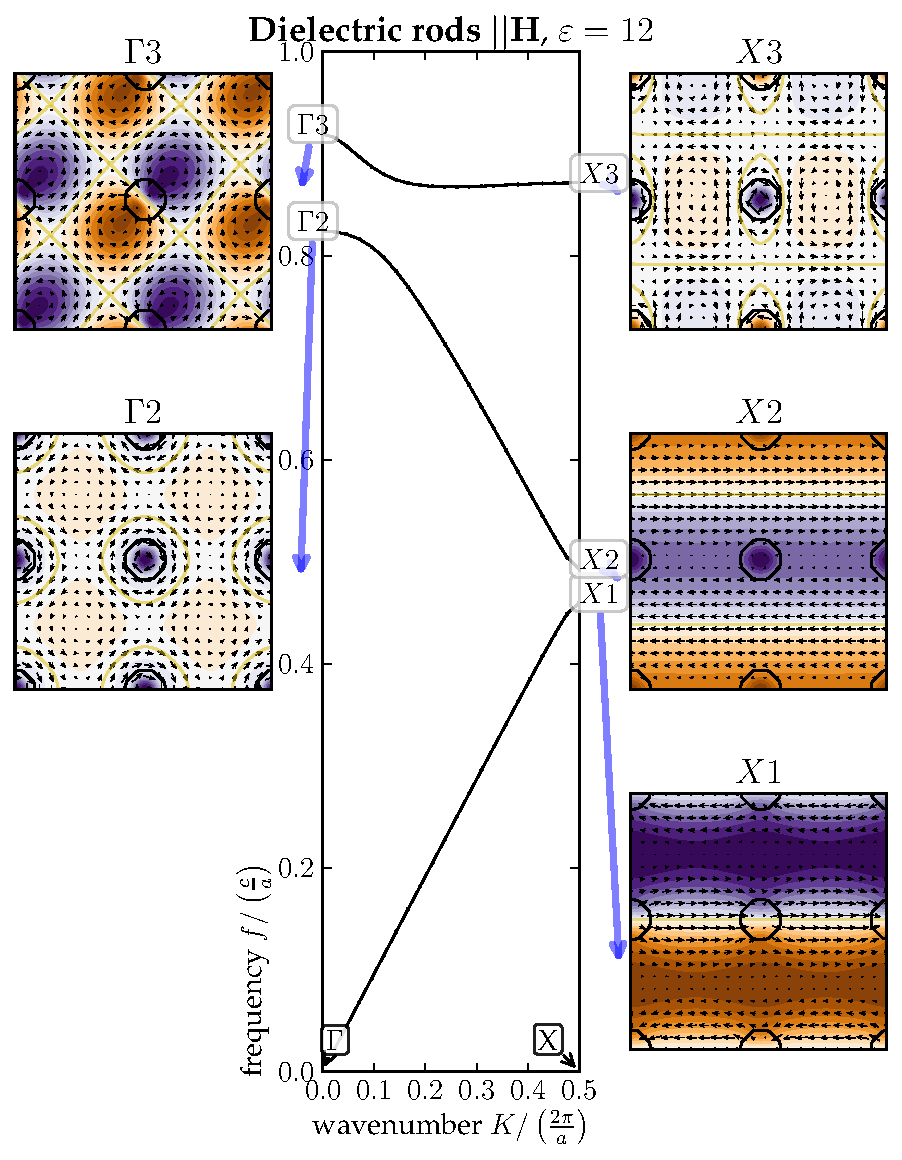
\includegraphics[width=.45\textwidth]{img/HRods_eps012_R12_PWEM.pdf}
\textbf{(b)}	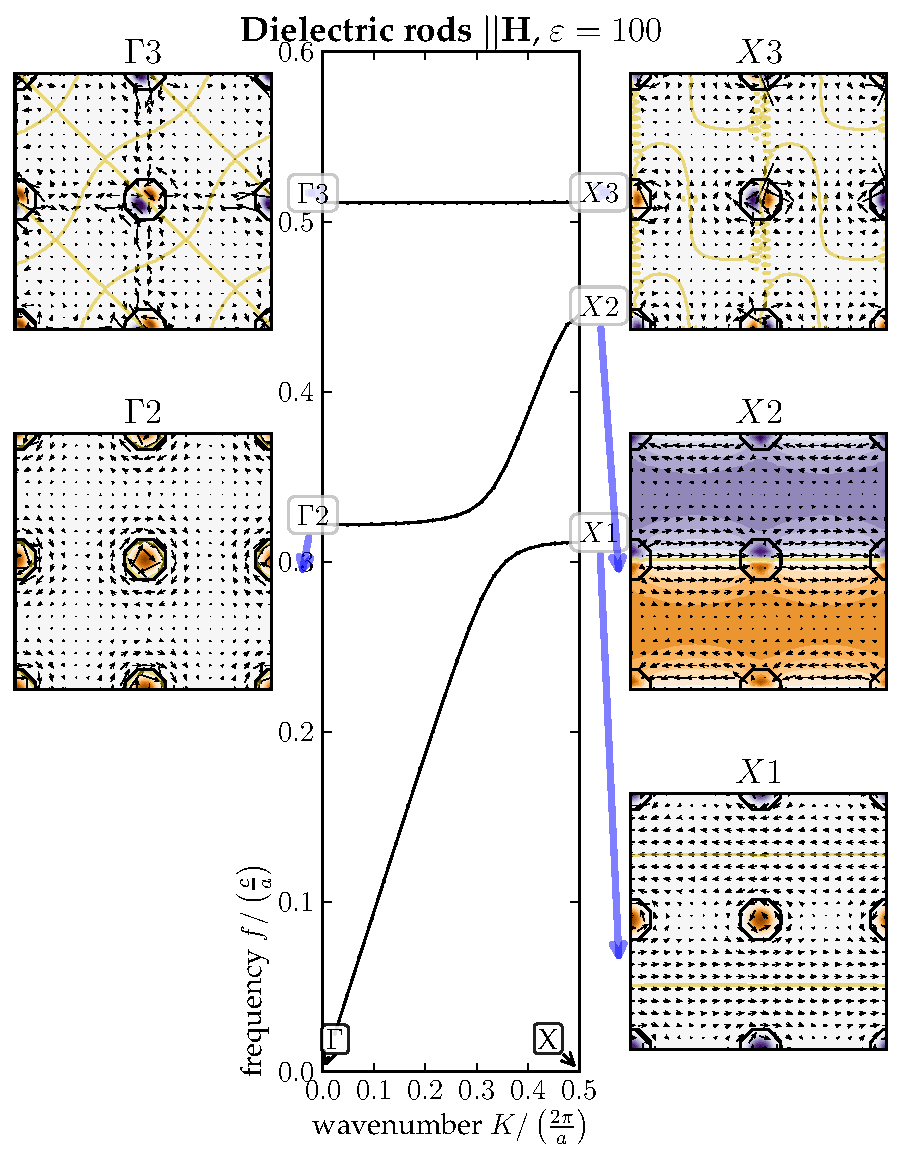
\includegraphics[width=.45\textwidth]{img/HRods_eps100_R12_PWEM.pdf}
\end{figure} %% TODO OVERPIC

Probably the simplest example of such structures is a periodic array of high-permittivity dielectric rods, aligned parallel to the $y$-axis. (We use the convention that the structure is excited by a plane wave source with $\mathbf E || \mathbf x$, $\mathbf H || \mathbf y$ and the wave propagates along the $z$-axis). % dubious - the E, H have many directions in the unit cell; better  to write "TM"/"TE"? But this would confuse with nonperp incidence!
The inhomogeneity of the structure along the $x$-axis allows the electric field to circulate along the rod -- or, more precisely, the $\mathbf E$ field can now be decomposed into purely \textit{planar} part known from the previous section, %% TODO which one?
and a purely \textit{circulating} part, that induces a magnetic flux near the rod axis. The circulating electric field is clearly visible on both plots in Fig. \ref{fg_rodh}, where all nonzero components of the fields ($H_y$, $E_x$ and $E_z$) are depicted. 

% discuss why this is not true: each lorentzian introduces delta mu -> so the low-frequency permeability of rod array should be > 1? Attracted to a magnet?
This new type of resonance is known as a \textit{magnetic Mie resonance}, \cite{obrien2002photonic, nemec2009tunable, yahiaoui2009broadband, yahiaoui2011tunable}. Unlike the Bragg gaps, it can be observed also in a single rod in free space. Being a function of the frequency of the incident wave, the magnetic dipole moment of the free-standing dielectric rod follows the characteristic Lorentzian shape of its \textit{resonance curve}. Below the resonance the magnetic dipole moment of the resonator goes to strongly positive values, while in a narrow region above the resonance it is strongly negative. How does this behaviour change if we arrange the rods in an infinite periodic array? 


The results from a PWEM computation are plot in Fig. \ref{fg_rodh}. To obtain comparable dispersion curves in Fig. \ref{fg_rodh_fdtd}, we employed the FDTD simulation and the effective parameter retrieval described above. The main differences are that in Fig. \ref{fg_rodh_fdtd} we plot the frequency $f$ on the horizontal axis and we also use the effective index of refraction $N_{\text{eff}} := K\cdot \frac{c}{2\pi\,f}$ instead of the wavenumber $K$. One advantage of this representation is that $N_{\text{eff}}$ should be compliant with the Kramers-Kronig relations. This criterion always gives \textit{only one} correct solution on how to unfold $K$ to obtain realistic $N_{\text{eff}}$. 
In the simulation, the rod spacing (or, lattice constant) $a$ was 100 $\upmu$m, so the normalised frequency unit is $c/a = 3$ THz. The frequency range from 0 to 1.8 THz was therefore chosen the same as in Fig. \ref{fg_rodh}b. 
Note the first resonance shows pronounced resonant shape in the plot of permeability, which is typical of magnetic Mie resonances. In a very narrow region 960-970 GHz, the permeability $\mu_{\text{eff}}$ is real and negative. 
Apart from $N_{\text{eff}}$, the FDTD computation gives also the effective wave impedance $Z_{\text{eff}}$, which is a complementary information we need to compute the effective permittivity $\varepsilon_{\text{eff}}$ and the effective permeability $\mu_{\text{eff}}$:

\begin{equation} \varepsilon_{\text{eff}} = N_{\text{eff}}/Z_{\text{eff}}, \quad\quad\quad\quad \mu_{\text{eff}} = N_{\text{eff}}\cdot Z_{\text{eff}}.
\label{eq_epsmu}\end{equation}

\begin{figure}[ht]  \caption{Effective parameters of an array of dielectric rods $||\mathbf H$ with same parameters as in Fig. \ref{fg_rodh}b (i.e. radius of  12 \% of the period and permittivity $\varepsilon = 100$). Complex reflection $r$ and transmission $t$ spectra allow to compute the effective index of refraction, impedance (not shown), permittivity and permeability. Thin grey lines indicate the Brillouin zone boundaries.}
\label{fg_rodh_fdtd} \centering 
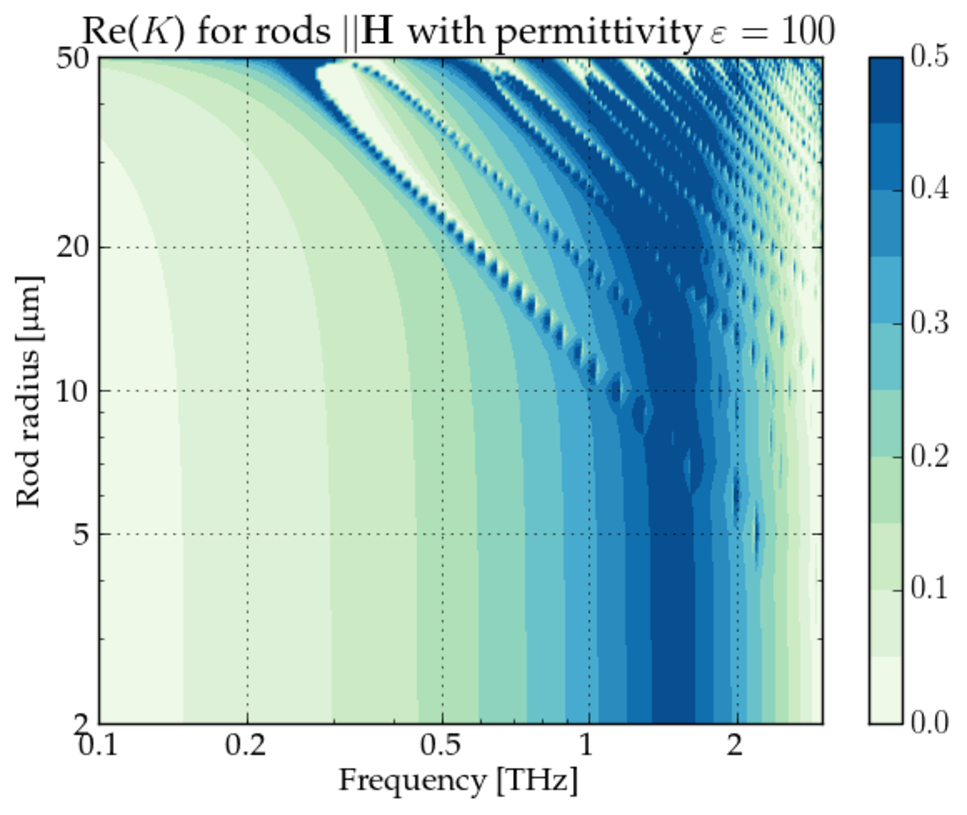
\includegraphics[width=8cm]{img/old/HRods_eps100_radiusscan.pdf}
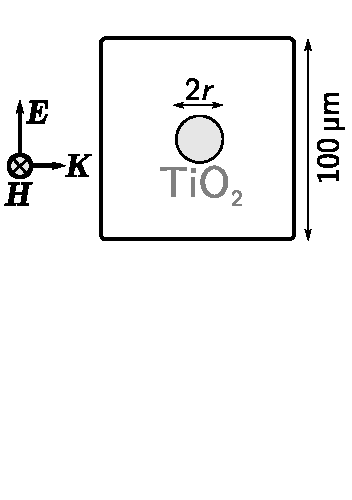
\includegraphics[width=4.5cm]{img/HRods_sketch.pdf}
\end{figure}

Other Mie resonances are located at higher frequencies. As a general rule for similar structures, the odd-numbered resonances have magnetic dipole moment (along the rod axis), whereas the even-numbered resonances have electric dipole moment (perpendicular to the rod axis). The reason is that electric dipole moments in odd resonances are suppressed due to antisymmetric shape of the mode; naturally the same holds for the magnetic moments in the even resonances.

The frequency of the Mie resonances is not significantly influenced by the photonic bands. Therefore, in order to understand the resulting band structure and its dependence on parameters, one has to disentangle which band gaps are due to Bragg reflection and which correspond to magnetic or electric Mie resonances. This is much easier knowing the spectra of $\varepsilon_{\text{eff}}$ and $\mu_{\text{eff}}$, as provided by FDTD in Fig. \ref{fg_rodh_fdtd}.
\begin{figure}[ht] \caption{The spectra of the wavenumber $K$ for different rod radii and two different rod permittivities. The wavenumber plot is folded so it ranges from 0 to 0.5, where $K\approx 0$ and $K\approx 0.5$ correspond to band gaps. \textbf{(a)} Medium-permittivity rods with $\varepsilon = 12$, \textbf{(b)} high-permittivity rods with $\varepsilon = 100$.  } \label{fg_hbar_radiusscan} \centering 
\textbf{(a)}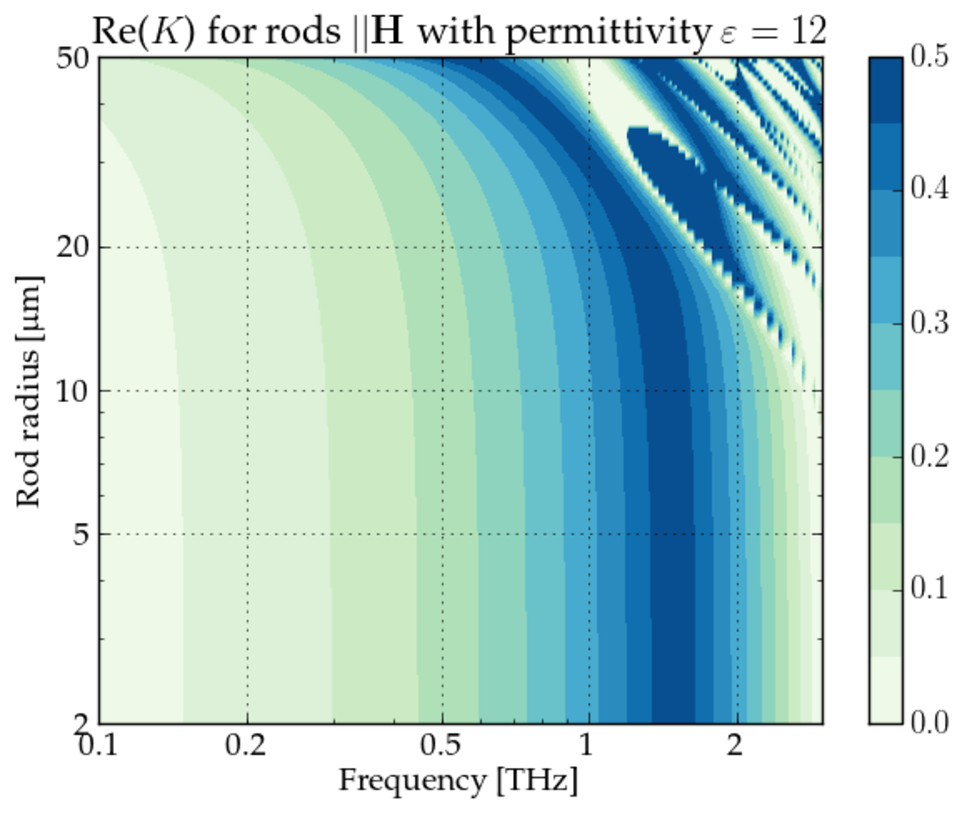
\includegraphics[width=8cm]{img/old/HRods_eps012_radiusscan.pdf}
\textbf{(b)}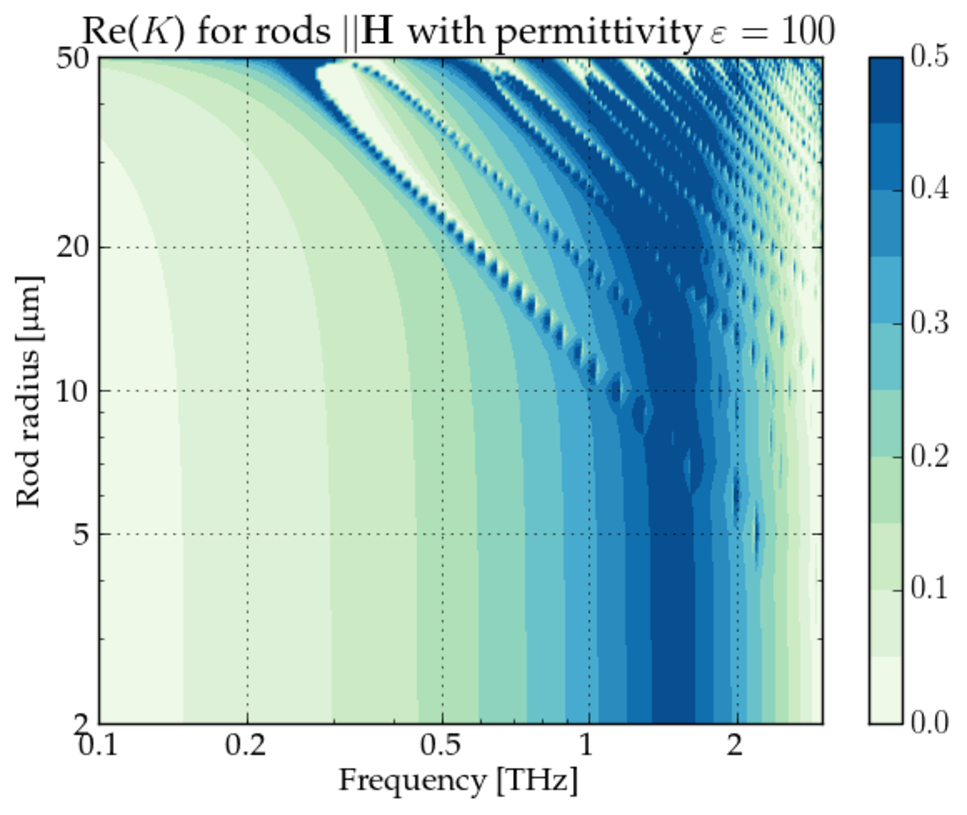
\includegraphics[width=8cm]{img/old/HRods_eps100_radiusscan.pdf}
\end{figure}

The photonic crystals composed of square lattice of dielectric rods have been examined thoroughly since early 90s \cite{plihal1991two, pendry1992_transfer_matrix}. The permittivity of the constituent materials was rather low, corresponding to the optical or near-infrared frequencies, where the suitable materials usually have permittivity $\varepsilon < 12$. By parametric scans we could prove that for rod permittivity below 60 or even 80, the individual resonance is always located at higher frequency than the Bragg gap. Little, if any, attention was therefore paid to different nature of the higher resonances and most publications focused on properties and applications of the Bragg band gap.

The situation is different in the terahertz range, as the lattice of the crystalline solids often exhibits optical phonons at frequencies between 5 and 20 THz. The permittivity of many materials turns out to be much higher for frequencies below these resonances. This enables to conceive structures composed e.g. of titanium dioxide \cite{baumard1977_epsilon_TiO2} with $\varepsilon^{\text{THz}} \approx 92$ or of ferroelectrics with $\varepsilon^{\text{THz}}$ even orders of magnitude higher \cite{skoromets2011tuning}. The price to be paid for this advantage in the THz range are the relatively high losses caused by the lattice vibrations.

\begin{figure}[ht] \caption{Behaviour of the rods $||\mathbf E$, with permittivity $\varepsilon = 100$ and radius $r=11\;\upmu$m.\\
\textbf{(a)} Band diagram and modes from PWEM. 
} \label{fg_erod_radius11} \centering 
\textbf{(a)}	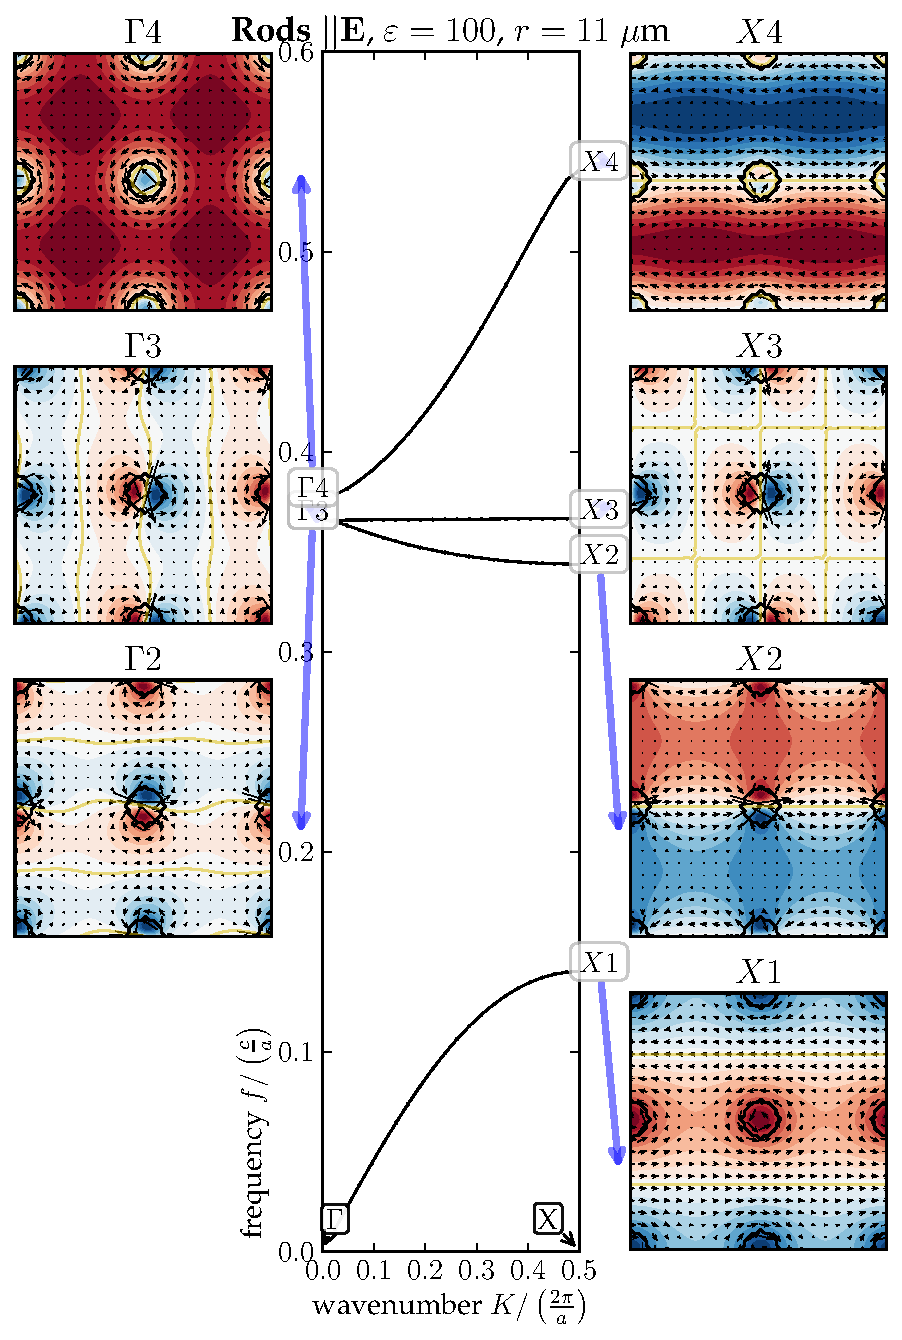
\includegraphics[width=8.5cm]{img/ERods_eps100_R11_PWEM.pdf}
\end{figure}

}

%}}}





%====================================================================================================
\section{Dielectric rods parallel to the electric field} % references to ->

\label{sect_diel_rods_el}
%{{{
% TODO refereence  also to \cite{valdivia2012} and \cite{shi2007}
\cite{yang2015}




%}}}

%{{{ FROM SHORT.pdf
\mdf{  
\begin{figure}[ht] \caption{The spectra of the wavenumber $K$ for different rod radii and two different rod permittivities, analogical to Fig. \ref{fg_hbar_radiusscan} except for different orientation. \textbf{(a)} Medium-permittivity rods with $\varepsilon = 12$, \textbf{(b)} high-permittivity rods with $\varepsilon = 100$.  } \label{fg_ebar_radiusscan} \centering 
\textbf{(a)}	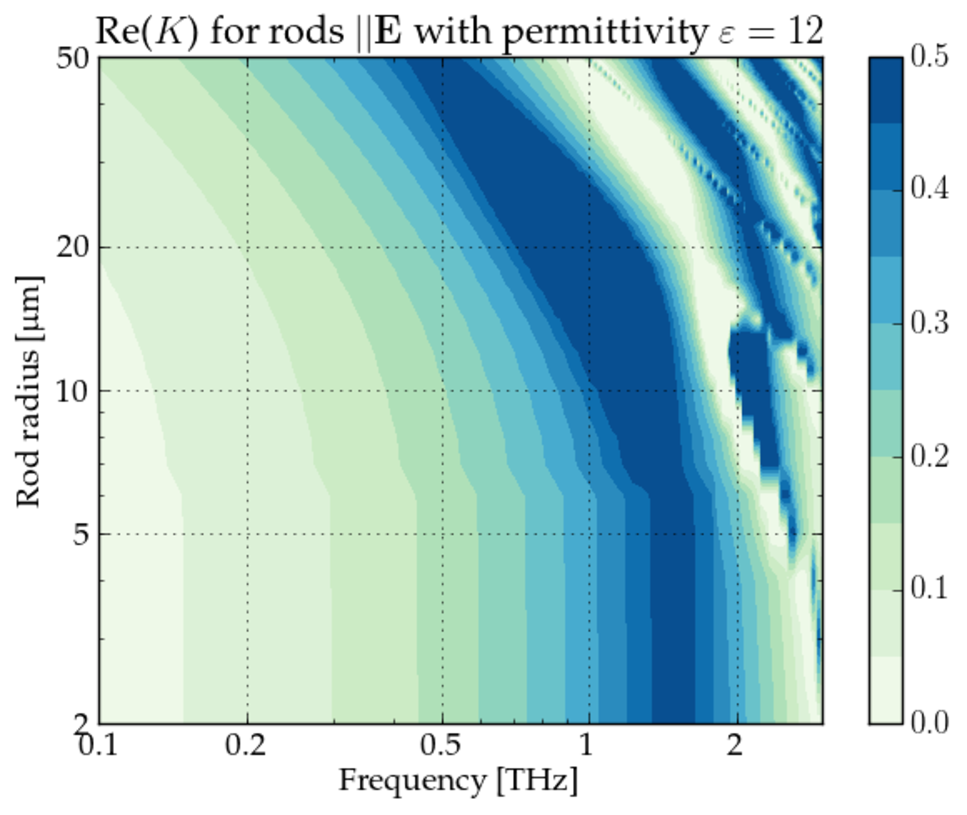
\includegraphics[width=8cm]{img/old/ERods_eps012_radiusscan.pdf}
\textbf{(b)}	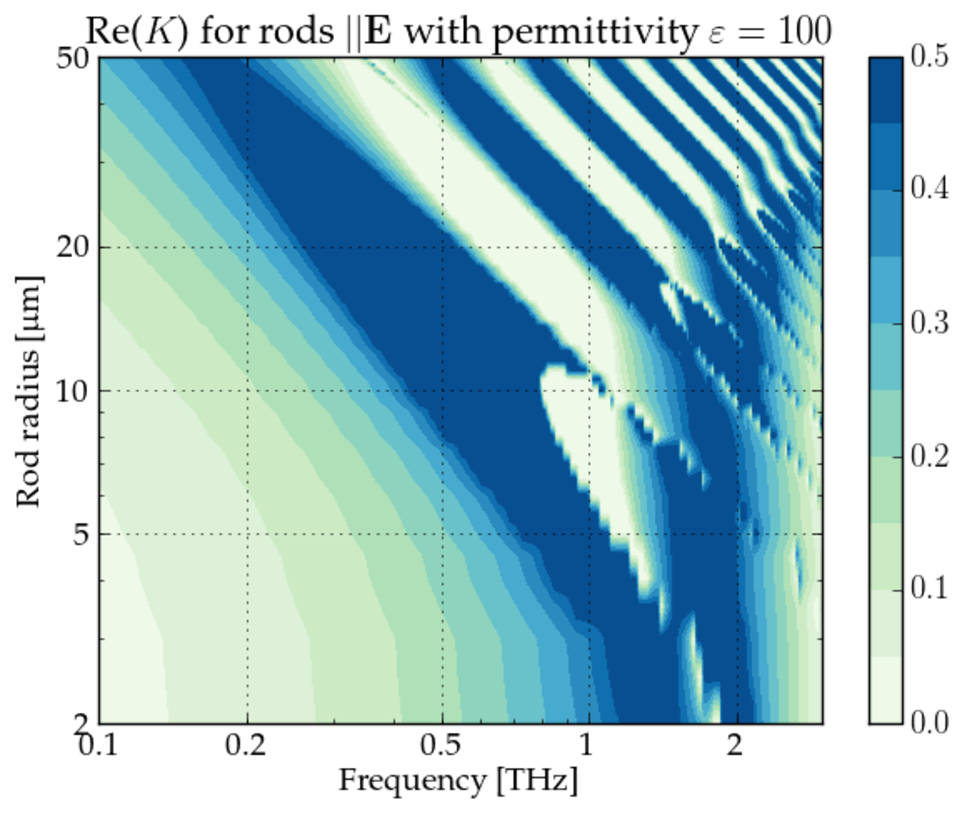
\includegraphics[width=8cm]{img/old/ERods_eps100_radiusscan.pdf}
\end{figure}


The dielectric bars parallel to the electric field represent the same structure as previously discussed, except that it is orthogonally rotated. There is however a qualitative difference in that the high-permittivity dielectric is continuous along the direction of the electric field, so the effect of the dielectric is expected to be much stronger. This results in that the first Mie resonance is the \textit{electric} one. Its overlap with the next magnetic resonance can eventually lead to negative index of refraction in such a structure \cite{peng2007, vynck2009}. If the permittivity of the rods is chosen to be $\varepsilon = 100$ and the periodicity of the lattice $a = 100\;\upmu$m, the negative index of refraction occurs in a narrow range of radii from 9 to 12 $\upmu$m. The behaviour of this structure with the desired radius is depicted in Fig. \ref{fg_erod_radius11}a,b.

In order to form a photonic band with a negative index of refraction, both the permittivity and permeability need to be negative. In the structure discussed, this is made possible by the frequencies of the electric and magnetic Mie resonances being close enough to overlap.
The electric resonance would be surrounded by its broad band gap between the frequencies spanning from $0.13 \cdot\frac{c}{100\;\upmu\text{m}} \approx 400$ GHz to  $0.38 \cdot\frac{c}{100\;\upmu\text{m}} \approx 1140$ GHz. This is also confirmed by Fig. \ref{fg_erod_radius11}a where the mode shapes X1 and $\Gamma$4 perfectly correspond to the electric Mie resonance. 

For the interesting range of radii around 11 $\upmu$m, the magnetic resonance introduces a new, narrow photonic band starting from X2. Now, moving on to the right plot of Fig. \ref{fg_erod_radius11}b, we can clearly identify the resonant frequencies of 815 and 900 GHz. They cause abrupt skips of the refractive index which always shift the index of refraction by one Brillouin zone down.\footnote{The individual resonance appears to be the only mechanism that causes $N'_{\text{eff}}$ to \textit{decrease} in the spectrum. In photonic bands, no matter if $N_{\text{eff}} > 0$  or $N_{\text{eff}} < 0$, the real part of $N_{\text{eff}}$ always grows in accordance with the Foster theorem. This is confirmed by the FDTD results and by their compliance to Kramers-Kronig relations. To illustrate this, the Hilbert transform of the refractive index is plotted as the thin pink line and it nearly perfectly follows the green curve over whole spectrum, except for an additive constant. There is  only one acceptable physical solution that is compatible with the Kramers-Kronig relations.}
The resonance is accompanied by a sharp peak in the imaginary part of refractive index $N''$ and by transmission amplitude touching zero ($|t| = 0$). As both Mie resonances precede the Bragg gap, the index of refraction is pushed into negative values and the following photonic band gap $N' < 0$.

For completeness we add the FDTD results with effective permittivity and permeability, computed for the entire spectrum. These quantities however seem to have a useful physical interpretation only within the photonic bands, or within those parts of the photonic band gaps where $N = 0$. 
\\

The dispersion curves of the rods with radii different than 11 $\upmu$m are compared in Fig. \ref{fg_ebar_radiusscan}b based on multiple FDTD simulations. The individual resonances are again easy to be distinguished by abrupt changes from white to blue or vice versa (i.e. skips between the Brillouin zones). We can see that for radii below 8 $\upmu$m the magnetic resonance is at too high frequencies, forming its separate band gap. For even thinner rods at the very bottom edge of the plot, no individual resonance intersects with the first Bragg  band gap at all. 

An interesting qualitative change of the structure response occurs when the rods get slightly thicker than discussed above, say $r > 12\;\upmu$m. The electric and magnetic resonance frequencies do never cross over, but instead they  and an ordinary Bragg band gap remains. The transmission curve of single cell (Fig. \ref{fg_erod_radius11}) continuously shifts up and does not touch zero anymore. We may conclude that for rod radius being too high, the structure no more exhibits the negative index of refraction and starts to behave similar to the 1-D photonic crystal discussed above.
% TODO explanation by nodal planes

%The dependence of the folded wavenumber $\text{Re}(K)$ for high-permittivity rods $||\mathbf E$ is plotted in Fig. \ref{fg_ebar_radiusscan}b. Starting from very thin rods ($r=2$ \um) at the very bottom of the plot, we can see the first band gap (1.3 to 1.5 THz) denoted by darkest blue is purely of the Bragg type, followed by a 

Comparing the low-permittivity and high-permittivity cases in Fig. \ref{fg_ebar_radiusscan}a,b, one can see there exists some minimum limit for the permittivity contrast that is necessary for both electric and magnetic resonances to be located in the first gap simultaneously. We determined this scale-invariant value to be roughly 80.

The transmission peaks can be clearly identified with resonant modes and it was observed that the frequencies of the modes shift with different slope depending on parameters.  
} 
%}}}




\begin{figure} \centering 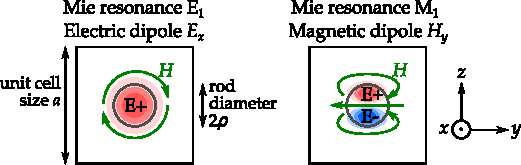
\includegraphics[width=14cm]{img/ERods_1st_and_2nd_Mie_resonance.pdf}%{{{
\caption{(a) Perspective view of the unit cell\add{; (b) its} cross-sections with the resonant modes excited by a plane wave with $\mathbf{E}||x, \mathbf{H}||y$ and $\mathbf{k}||z$. The first Mie resonance has an electric dipole moment only, while the second one has a magnetic dipole moment instead. The red and blue color shows positive and negative values of the $E_x$ component of the electric field, while the magnetic field is represented by the arrows. } \label{fg_sketchfield} \end{figure}

Our structure \add{(see Fig.\ref{fg_sketchfield}a)} is defined by a square unit cell with the linear dimension $a$ periodically distributed in the $yz$ plane; the dielectric rod parallel to $x$-axis with radius $\rho$ and permittivity $\varepsilon_r$ is positioned in its center. We employed the finite-difference time-domain (FDTD) simulation package MEEP \cite{oskooi2010meep} to obtain the scattering coefficients (complex reflectance $r$ and transmittance $t$) of a structure with variable number of unit cells along the wave vector direction $k\parallel z$. The incident wave is polarized $E\parallel x$, periodic boundary conditions were applied in the $y$-direction. We performed the simulations for a single layer ($y$-periodic boundary conditions only). Its effective properties are almost identical to those of the corresponding multilayer structure. We checked that for this geometry, the retrieved effective parameters depend only negligibly on the number of unit cells in the $z$-direction. The relevance of the calculations with a single layer was further confirmed by current-driven homogenization simulations \cite{markel2013current} in several particular cases (same geometries as in Fig.~\ref{fg_spec}) which yielded a response in a very good agreement with the FDTD results.

The effective parameters were \add{then} retrieved from complex transmittance and reflectance spectra \cite{smith2002determination}.  \add{Alternative means of obtaining the effective parameters are discussed in Ref. \cite{simovski2009material}. When inverting the Fresnel-Airy formulas, the correct solutions have to be chosen in the different parts of the $\Neff(\omega)$, $\Zeff(\omega)$ spectra \cite{simovski2009material}; to this aim, Kramers-Kronig relations as well as the conditions of a passive medium Im$(\Neff)>0$ and Re$(\Zeff)>0$ were used.} 

The retrieved value of the complex effective index of refraction $\Neff(f)$ defines the magnitude of the wave vector
\begin{equation}\label{eq_wave_vector} k(f) = 2\pi f \Neff(f) /c\,.  \end{equation}
Note that the retrieval procedure  implies that the wave vector introduced by Eq. (\ref{eq_wave_vector}) is defined in an unfolded reciprocal space. 

A Bragg resonance occurs when an integer number of half-wavelengths fit into one unit cell, i.e.,  when
\begin{equation}\label{eq_BZ} k(f) = \frac{q \pi}{a}\,, \end{equation}
where $q$ is a non-zero integer. In such a situation, the wave vector is located at a Brillouin zone boundary. The purely real values of $k$ then describe photonic band edges.  In a band edge state, a standing wave appears in the structure and it is characterized by exactly $q$ nodal planes dividing each unit cell in the transverse direction to $q+1$ disconnected parts. The band edges delimit a photonic {\itshape Bragg band gap} where only evanescent waves described by $\Neff''>0$ can exist.  We can write an equation analogous to (\ref{eq_BZ}) for the real part of the refractive index:
\begin{equation}\label{eq_BZN} \Neff'(f) = \frac{q c}{2 a f}\,; \end{equation}
its hyperbolic behavior versus frequency reflects the pinning of the wave vector to the Brillouin zone boundary inside the Bragg band gap.

Another case of interest where evanescent waves are obtained is that of $\Neff' = 0$ (center of the first Brillouin zone, $q=0$) and $\Neff''>0$. Here the waves exponentially decay in the medium without any phase change. However, this behavior has a different origin: it is connected to a plasma-like response of the material ($\varepsilon<0$ or $\mu<0$) and in this paper we use the term \textit{plasma band gap} to refer to it.

The Kramers-Kronig relations require that for any structure studied, $\Neff'(f)$ [or, equivalently, $k(f)$] attains and finally crosses the Brillouin-zone boundaries when the frequency is sufficiently increased. While usually the convention is used that the corresponding curves are folded back into the first Brillouin zone, in this paper we plot $\Neff'(f)$ in the original (unfolded) Brillouin zones resulting from the retrieval algorithm. This can be clearly observed on the dispersion of the refractive index in Fig.\ \ref{fg_spec}. In this way we retain the information about the number of the nodal planes intersecting the unit cell, which is important for our discussion.
%}}}


\todo{FIGURE: Results of the FDTD simulations for a single layer of dielectric rods with $\varepsilon_{\rm r}= 100$, $\rho=10$\,$\upmu$m. The spectra of reflection $|r|$ and transmission $|t|$ amplitudes share their frequency axes with the retrieved complex effective index of refraction $\Neff$, permittivity $\eeff$ and permeability $\meff$, whose imaginary parts are denoted by dashed lines. The frequency ranges where $\eeff$ and $\meff$ have no physical interpretation (Bragg band gaps or higher order photonic bands) are gray shaded.  } 

In the following, we first describe in detail three characteristic cases: we compare the effective parameters computed for three slightly different unit-cell sizes while the rod radius and the dielectric permittivity are fixed. The comparison of these cases reveals quite remarkable changes in the optical behavior of the structure. We then complement this comparison by a continuous scan of the unit-cell sizes in order to obtain an overview of all possible types of the response for the rod-based geometry.  

In Fig.~\ref{fg_spec}, we show the calculated reflectance and transmittance amplitude spectra, as well as the effective parameters of three representative structures which have the same rod radii $\rho = 10$~$\upmu$m, but they differ by the unit-cell size $a =$ 120, 100 and 80 $\upmu$m. These values of $a$ were selected to illustrate three qualitatively different regimes of behavior.  The dielectric was defined by a simple lossy model with one high-frequency oscillator, its  permittivity was $\varepsilon_r = 100.1 + 0.5\mathrm{i}$ at 500 GHz.

\paragraph{Sparse array}
In Fig.~\ref{fg_spec}(a), where the unit-cell size $a=120$~$\upmu$m, we can see two well separated Mie resonances: the electric one at 680 GHz and the magnetic one at 1030 GHz.  The field distribution of the corresponding modes is sketched in Fig.~\ref{fg_sketchfield}. The resonance frequencies can be easily identified by an abrupt drop in the real part of the effective index of refraction $\Neff'$, accompanied by a sharp peak in its imaginary part $\Neff''$. The Mie resonances in periodic media without losses must always be adjacent to a Bragg band gap. For instance, in Fig.~\ref{fg_spec}(a) at frequencies below the first Bragg gap, the electric dipoles within each rod are directed along the electric field in the rest of the unit cell. The rods thus positively contribute to the refractive index $\Neff'$ which progressively grows until it reaches the first Brillouin zone boundary. At this point, the Bragg condition for a photonic band-gap is fulfilled and each unit cell is intersected by one nodal plane. This is reflected by the dispersion of $\Neff'(f)$ which follows the first Brillouin-zone boundary in the first Bragg band gap between 400 and 680\,GHz [equivalent to $q=1$ in Eq. (\ref{eq_BZN})]: $$	\Neff'(f) = \frac{c}{2af}\,. $$ At 680\,GHz, the electric Mie resonance occurs which dramatically changes the near-field photonic properties of the structure. The observed drop in $\Neff'(f)$ and the slope change in $\Neff''(f)$ mark the plasma-like character of the adjacent part of the band gap which extends up to the plasma frequency of the Mie resonance (940\,GHz). In this frequency range the electric dipoles in the rods change their direction and induce an electric field opposite to the incident one.

For this sparse array of dielectric rods, the first magnetic Mie resonance lies at 1030\,GHz, above the plasma frequency of the electric mode.  The second Bragg band-gap opens at 1010 GHz and, due to the Mie resonance, it is transformed to a plasma band gap at 1030 GHz. The next allowed photonic band starts above magnetic plasma frequencies at 1070 GHz. Therefore we observe a very analogous behavior near the magnetic resonance. 

For completeness we note that at 1350 GHz, a third Bragg band gap starts which, unlike the lower-frequency ones, does not contain any Mie resonances [see Fig.\ \ref{fg_spec}(a)].

The resonances in the effective permittivity $\eeff=\Neff/\Zeff$ and permeability $\meff = \Neff\cdot \Zeff$ of a periodic array obviously exhibit shapes very different from the well-known resonance curves of a damped oscillator\cite{koschny2003resonant}. In the two separate plasma band gaps we obtain either $\eeff < 0$ or $\meff<0$, i.e. the usual behavior observed in the reststrahlen bands of resonances. However, in the Bragg band gaps occurring just below these spectral ranges the behavior of $\eeff$ and $\meff$ does not have any useful physical interpretation and it can be understood as a purely formal frequency dependence: we shaded these ranges with light gray in Fig.~\ref{fg_spec}.
%}}}
\paragraph{Medium array}%{{{
When the unit cell size is reduced to $a=100$~$\upmu$m, as depicted in Fig.~\ref{fg_spec}(b), the Mie resonances shift slightly. Interestingly, in comparison with the sparse array, the electric resonance frequency increases from 680 to 780 GHz, and that of the magnetic resonance decreases from 1030 to 980 GHz. This can be explained by the inter-cell coupling: the circulating magnetic field of the first resonance is compressed when the rods get closer, whereas the magnetic dipoles of the second resonance can couple more easily to each other in the same situation (see Fig.~\ref{fg_sketchfield}).

The converging of the resonance frequencies is linked to the most important qualitative change in the spectra: the fact that the magnetic resonance occurs at a frequency where $\eeff'<0$. The first band gap (the lowest continuous frequency region where $\Neff''>0$) is thus composed of three adjacent regimes: the first Bragg band gap (425--780 GHz), a plasma band gap (780--980 GHz) and the second Bragg band gap (980--1020 GHz). Every Mie resonance introduces a drop in $\Neff'$, so the following photonic band (1020--1070 GHz) features a negative index of refraction ($\Neff'<0; \Neff''\approx 0$), i.e., the phase and group velocities are opposite to each other. We conjecture that the presence of two Mie resonances in the \textit{first} combined band gap is a necessary and sufficient condition for $\Neff'<0$ to occur.

Note that the transmittance amplitude reaches quite small values between the Mie resonances when they are sufficiently close to each other [Fig. \ref{fg_spec}(b)]. This range forms a well-defined band with a reflectance-to-transmittance contrast much better than that observed in a planar Fabry-Perot resonator. One layer of dielectric rods with proper parameters can therefore be applied as a thin, yet very effective filter.
%}}}
\paragraph{Dense array}%{{{
Perhaps an even more surprising change occurs when the rod spacing is further reduced. The Mie resonances get even closer in the spectrum and eventually they vanish for $a=80$~$\upmu$m [see Fig.~\ref{fg_spec}(c)]. The band gap remains at nearly the same spectral position as in panel (b) of this figure, but, unlike for the medium array, the value of $\Neff'$ does not drop within the Bragg band gap. In contrast, it is shifted up to the second Brillouin zone boundary where it meets the second Bragg band gap as clearly seen in panel (c), indicating that each unit cell is intersected by two nodal planes in this state.

The reason of this behavior is related to the change of the nodal plane topology caused by the inter-cell coupling. When the rods are far from each other ($a\gtrsim 100$~$\upmu$m), the individual Mie resonances create closed regions delimited by a nodal surface where the fields are opposite to the rest of the unit cell. Upon reducing the unit-cell size ($a\lesssim 80$~$\upmu$m), the regions of opposite fields start to overlap with those from the neighboring cells and the corresponding nodal surfaces interconnect and open. This pair of open nodal surfaces dividing the unit cell manifests itself by a qualitative change of the $\Neff'$ spectrum towards a shape typical for one-dimensional photonic crystals.

\begin{figure}\centering 
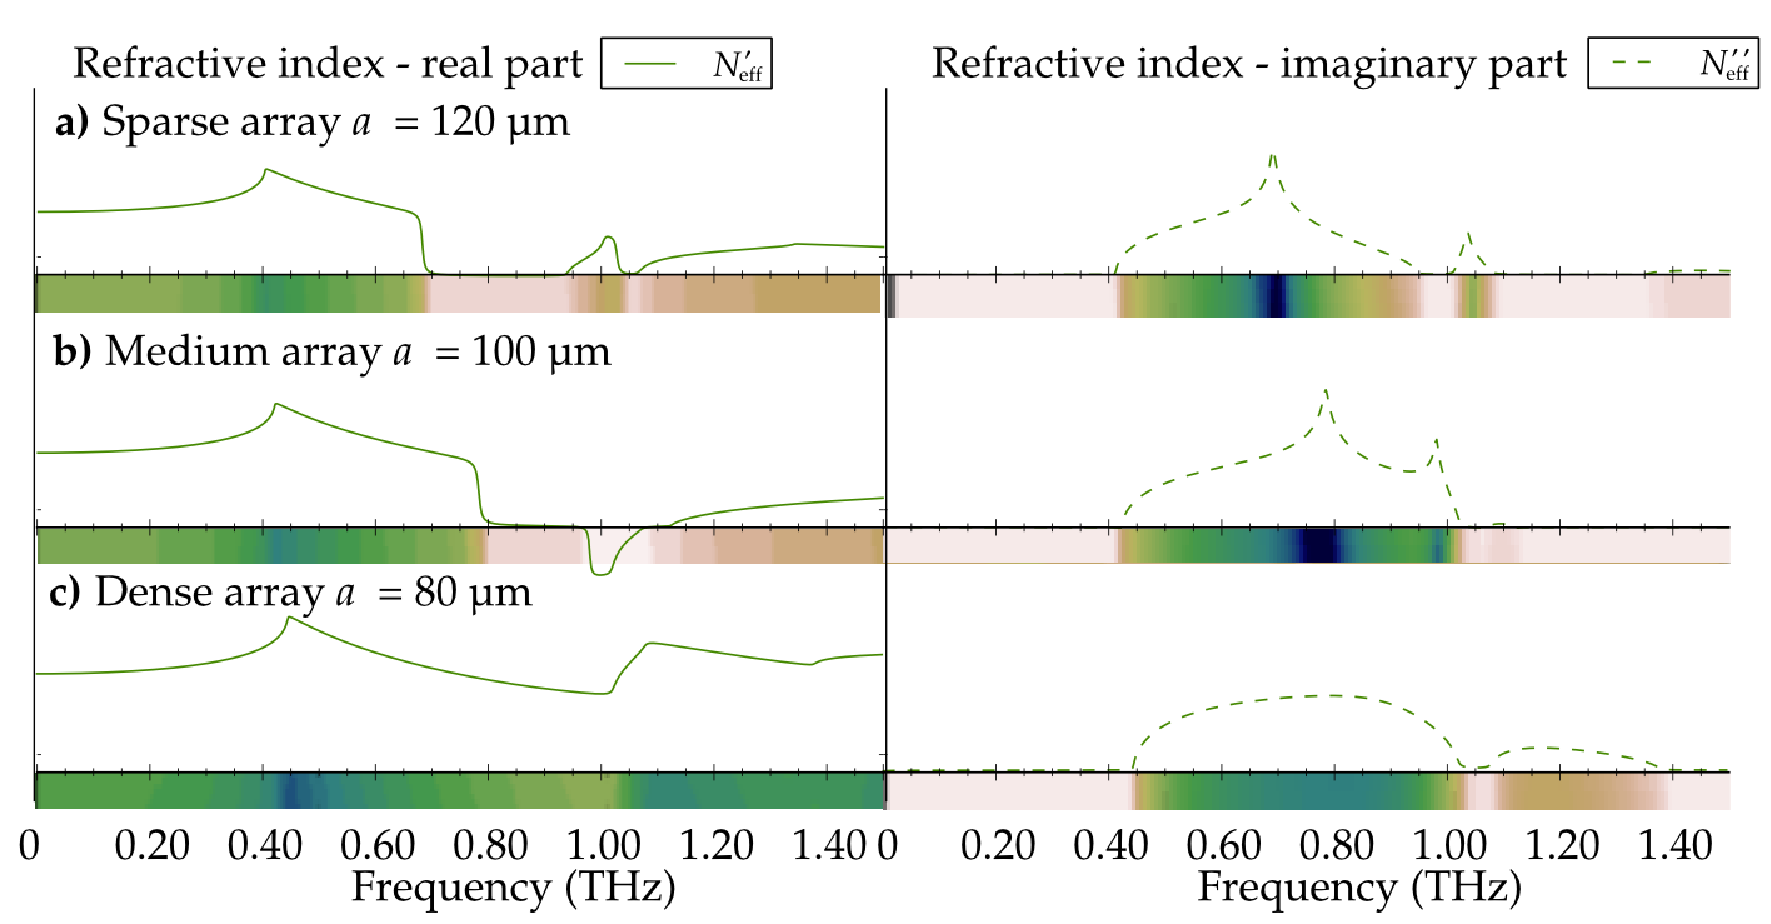
\includegraphics[width=0.5\textwidth]{img/ERods_sketch_of_separate_spectra_to_continuous_scan.pdf}
\caption{} \label{fg_spacingscan100formation}. 
\end{figure}



\begin{figure}\centering  %% TODO rename Re<--->Im
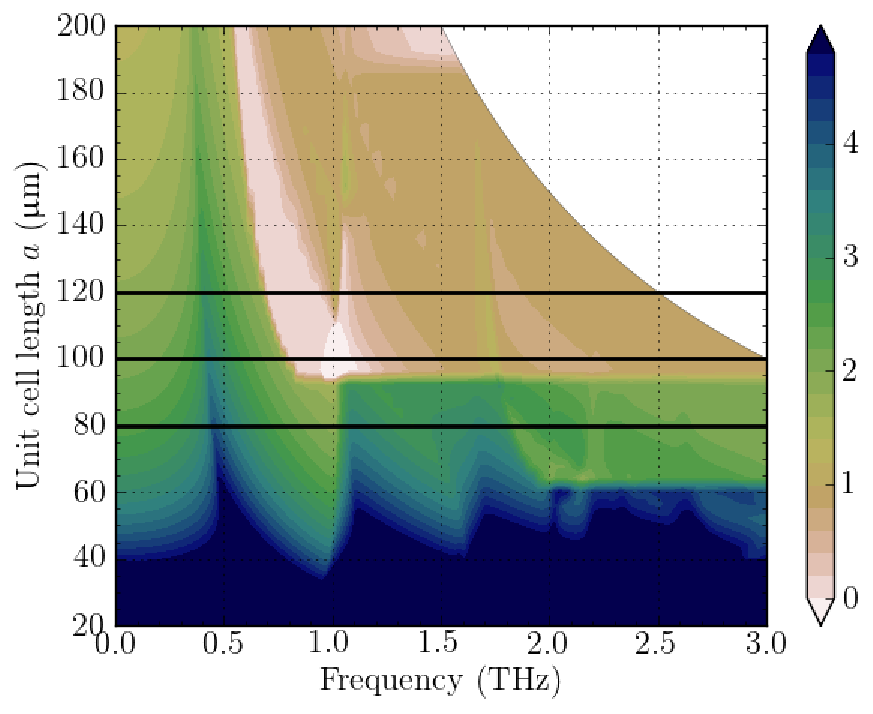
\includegraphics[width=0.5\textwidth]{img/ERods_eps100_spacingscan_Nim.pdf}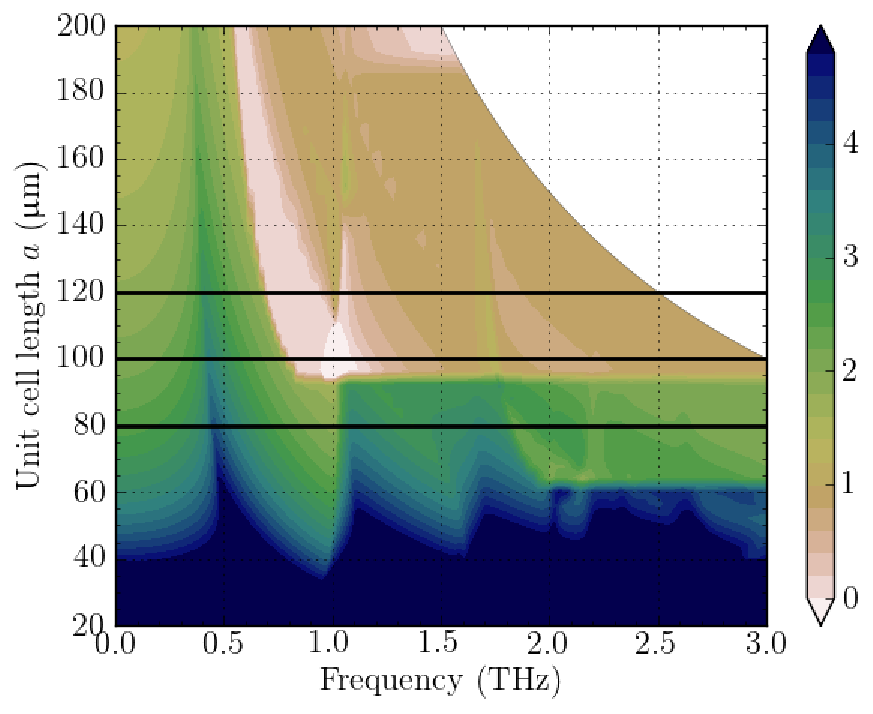
\includegraphics[width=0.5\textwidth]{img/ERods_eps100_spacingscan_Nre.pdf}
\caption{Real ($\Neff'$, left panel) and imaginary ($\Neff''$, right panel) parts of the refractive index for a dielectric rod array with permittivity $\varepsilon_r =100$, radius $\rho = 10$ $\upmu$m and a variable unit cell size $20\:\upmu$m $<a<200\:\upmu$m.  The three solid horizontal lines correspond to the values used in Fig.~\ref{fg_spec}.}
\label{fg_spacingscan100}. 
\end{figure}
%}}}

\paragraph{Continuous scan of the unit-cell size}%{{{
The behavior described above is confirmed by the plots of the complex index of refraction $\Neff',\: \Neff''$ for a continuously varying unit cell size $a$ from 20 to 200~$\upmu$m (Fig.~\ref{fg_spacingscan100}). Here, again, the constant values of the dielectric permittivity $\varepsilon_r=100$ and the rod radius $\rho=10$ $\upmu$m are used. In the upper-right corner of both plots, for $a>c/f$, an empty area is left where the diffraction prevents the determination of effective parameters. 

For an easier interpretation of the results, we draw the most prominent features schematically in Fig.~\ref{fg_drawn100}. Some of them are common in ordinary one-dimensional photonic crystals, namely, the photonic (Bragg) band gaps which are painted in color in Fig.~\ref{fg_drawn100}.

\begin{figure}
    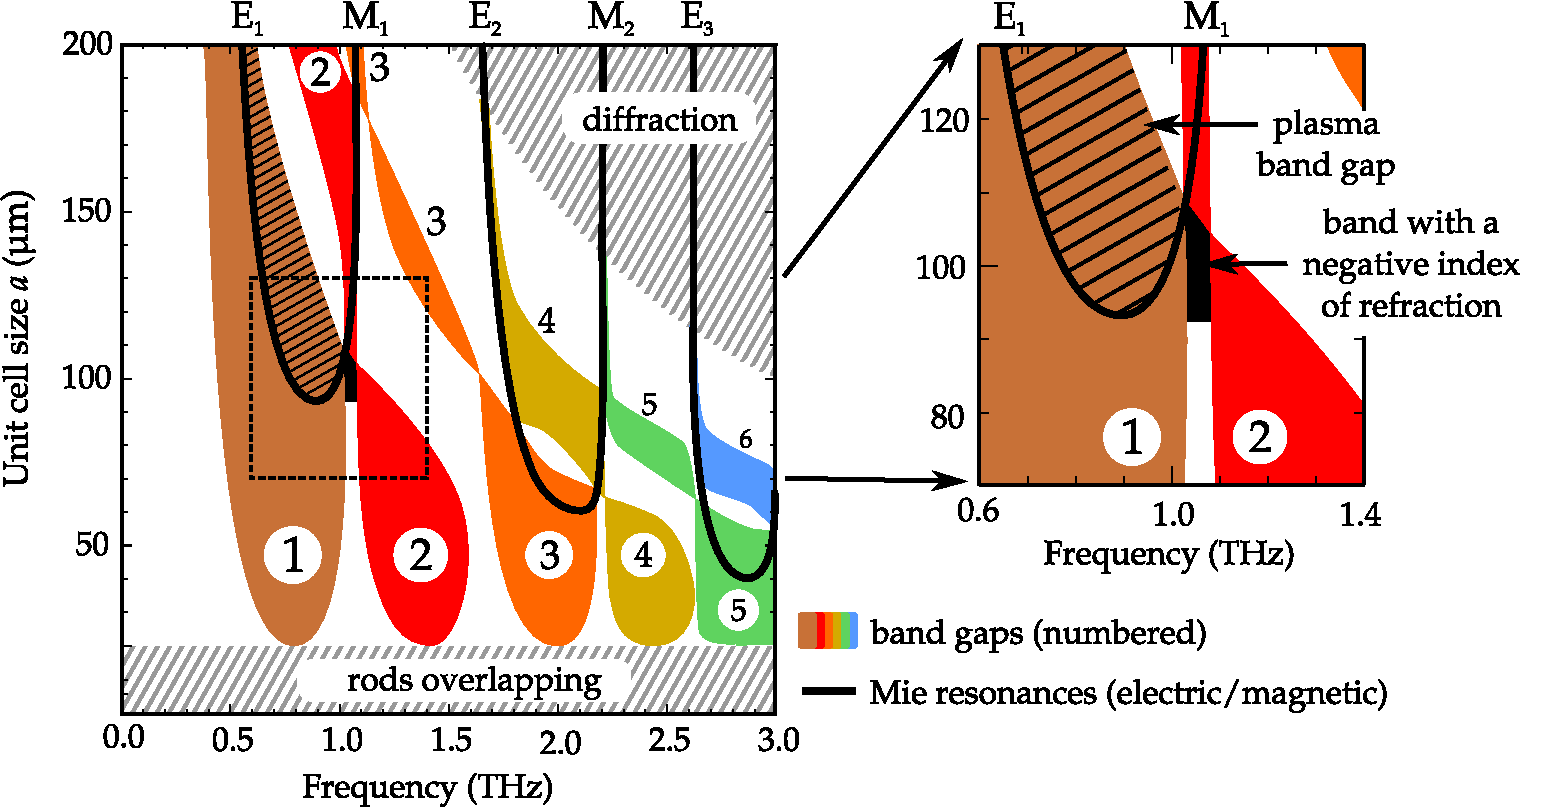
\includegraphics[width=15cm]{img/ERods_eps100_spacingscan_drawn_bands.pdf}
    \caption{Scheme of band gaps and Mie resonances under the same conditions as
    in Fig.~\ref{fg_spacingscan100}.}
\label{fg_drawn100}
\end{figure}




The Mie resonances are caused by the field confinement near the high permittivity elements. They always manifest themselves as sharp peaks in the imaginary part of the index of refraction ($\Neff''$), and in Fig.~\ref{fg_drawn100} they are denoted by thick solid curves. Their electric- or magnetic-dipole character is identified by the letters "E" or "M" above the plot, respectively.

As it can be seen in Figs.~\ref{fg_spacingscan100} and \ref{fg_drawn100}, the pairs of electric and magnetic Mie resonances form U-shaped curves, at the bottom of which the resonances come closer in frequency to each other and eventually they disappear when the unit-cell size $a$ is further reduced. The resonances influence the whole spectra of the refractive index $\Neff'$, so the position of this U-curve delimits the range of $a$ for which a photonic band with $\Neff' < 0$ and $\Neff'' \approx 0$ can be found. This negative-index band is shown in black in Fig.~\ref{fg_drawn100}.

\begin{figure}
	\centering
    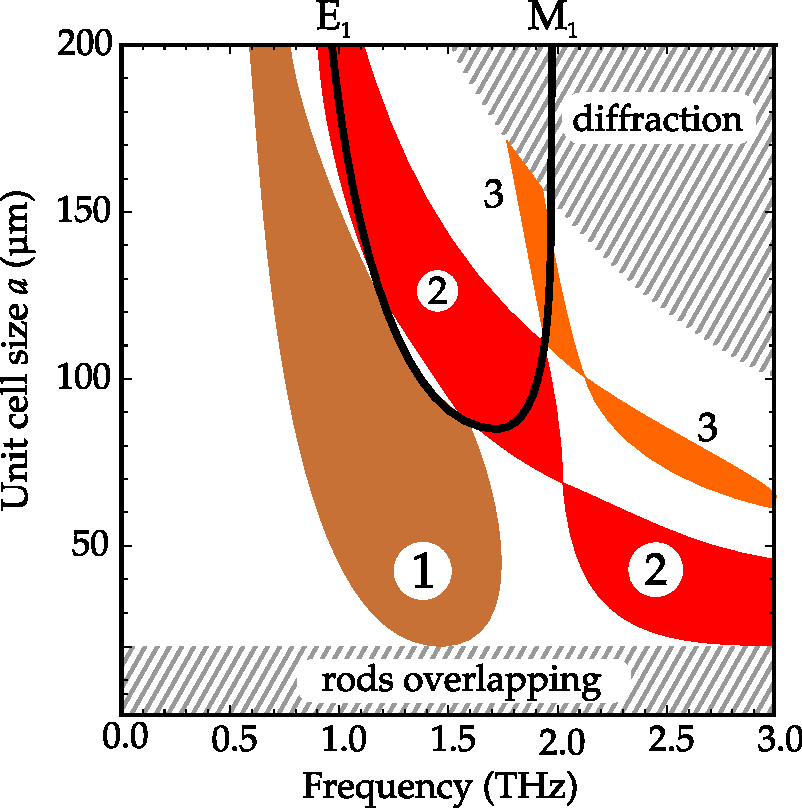
\includegraphics[width=7cm]{img/ERods_eps030_spacingscan_drawn_bands.pdf}
    \caption{Scheme of band gaps and Mie resonances for dielectric permittivity $\varepsilon_r = 30$. The Mie resonances shift to higher frequencies relative to the band gaps and no $\Neff'<0$ region is formed for any unit cell size (cf. Fig. \ref{fg_drawn100})}
\label{fg_drawn030}
\end{figure}

Note that the frequencies of the Mie resonances deviate from their free-space values when the rod distance is reduced. In fact, these resonances help to form the photonic band gaps (both Bragg and plasma band gaps) due to their dispersion. As a consequence, these resonances must be always located inside a frequency range with $\Neff''>0$.
%}}}
\paragraph{Discussion}%{{{
Having analyzed the case of high dielectric ($\varepsilon_r=100$) permittivity rods, we will draw below implications for building a negative-index MM from available dielectrics.  Another series of simulations implies that reducing the dielectric permittivity has the main effect to shift all the Mie resonances to higher frequencies (also with respect to the photonic bands). As a result, the band with $\Neff'<0$ gets gradually narrower and, for the rod permittivity below about 50, we do not find any cell size $a$ that would imply the first and second Mie resonances in the first photonic band as illustrated for $\varepsilon_r = 30$ in Fig. \ref{fg_drawn030}. This means that the value of $\varepsilon_{r} \approx 50$ is the minimum for obtaining a negative index of refraction in any square array of cylindrical rods. Note that one would come to a very similar value of minimum permittivity for the case of a square array of bars with a slightly different shape, e.g. a square cross-section. 

A sufficiently high permittivity can be found in the microwave and terahertz ranges, in a variety of materials, for example in titanium dioxide with $\varepsilon_r \approx 92$ \cite{nemec2009tunable} or in various ferroelectrics like strontium titanate \cite{skoromets2011tuning}. However, practical applications of the high-permittivity dielectrics in the THz range can be restricted by high dielectric losses due to low-frequency phonon absorption tails. To our knowledge, there is no material providing such a high permittivity in the near-infrared or optical ranges. This eliminates the possibility to build a MM at these frequencies with $\Neff'<0$ based on dielectric rods.

Finding a valid negative index of refraction $\Neff'$ for a photonic structure implies that the Snell law can be used to predict the negative refraction at an interface, provided the iso-frequency contours can be well approximated by a circle. This condition is fulfilled when the resulting wave vector is oriented close to a symmetry axis of the structure, or when the wave vector is negligible compared to the reciprocal lattice vector (i.e. $k\ll \frac{\pi}{a}$ and thus $|\Neff'| \ll \frac{c}{2af}$).  In the latter case the iso-frequency contours of the isotropic structure approach a circular shape near the $\Gamma$-point in the Brillouin zone center.  By contrast, the opposite implication is not necessarily applicable---a structure with a high enough spatial dispersion can still refract under negative angles, yet its refractive index computed along a symmetry axis never reaches negative values and the phase difference across each its unit cell is positive and can be comparable to $\pi$.  For example, it was suggested earlier  \cite{vynck2009} that an array of silicon rods ($\varepsilon_r \approx 12$) can constitute a true left-handed metamaterial ($\Neff'<0$).  In agreement with the results presented above, we believe that the negative refraction is not a sufficient proof of $\Neff'<0$, which would require a much higher permittivity contrast than that of silicon.  We conclude that the electromagnetic behavior observed previously \cite{vynck2009} has to be described by means of the PhC dispersion curves. 

We demonstrated that for $\Neff'<0$, not only the high permittivity contrast, but also a correct geometry is required. A wedge filled with an array of square-shaped high-dielectric bars was previously reported refracting under negative angles \cite{peng2007}. The high filling fraction ($0.44^{2}$) simultaneously with a permittivity of $\varepsilon_r \approx 600$ clearly qualified this structure as \textit{dense}. Using the above described approach, we computed its spectra qualitatively similar to Fig.~\ref{fg_spec}(c) and no band with $\Neff' < 0$ was resulting from our effective index retrieval. However, when we reproduced the wedge experiment numerically, our simulations confirmed that it does refract the light under negative angles.

This structure lies at the boundary between the criteria for MMs and PhCs described in the Introduction.  To determine its refraction angle, in general, it is not possible to use the concept of the effective refractive index and its iso-frequency contours have to be used instead (like in PhCs). At the same time, this structure was proved to partially retain negative refraction even under randomization of the positions of the dielectric bars \cite{peng2007}, implying that most of the resonant energy is concentrated inside the dielectric (which is characteristic of MMs).
%}}}



\begin{figure} \caption{img/ERods\_eps100\_R11\_PWEM.pdf}  \centering 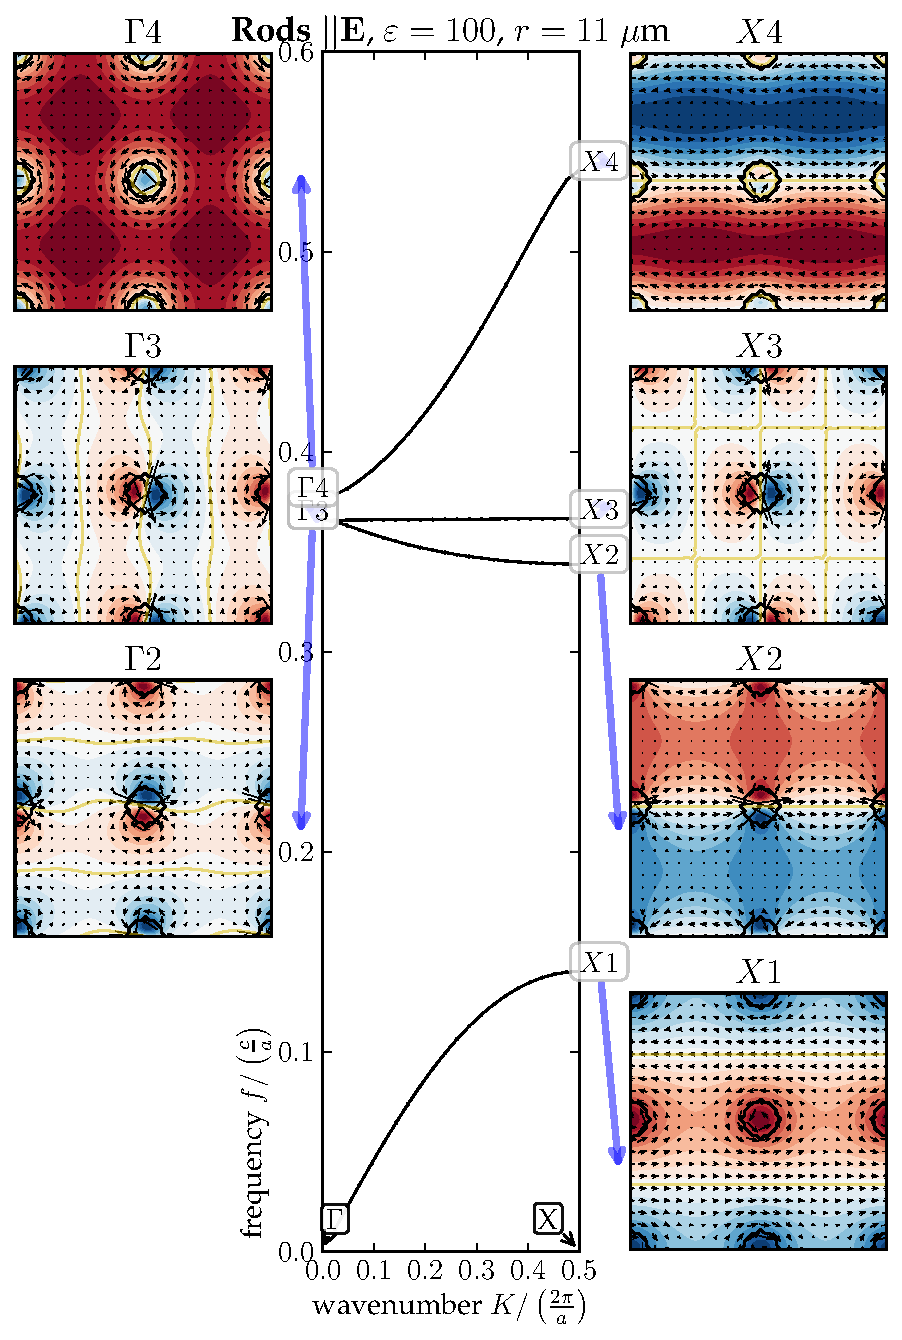
\includegraphics[width=10cm]{img/ERods_eps100_R11_PWEM.pdf} \end{figure} \clearpage
%  \begin{figure} \caption{img/ERods\_eps100\_single\_a120\_FDTD.pdf}  \centering 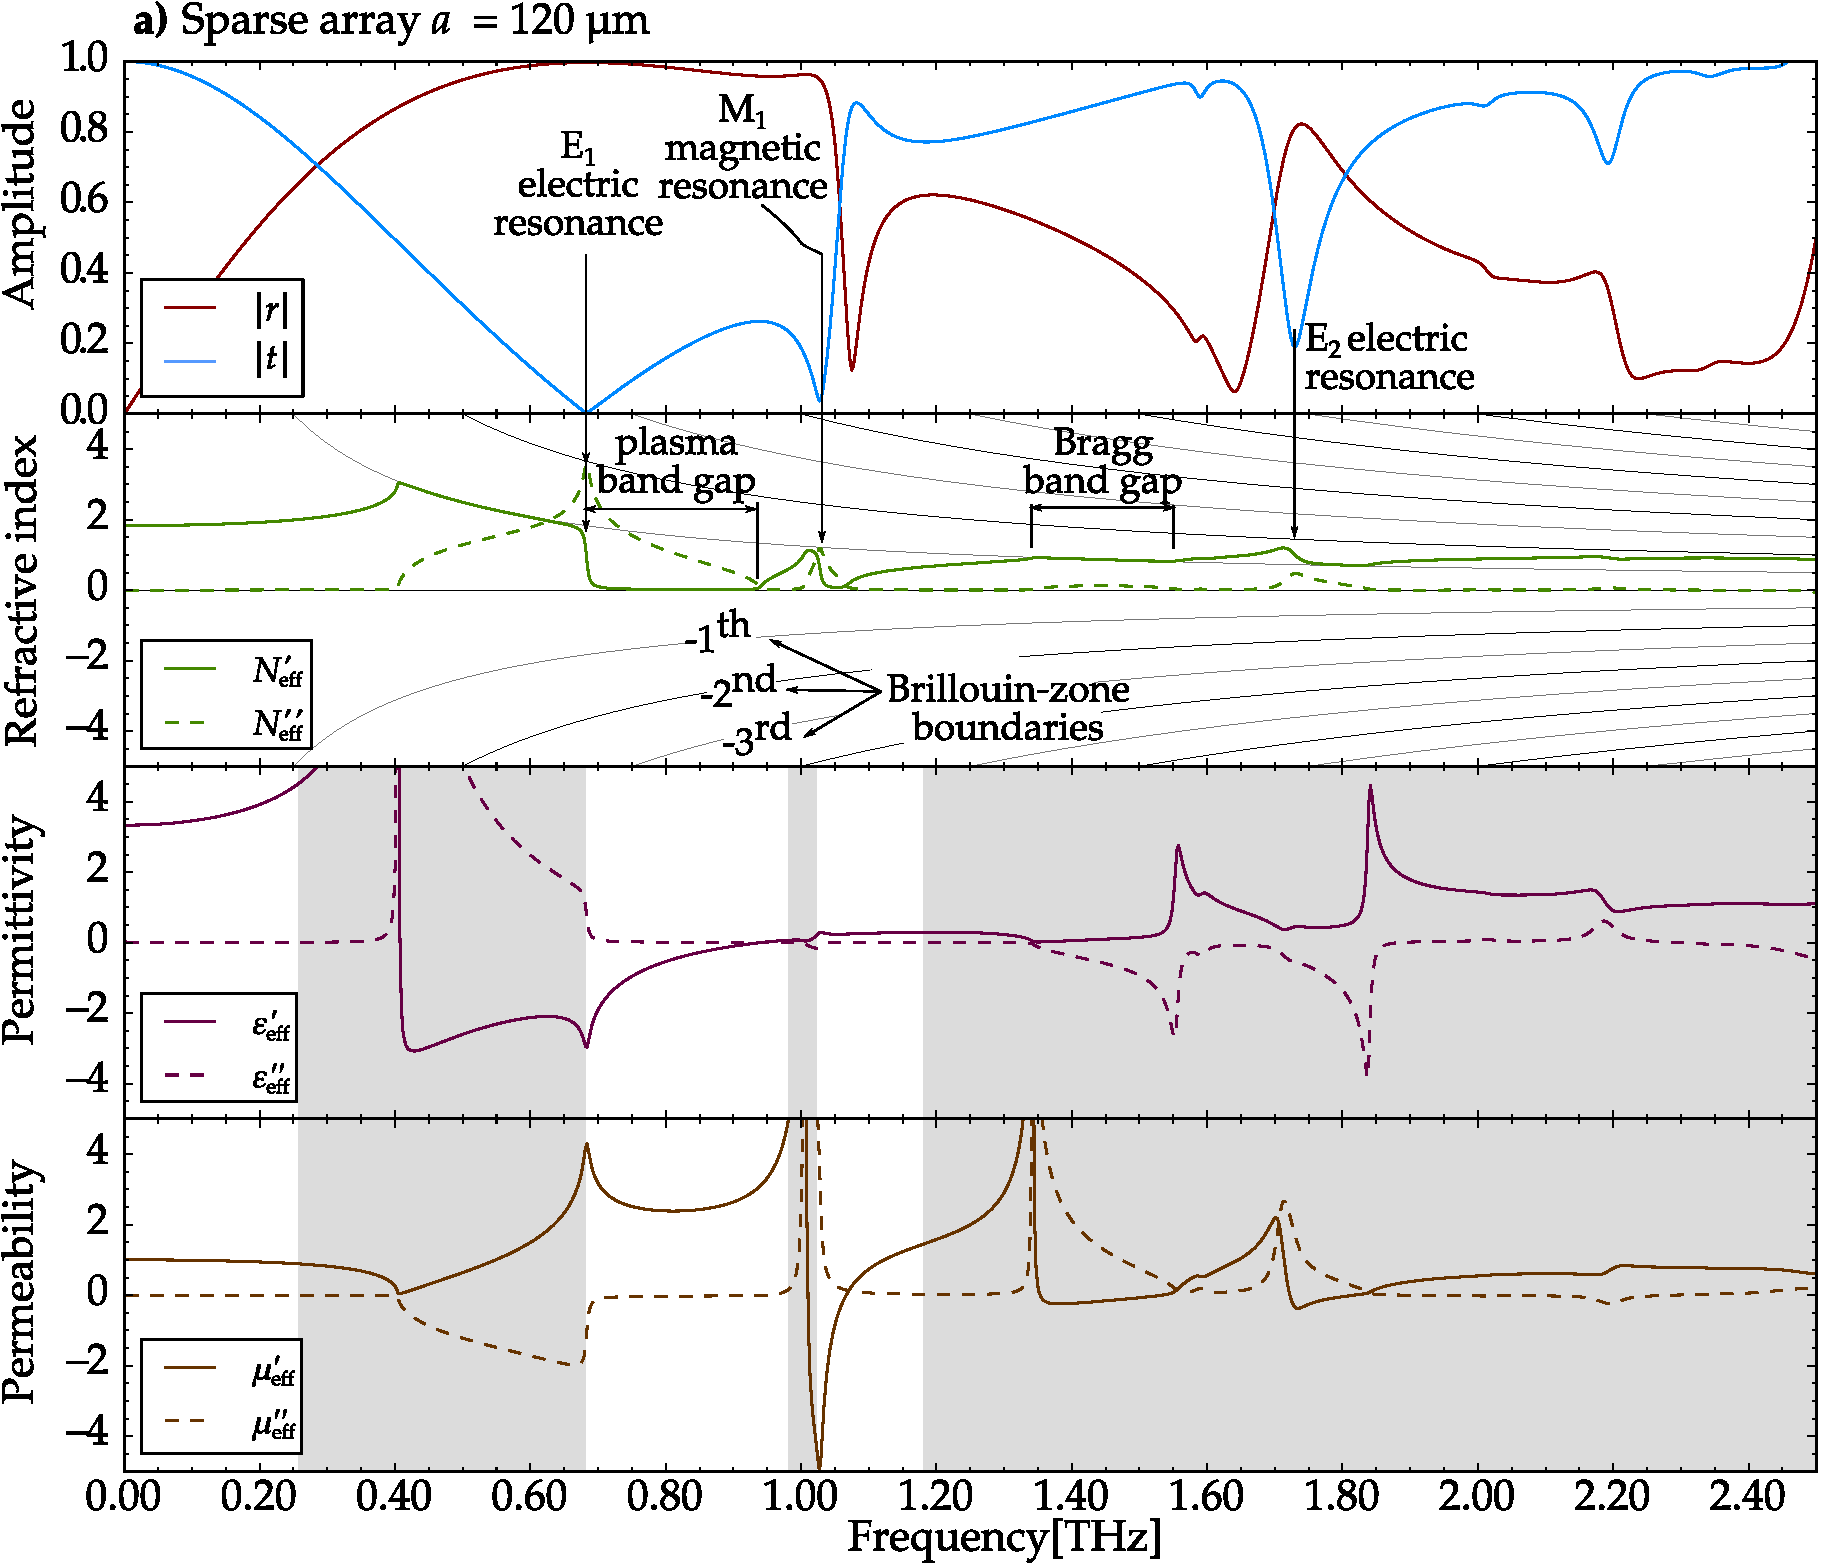
\includegraphics[width=10cm]{img/ERods_eps100_single_a120_FDTD.pdf} \end{figure} \clearpage
%  \begin{figure} \caption{img/ERods\_eps100\_triple\_a150a100a080\_FDTD.pdf}  \centering 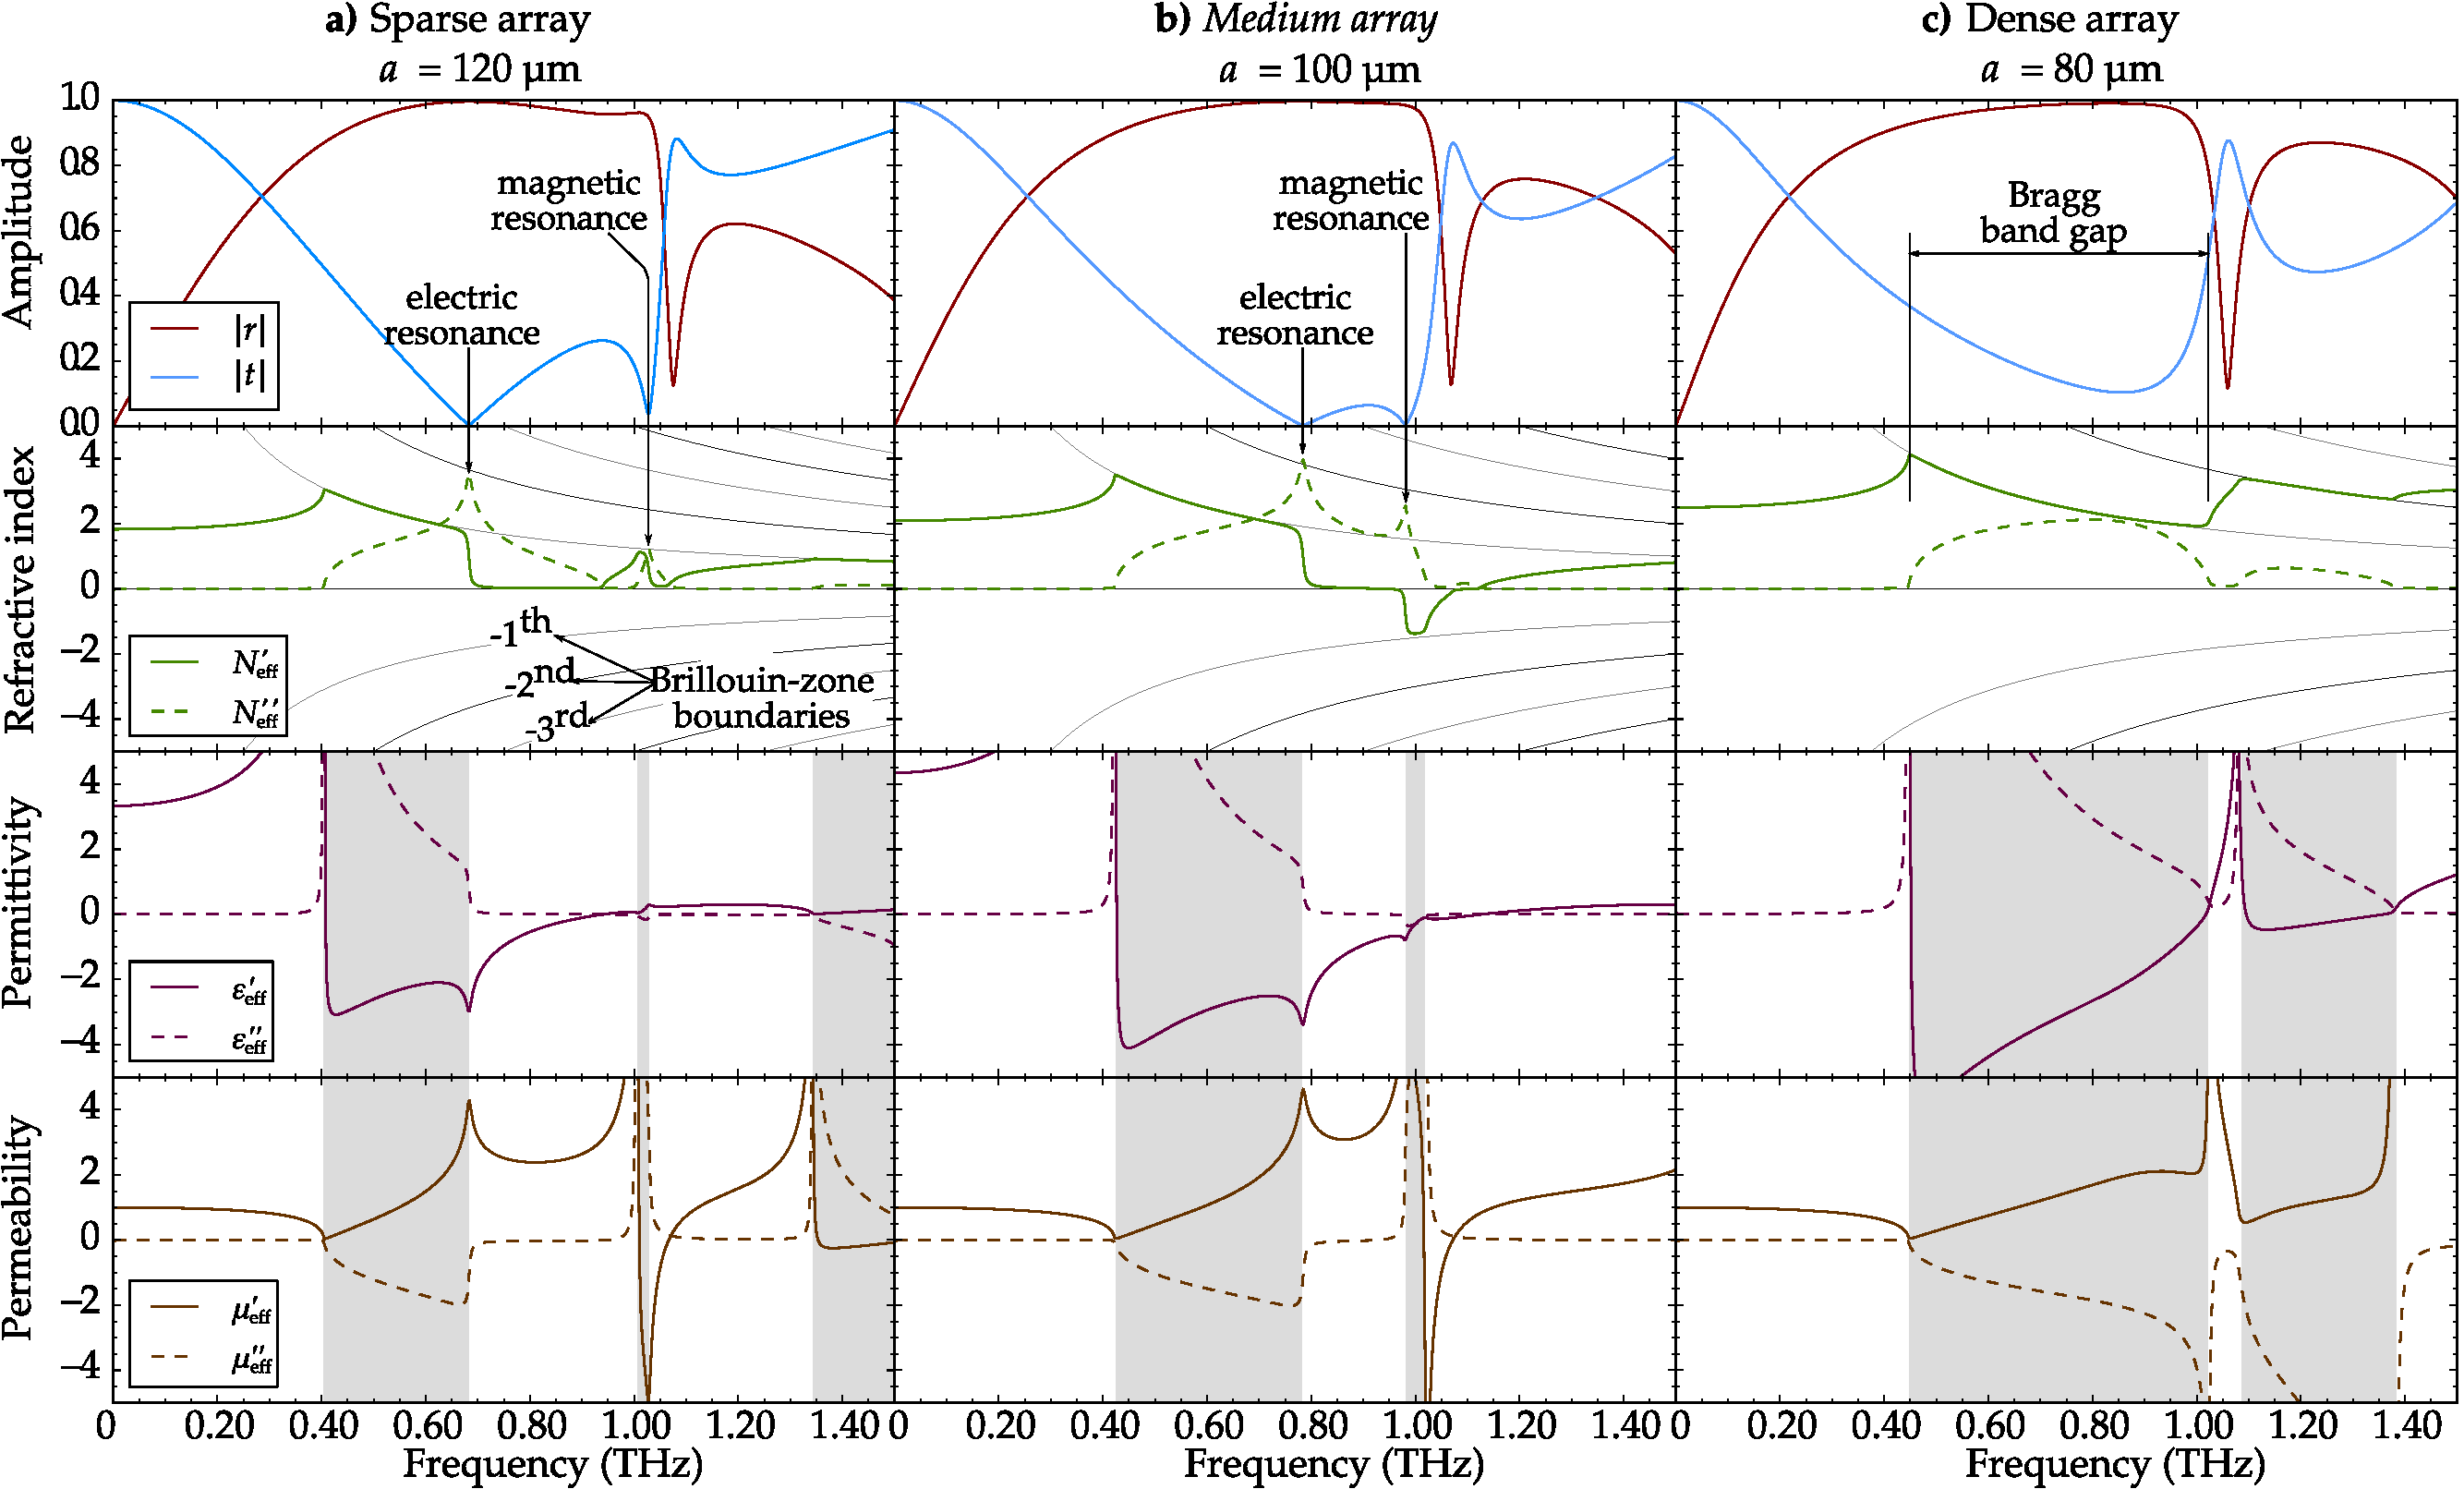
\includegraphics[width=10cm]{img/ERods_eps100_triple_a150a100a080_FDTD.pdf} \end{figure} \clearpage
%  \begin{figure} \caption{img/ERods\_forSeefeld\_sparserN\_denserN\_DrawnBands.pdf}  \centering 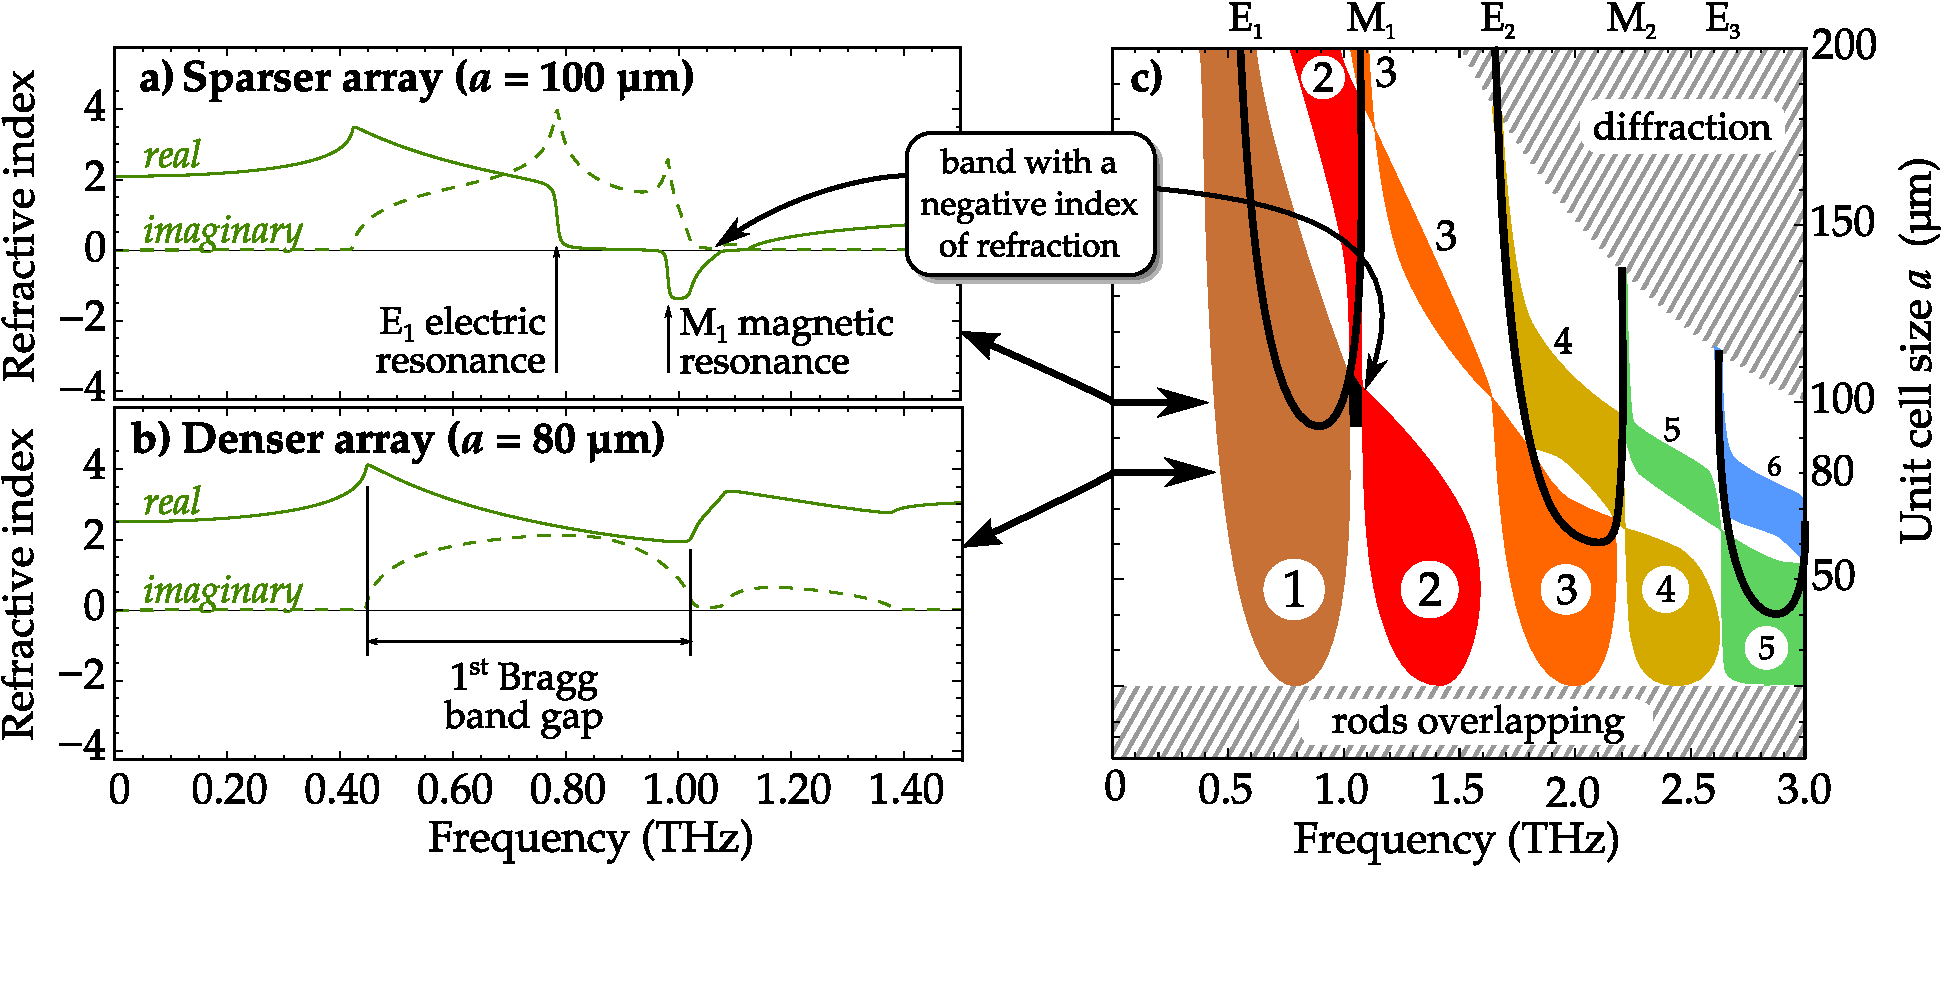
\includegraphics[width=10cm]{img/ERods_forSeefeld_sparserN_denserN_DrawnBands.pdf} \end{figure} \clearpage

\begin{figure} \caption{img/ERods\_sketch\_recordedline.pdf}  \centering  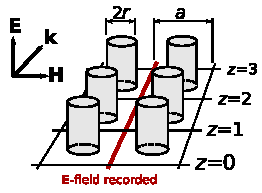
\includegraphics[width=10cm]{img/ERods_sketch_recordedline.pdf} \end{figure} \clearpage
\begin{figure} \caption{img/ERods\_eps100\_R10u5\_FXplot.pdf}  \centering 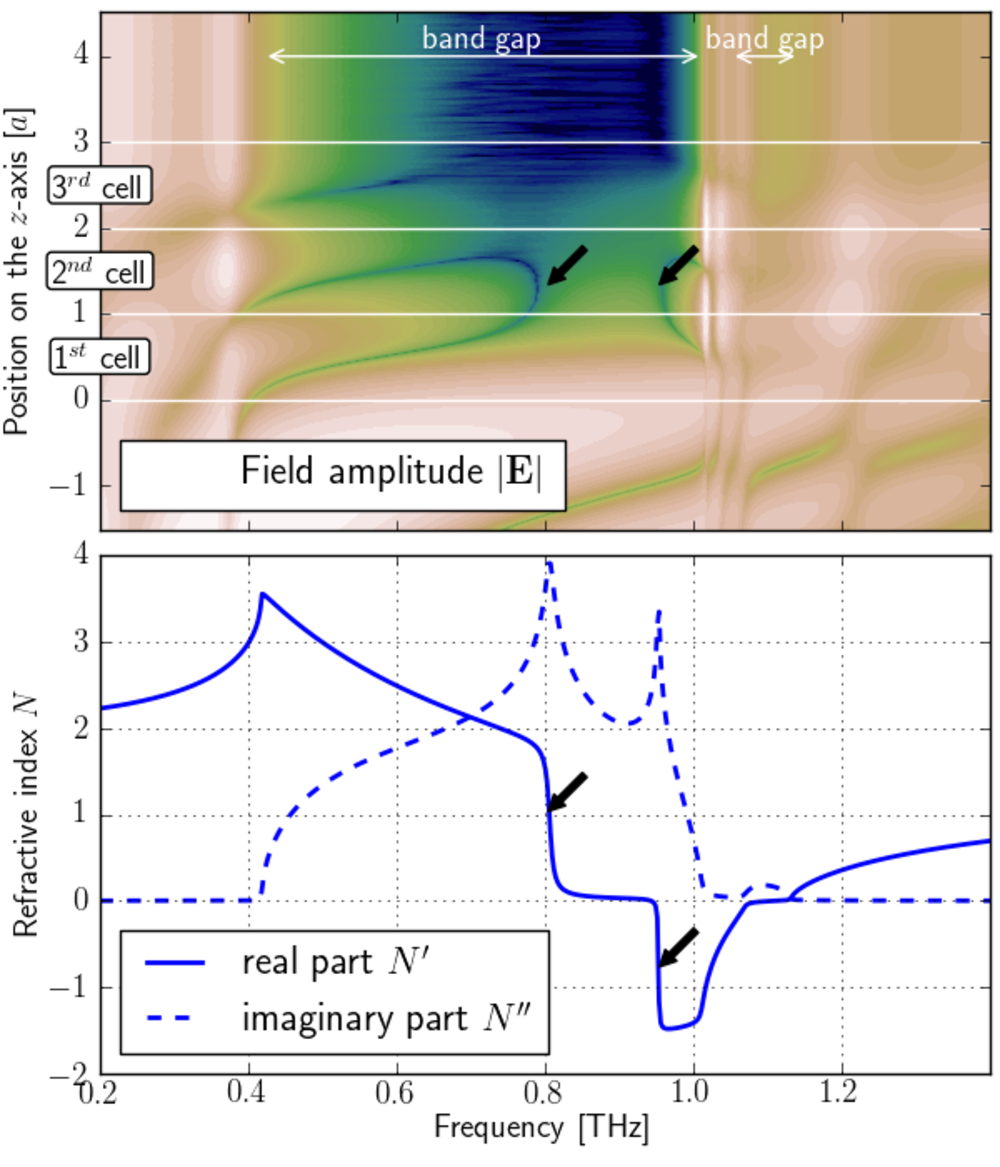
\includegraphics[width=10cm]{img/ERods_eps100_R10u5_FXplot.pdf} \end{figure} \clearpage







%====================================================================================================
\section{Metallic sheet with slits} \label{section_eot} % references to ->
Wood anomaly in hole arrays
Standing SPP wave






%====================================================================================================
\section{Fishnet -- metallic sheet with holes} \label{section_fishnet} % references to ->
%Aperture-array transmission
%Wood anomaly in slit arrays

%Babinet principle
% for nearly flat structures, where most of the fields are confined within a slab perpendicular to $\KK$, a

%surface plasmons, standing/propagating

Perforated plates \cite[p. 58]{brown1953artificial} % http://photonics.inescporto.pt/links/fct2013-1/metap14.pdf
%{{{
\cite{yahiaoui2012metallo,rockstuhl2008light}

The resonance in the metallic mesh has been used as a filter 
\cite{ulrich1967effective,ulrich1967far}
... has been known for half a century \cite{vogel1964transmission}

Improved cross-shaped pattern for better spectral selectivity \cite{porterfield1994resonant}

%}}}







%====================================================================================================
\section{Other structures} % plasmonic spheres (note: resonance width determined by gamma of the metal?)
\cite{croenne2009controle}


\label{endtext} 

\chapter{Appendices}

\section{Appendix A: from Fresnel reflection to $s$-parameter inversion} \label{app_fresnel} % TODO
%\subsection{Frequency-band source for oblique incidence in FDTD} % TODO add this?
\subsection{Fresnel equations} % TODO
\mdf{
also known as Fresnel-Airy function; 
the resulting Fabry-Pérot resonances result in the typical Fresnel-Airy function in the transmittance spectrum;
(note that the term of \textit{Airy function} is used also for completely different functions thorough physics, such as the eigenstate of a particle in sawtooth potential well, or the diffraction pattern from a straigth edge)
}
\subsection{Transmission of a slab} % TODO
\subsection{Derivation of inverse }\label{app_fresnel_inv} % TODO
%% TODO rewrite my "cai-shalaev" notes here


\section{Appendix C: Scripts used for numerical simulations} 
% TODO
% Permittivity spectra of selected materials can be found on % TODO

\section{Appendix D: Notation} % TODO
% Preliminary


%% we will try to build the theory from first principles


\paragraph{Abbreviations used, ordered alphabetically} %{{{
\begin{table}[ht]   \caption{Table of abbreviations}  \label{tb_shortcuts} \centering 
\begin{tabular}{ll}
 \toprule
Abbreviation & Meaning	\\
 \hline
EDB		& (Formulation of Maxwell equations using the $\E$, $\D$ and $\B$ vectors)\\
FDTD 		& Finite-difference time-domain (algorithm)\\
FDFD 		& Finite-difference frequency-domain (algorithm)\\
FEM 		& Finite-element method (algorithm)\\
FFT 		& Fast Fourier transform (algorithm)\\
FRoI 		& Frequency range of interest\\
FDM 		& Filter diagonalisation method (algorithm)\\
GVD 		& Group velocity dispersion \\
IFC		& Isofrequency contours\\
LHM		& Left-Handed Material\\ %% TODO used anywhere?
MM		& Metamaterial\\
NRW 		& Nicolson-Ross-Weir (method for effective parameter retrieval)\\
NGV 		& Negative group velocity\\
PBG		& Photonic band-gap\\
PhC 		& Photonic crystal\\
PML 		& Perfectly matched layers (absorber in simulation)\\
PWEM 		& Plane-wave expansion method (algorithm)\\
RHM 		& Right-Handed Material\\ %% TODO used anywhere?
STO		& Strontium titanate, SrTiO$_3$ (ferroelectric material)\\
SRR		& Split-ring resonator\\
TDTS 		& Time-domain terahertz spectroscopy\\
%TMM			& Transfer-matrix method  (numerical computation)\\
 \bottomrule
 \end{tabular} \end{table}
%}}}

\begin{table}[ht]   \caption{Symbols used, approximately in the order they are introduced in text}  \label{tb_symbols} \centering %{{{
\begin{tabular}{ll}
 \toprule
Symbol & Meaning	\\
 \hline
$\E$ 		& Electric field\\
$\E_0$ 		& Amplitude of the electric field\\
$\D$ 		& Electric displacement\\
$\HH$ 		& Magnetic field\\
$\B$ 		& Magnetic displacement									\vspace{3mm}\\
 
$\varepsilon_0$ &Vacuum permittivity, $8.85\cdot10^{-12}$ F/m\\
$\mu_0$		&Vacuum permeability, $1.25\cdot10^{-6}$ H/m			\vspace{3mm}\\
 
$\ii$		& Imaginary unit, $\ii^2 = -1$\\
$e$ 		& Euler constant, $e = 2.718\ldots$\\
$\pi$ 		& $\pi = 3.141\ldots$\\
$f$			& Frequency\\
$\omega$ 	& Angular frequency, $\omega = 2\pi f$\\
$\kk$ 		& Wave vector in homogeneous media\\
$\KK$ 		& Wave vector of the Bloch wave in periodic media\\
$t$, $\tau$ 		& Time\\
$c$ 		& Speed of light in vacuum, $c=2.998\cdot 10^8$ m/s \\
$f(t), F(\omega)$ & General function in time domain, and its counterpart in Frequency domain \\
$\chi_e(t),\chi_m(t)$	& Electric and magnetic susceptibility in the local approximantion \\ %% TODO separate freq-domain and time-domain susc?
$\chi_e(\omega)$, $\chi_m(\omega)$ 	& Electric and magnetic susceptibility\\
$\epsrl(\omega), \murl(\omega)$ &Relative permittivity and permeability in the local approximation\\
$\epsrn(\omega, \kk)$ &Relative permittivity for nonlocal media\\
$\murn(\omega, \kk)$ &Relative permeability for nonlocal media\\
$\epsLL(\omega, \kk)$ &Relative permittivity in the Landau-Lifshitz ($\E\D\B$) formulation\\
$\Neff$ 	& Effective index of refraction (of periodic media)\\
$\Zeff$ 	& Effective impedance\\
$\eeff, \meff$ 	& Effective permittivity and permeability (of periodic media)\\
$\rr$, $\brho$ 		& Position in space (radius vector)\\
$\mathbf{a}_{1,2,3}$, $a$ 		& Lattice vectors, unit cell size in the cubic lattice \\
$\mathbb{R}$		& Real numbers\\
$\mathbb{Z}$		& Integers\\
$\mathbb{C}$		& Complex numbers\\
$h$ 		& Planck constant, $h = 6.626\cdot 10^{-34}$ J s\\

 \bottomrule
 \end{tabular} \end{table}

\mdf{General notation of vectors and scalars} 
%}}}


\printbibliography
\end{document}
